\cotefile{81}
\scanpage{2}
\unsure{0|O}\quad Cartes sphériques en général
% archive sheet number: 1

\scanpage{3}
Carte sphérique \inserted{(orientée)} avec repère (dans cat. \unsure{isotopiques|isotopique})

\[
\rotatebox{90}{$\simeq$}
\]
\unsure{morphisme|morphismes} $\mathbb P^{1}_{\mathbb C}\overset{f}{\unsure{-|\longrightarrow}}\mathbb P^{1}_{\mathrm C}$ ``spécial'' i.e
\[
 f(0)=0,\quad f(1)=1,\quad f(\infty)=\infty.\quad f\ \text{étale au dessus de }\mathbb P^{1}-\{0,1,\infty\}
\]
\[
\rotatebox{90}{$\simeq$}
\]
fonction rationnelle $f(z)$ telle que $f(0)=\deleted{\unsure{1}}0$, $f(1)=1$, $f(\infty)=\infty$ et telle que pour $z\in\mathbb C$ \deleted{telle que}\inserted{avec} $f(z)\deleted{\in}\notin\{0,\infty\}$ $f'(z)=0$, on ait $f(z)\deleted{\in}=1$ \deleted{\unsure{$\{0,1,\infty$}}$\}$ \inserted{et de plus} $f''(z)\ne0$ (i.e. la ramification de $f$ en $z$ est $2$)\ldots.

\[
\rotatebox{90}{$\simeq$}
\]
couple $P,Q$ \inserted{$[f=P/Q\quad !\,]$} de polynômes $\in\mathbb C(z)$ premiers entre eux \inserted{(i.e. sans zéros communs)} tels que $P(0)=0$, (donc $Q(0)\ne0$) $P(1)=Q(1)$ (donc $\ne0$), $\deg Q<\deg P$ (ces conditions expriment resp\textsuperscript{t} $f(0)=0$, $f(1)=1$, $f(\infty)=\infty$)
% slanted
\margin{On pourrait aussi normaliser \unsure{au lieu de cel|au lieu de cela} par $Q(0)=1$, ou $P$ unitaire, ou $Q$ unitaire\ldots}
normalisés (par exemple) par $P(1)=Q(1)=1$, et tels que pour $z\in\mathbb C$ avec $[f(z)\deleted{\in}\notin\{0,\infty\}, f'(z)=0,\ \mathrm{i.e.}\,]$ \inserted{$P(z)\ne0$,} $Q(z)\ne0$,
\[
 \frac{P'(z)\deleted{Q(z)}}{P(z)}-\frac{Q'(z)}{Q(z)}=0,
\]
on ait $P(z)=Q(z)$, et de plus
\[
 \frac{P''(z)}{P(z)}-\frac{Q''(z)}{Q(z)}\ne0\qquad\text{i.e.}\quad P''(z)\ne Q''(z)\ldots
\]
[ NB on a
\[
\begin{aligned}
 Q(z)P'(z)-P(z)Q'(z)&=\deleted{Q(z)[P'(z)-P(z)]+P(z)(Q(z)-Q'(z))}\\
 &\phantom{=}\inserted{(Q(z)-P(z))P'(z)+P(z)(P'(z)-Q'(z))}
\end{aligned}
\]
donc si \inserted{pour $P(z);Q(z)\ne0$} cette quantité est nulle, (i.e. $f'(z)=0$), alors $P(z)=Q(z)$ \deleted{\unsure{au|ou}} i.e $Q(z)-P(z)=0$ implique $P'(z)=Q'(z)$ et inversement si $P'(z)=Q'(z)$ on a $(Q(z)-P(z))P'(z)=0$ donc \uline{si} $P'(z)\ne0$, on a $P(z)=Q(z)$ ! Mais peut-on avoir $P'(z)=0$ (d'où aussi $Q'(z)=0$) \inserted{avec $P'(z)=Q'(z)$}\unsure{$\}$|)} sans avoir $P(z)=Q(z)$ ?

\deleted{\unsure{Réfléchissons} $Q(T)=$}

Prenons p.ex. $Q(T)=1$, les conditions sur $P$ deviennent $P(0)=0$, $P(1)=1$, $\deg P\geq1$ \inserted{(conséquence des deux précédentes)}, donc $P(T)=\unsure{T}P_0(T)$ où on a $P_0(1)=1$, la question devient si on peut avoir \inserted{(pour $P(z)\ne0$)} $P'(z)=0$ sans avoir $P(z)=1$ certes oui p.ex. $\deleted{P(T)=T^2}$ si $P(T)=T(aT+b)=aT^2+bT$, $a+b=1$, on a
% margin note written sideways
\margin{\raggedright $P'(T)=2aT+b$ qui est nul \inserted{(supposons $a\ne0$)} pour $z=-\frac{b}{2a}$ \deleted{\unsure{sera}} $\ne\left\{\begin{smallmatrix}0\\-\frac{b}{a}\end{smallmatrix}\right.$ \deleted{\illegible{1}} les deux zéros de $P$ si $b\ne0$, et $P(-\frac{b}{2a})=-\frac{b}{2a}(-\frac b2+b)=-\frac{b^2}{4a}$ qui \deleted{\unsure{peut être}} est $\ne1$ \deleted{\unsure{en prenant}} si $b^2\ne-4a$---}
% archive sheet number: 2

\scanpage{4}
% Whole-page cancellation: two long diagonal strokes cross the two columns.
% Local cancellations are nested inside the whole-page deletion state.
\[
\deleted{\begin{aligned}
 f_{d-2}e_1&=-e_{d-2}f_1\qquad(=\unsure{\eta|\gamma}_{d-1}\unsure{\}|\,}=\eta)\\
 \delta(\eta)&=e_{d-2}
\end{aligned}}
\]
\[
\deleted{\underline{\boxed{\begin{gathered}
(1\leq i\leq d-2)\\
\left\{\begin{aligned}
e_i e_1&=0\qquad f_i f_1=\begin{cases}0&\text{si }i\text{ impair}\\f_{i+1}&\text{si }i\text{ pair}\end{cases}\\
f_i e_1&=e_{i+1}\\
e_i f_1&=\begin{cases}-e_{i+1}&\text{si }i\text{ impair}\\0&\text{si }i\text{ pair}\end{cases}\qquad\unsure{\text{''}}
\end{aligned}\right.
\end{gathered}}}}
\]
% Two isolated quotation-like ticks stand at the right inside the box.
% A separate lower rule retraces the frame; the underline preserves the second lower stroke.
\[
\deleted{xf_1=f_1x=0\quad\text{si }\deg x\text{ pair}\qquad
 \eta=e_{d-1}\quad\delta(e_{d-1})=e_{d-2}}
\]
\[
\deleted{\unsure{\cdot}\quad\deleted{xf_1}}
\]
\[
\deleted{\begin{aligned}
 &(f_i+\lambda e_{\unsure{i|1}})(f_1+\lambda e_1)\\
 &=\underset{\inserted{f_{i+1}}}{\deleted{f_i f_1}}+\lambda^2\deleted{e_i e_1}
 +\lambda\bigl(\underbrace{f_i e_1}_{\inserted{e_{i+1}}}+
 \underbrace{\deleted{e_i f_1}}_{\inserted{\deleted{\unsure{-|\,}e_{i+1}}}}\bigr)
\end{aligned}}
\]
\[
\deleted{\begin{aligned}e_2&=f_1e_1\\e_3&=f_2e_1\end{aligned}}
\]
% margin note written upside down
\margin{\deleted{$\deleted{e_1 f_d}$}\quad
\deleted{$e_i e_1=0\qquad 1\leq i\leq d-2$}\quad
\deleted{$f_i f_1=$}}
\[
\deleted{\deleted{\delta(e_i e_j)=\unsure{0}}\qquad\delta(e_i e_j)=}
\]
\[
\deleted{\begin{gathered}
1\leq i\leq d-2\\
\left\{\begin{aligned}
e_i e_1&=0\\
f_i f_1&=\begin{cases}0&\text{si }i\text{ impair}\\ f_{i+1}&\text{si }i\text{ pair}\end{cases}\\
f_i e_1&=\eta_{i+1}=\alpha e_{i+1}+\beta f_{i+1}\\
e_i f_1&=\begin{cases}
\overset{\inserted{-}}{\deleted{\unsure{a|0}}}\eta_{i+1}=-\alpha e_{i+1}-\beta f_{i+1}&i\text{ impair}\\
-\eta_{i+1}+e_{i+1}=(1-\alpha)e_{i+1}-\beta f_{i+1}&i\text{ pair}
\end{cases}
\end{aligned}\right.
\end{gathered}}
\]
\[
\deleted{\underline{f_1e_1\deleted{f_1}=-e_1f_1=\eta_2=\alpha e_2+\beta f_2}}
\]
\[
\deleted{\begin{array}{c l}
1\leq i\leq d-3&\\
(e_i f_1)e_1&=\deleted{\unsure{-e_i}}
\begin{cases}
-\eta_{i+1}e_1=-\beta f_{i+1}e_1=-\beta\eta_{i+2}&i\text{ imp}\\
-\eta_{i-1}e_1+\deleted{e_{i+1}e_1}=-\beta\eta_{i+2}&i\text{ pair}
\end{cases}\\
\rotatebox{90}{$=$}&\\
e_i(f_1e_1)&\deleted{=e_i\eta_2=e_i(\alpha e_2+\beta\unsure{\bar f_2|\vec f_2|f_2})}\\
\rotatebox{90}{$=$}&\\
-e_i(e_1 f_1)&\\
\rotatebox{90}{$=$}&\\
-(e_i e_1)f_1=0&\text{donc}\quad
\tikz[baseline=(a.base)]\node[draw,circle,inner sep=1pt] (a) {$\beta=0$};\quad\alpha=\pm1
\end{array}}
\]
\[
\deleted{\text{donc}\quad\delta\eta=\pm e_{d-2}\qquad\unsure{Q\Phi S|QDS|QPS|QFS}}
\]
\[
\deleted{\begin{aligned}
\eta&=f_{d-2}e_1\\
\delta\eta&=\delta(f_{d-2})e_1=f_{d-3}e_1.
\end{aligned}}
\]
% Faint unassigned surface traces at lower right and above e_2 were inspected; no secure character was assigned.
% archive sheet number: 3

\scanpage{5}
\(\overset{\hspace{0.55em}\unsure{?}}{\text{\uline{NB}}}\)\quad Si $\sigma$ est un $\underset{\hspace{-1.3em}\unsure{\cdot}}{\text{automorphisme}}$ du corps des complexes, et si $f$ est ``spécial'', alors $f^\sigma$ est \unsure{égalmt|également} spécial -- donc $\operatorname{Aut}(\mathbb C)$ opere sur l'ens des $f$ spèciaux. Mais il opère par l'intermédiaire de $\operatorname{Aut}(\unsure{\overline{\mathrm Q}|\overline{\mathbb Q}})$, car si $f=P/Q$ spécial, les $\underset{\hspace{1.5em}\unsure{-|=}}{\text{coeff.}}$ de $P,Q$ sont des \uline{nbs algébriques}. Il revient au $=$ de dire que les zéros de $P,Q$ sont des nbs algébriques, i.e. le diviseur de $f$ est

% A pale hook and dark dot above NB are retained as an unsure question-like shape.
% A tiny detached dot below automorphisme is retained; its function is uncertain.
% Faint detached strokes below the right end of coeff. are preserved above;
% the mark's origin and intention remain unresolved (full scan x409--436, y887--902).
% The following drawing preserves the relative placement of four detached
% lower mark-groups. The three uncertain groups have unresolved intention;
% no mathematical relation between them is supplied.
\figure{\begin{tikzpicture}[x=0.011cm,y=0.011cm]
  \node[inner sep=0pt] at (489,161) {$\unsure{\cdot\,\cdot|-}$};
  \node[inner sep=0pt] at (0,0) {$\unsure{-|=}$};
  \node[inner sep=0pt] at (61,5) {$\unsure{\frown|-}$};
  \node[inner sep=0pt] at (545,0) {$-$};
\end{tikzpicture}}
% archive sheet number: 4

\scanpage{6}
\[
\begin{aligned}
(P/Q)'&=\frac{P'}{Q}-P\frac{Q'}{Q^2}=\frac{P'Q-Q'P}{Q^2}\\
(P/Q)''&=P''/Q\deleted{\unsure{+}}\unsure{-|+}2\frac{P'Q'}{Q^2}+\deleted{\unsure{2}}P\bigl(
\end{aligned}
\]
\[
\frac{P'}{\deleted{Q}P}-\frac{Q'}{Q}
\]
\[
(xy)^{\unsure{2|''}}=\unsure{x''|x^2}y+2x'y^{\unsure{\prime}}+xy^{\unsure{\prime\prime|\prime}}
\]
\[
\left(\frac{\deleted{\unsure{P'}}f}{g}\right)'=\frac{f'g-g'f}{g^2}
\]
\[
\frac{(P''Q+\deleted{P'Q'}-\deleted{P'Q'}\deleted{\unsure{+}}\unsure{-|+}Q''P)Q^{\unsure{\deleted{2}|2}}
 -(P'Q-Q'P)2\deleted{Q}Q'}{Q^3}
\]
% The second fraction rule follows the separate lower tracing beneath the right-middle part.
\figure{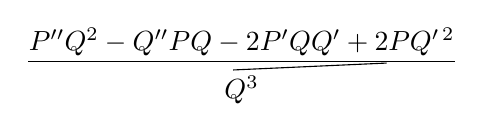
\begin{tikzpicture}
\node[inner sep=0pt,anchor=south west] (num) at (0,0)
 {$P''Q^2-Q''PQ-\unsure{2}P'QQ'+2PQ'^{\,2}$};
\path (num.south west)--(num.south east) coordinate[pos=0.48] (partialstart);
\path (num.south west)--(num.south east) coordinate[pos=0.84] (partialend);
\draw ([yshift=-2pt]num.south west)--([yshift=-2pt]num.south east);
\draw ([yshift=-5pt]partialstart)--([yshift=-2.5pt]partialend);
\node[inner sep=0pt,anchor=north,yshift=-7pt] at (num.south) {$Q^3$};
\end{tikzpicture}}
% The small quotient's fraction rule turns back at its right end; no arrow meaning is assigned.
\figure{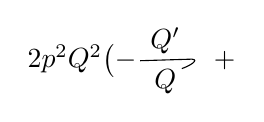
\begin{tikzpicture}
\node[inner sep=0pt,anchor=base west] (prefix) at (0,0) {$2p^2Q^2\bigl(-$};
\node[inner sep=0pt,anchor=south] at ([xshift=0.36cm,yshift=0.08cm]prefix.east) {$Q'$};
\node[inner sep=0pt,anchor=north] at ([xshift=0.36cm,yshift=-0.10cm]prefix.east) {$Q$};
\draw ([xshift=0.04cm]prefix.east)--([xshift=0.70cm,yshift=0.02cm]prefix.east)
 .. controls ([xshift=0.80cm,yshift=0.01cm]prefix.east) and ([xshift=0.66cm,yshift=-0.07cm]prefix.east)
 .. ([xshift=0.57cm,yshift=-0.10cm]prefix.east);
\node[inner sep=0pt,anchor=west] at ([xshift=0.97cm]prefix.east) {$+$};
\end{tikzpicture}}

% Opposite-direction writing, read after a half-turn. Two long diagonals cancel this layer.
\[
\deleted{\det\begin{pmatrix}a\deleted{\unsure{d|b}}&c\\b&d\end{pmatrix}-ad-bc\quad\text{inversible}}
\]
\[
\deleted{\begin{array}{c@{}l}
\delta(e_1 e_{d-2})&=-e_1\delta(e_{d-2})=-e_1e_{d-3}\deleted{=e_d}\\
\rotatebox{90}{$=$}&\\
\delta(a\eta)&=a\delta\eta=a\alpha e_{d-2}+a\beta f_{d-2}
\end{array}}
\]
\[
\deleted{\begin{array}{c@{}l}
\delta(e_1 f_{d-2})&=-\deleted{f}e_1\cdot f_{d-3}\\
\rotatebox{90}{$=$}&\\
b\alpha e_{d-2}+b\beta f_{d-2}&
\end{array}}
\]
\[
\deleted{\begin{array}{c@{}l}
\delta(f_1 e_{d-2})&=\delta(f_1)e_{d-2}-f_1\delta(e_{d-2})=e_{d-2}-f_1e_{d-3}\\
\rotatebox{90}{$=$}&\\
\delta(c\eta)&=c\delta\eta=c\alpha e_{d-2}+c\beta f_{d-2}
\end{array}}
\]
\deleted{etc}

% Detached dot at full-scan x=965--973, y=598--607, below and left of On after rotation.
% Its hand, layer, role, and cancellation state are unresolved; no relation to the formula is assigned.
\(\underset{\unsure{\text{.}}}{\phantom{\text{On}}}\)\deleted{On en tire $e_1e_{d-3}$, $\deleted{f}e_1f_{d-3}$\unsure{,} $f_1e_{d-3}$, $f_1f_{d-3}$ comme comb. lin des $e_{d-1}$ et $f_{d-2}$, à coeff entiers fonctions de $\alpha,\beta$, $a,b,c,d$}

\[
\deleted{\begin{array}{c@{}l}
\delta(e_1x_i)&=-e_1\delta(x_i)=-e_1\deleted{\unsure{\delta}}x_{i-1}\qquad 2\leq i\leq{}\\
\rotatebox{90}{$=$}&\\
\delta(\deleted{\unsure{S}}s e_{i+1}+t f_{i+1})&=s e_i+t f_i
\end{array}}
\]
% archive sheet number: 5

\scanpage{7}
\deleted{\illegible{1}} Soit $a\in\mathbb N^*,b\in\mathbb N^*,c\in\mathbb N^*,\ q\in\mathbb N^*$ \quad $q$ nombre premier $(q\ne1)$

On suppose que $a\mathrel{\underset{1}{\smile}}b$, $a\mathrel{\underset{1}{\smile}}c$, $b\mathrel{\underset{1}{\smile}}c$ (premiers entre eux deux à deux)
\inserted{et $a^q+b^q=c^q$}

On a $c>a$ et $c>b$ car $a\in\mathbb N^*$ et $b\in\mathbb N^*$

On pose $c=a+b'=b+a'$ avec $b'\in\mathbb N^*$ et $a'\in\mathbb N^*$
\[
\begin{aligned}
\text{alors}\qquad a^q+b^q=c^q&=(a+b')^q=\sum_{i=0}^{q}C_q^i\,a^i b'^{\,q-i}\qquad\text{(Newton)}\\
 &=b'^{\,q}+\sum_{i=1}^{q-1}C_q^i\,a^i b'^{\,q-i}+a^q\qquad(\text{car }q\geqslant2)
\end{aligned}
\]
\[
\text{donc}\qquad b^q=\sum_{i=1}^{q-1}C_q^i\,a^i b'^{\,q-i}+b'^{\,q}\tag*{(1)}
\]
la puissance de $b'$ n'étant jamais nulle on peut mettre $b'$ en facteur dans le second membre de (1), donc $b'\mid b^q$ ($b'$ divise $b^q$)

Soit $p$ un nombre premier % The phrase is visibly drawn once by rlap. The phantom preserves its deletion
% annotation and text dimensions without adding the generic horizontal rule.
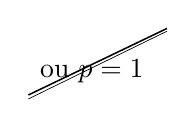
\begin{tikzpicture}[baseline=(cancelled.base)]
\node[inner sep=0pt,outer sep=0pt] (cancelled)
 {\rlap{ou $p=1$}\phantom{\deleted{ou $p=1$}}};
\draw[line width=.55pt] ([xshift=-1.5mm,yshift=-1.5mm]cancelled.south west) -- ([xshift=3mm,yshift=4mm]cancelled.north east);
\draw[line width=.25pt] ([xshift=-1.5mm,yshift=-2mm]cancelled.south west) -- ([xshift=3mm,yshift=3.65mm]cancelled.north east);
\end{tikzpicture}
 et tel que : $p\mid b'$ donc $p\mid b$. Soit $\alpha\in\mathbb N^*$ et $\alpha'\in\mathbb N^*$ tels que
\[
\begin{aligned}
 &p^{\alpha'}\mid b'\quad\text{et}\quad p^{\alpha'+1}\nmid b'\\
 \text{et}\quad &p^\alpha\mid b\quad\text{et}\quad p^{\alpha+1}\nmid b
\end{aligned}
\]
\margin{$\unsure{a|\alpha}$ \unsure{n'exist|n'existe} pas si on avait $p=1$}
On a $\alpha'\leqslant q\alpha$ car $b'\mid b^q$

\[
\begin{aligned}
(1)\ \Longrightarrow\quad&p^{q\alpha}\mid\sum_{i=1}^{q-1}C_q^i\,a^i b'^{\,q-i}+b'^{\,q}\\
\Longrightarrow\quad&p^{q\alpha}\mid b'\left(\sum_{i=1}^{q-1}C_q^i\,a^i b'^{\,q-i-1}+b'^{\,q-1}\right)\qquad(\text{car }q\geqslant2)
\end{aligned}
\]
posons $b'=p^{\alpha'}b''$ donc $b''\mathrel{\underset{1}{\smile}}p$ (propriété de $\alpha'$)
\[
\begin{aligned}
\Longrightarrow\quad&p^{q\alpha}\mid p^{\alpha'}b''\left(\sum_{i=1}^{q-1}C_q^i\,a^i b'^{\,q-i-1}+b'^{\,q-1}\right)\\
\Longrightarrow\quad&p^{q\alpha-\alpha'}\mid b''\left(\sum_{i=1}^{q-1}C_q^i\,a^i b'^{\,q-i-1}+b'^{\,q-1}\right)\quad\text{car }q\alpha\geqslant\alpha'\\
\Longrightarrow\quad&p^{q\alpha-\alpha'}\mid\sum_{i=1}^{q-1}C_q^i\,a^i b'^{\,q-i-1}+b'^{\,q-1}\quad\text{car }b''\mathrel{\underset{1}{\smile}}p
\end{aligned}
\]
% archive sheet number: 6

\scanpage{8}
% Upper-right mottled trace: visible patches only; no character, hand or role assigned.
\margin{
\begin{tikzpicture}[x=1cm,y=1cm]
\draw[gray,line width=.7pt] (.10,.84) -- (.29,.83) -- (.34,.78);
\fill[gray] (.08,.84) circle(.028cm);
\draw[gray,line width=.5pt] (.37,.70) -- (.38,.63) -- (.43,.56);
\draw[gray,line width=.45pt] (.20,.65) -- (.21,.59);
\draw[gray,line width=.45pt] (.27,.50) .. controls(.32,.45) and(.40,.46) .. (.43,.49);
\draw[gray,line width=.65pt] (.13,.31) .. controls(.19,.42) and(.29,.43) .. (.36,.40);
\fill[gray] (.43,.12) circle(.023cm);
\draw[gray,line width=.4pt] (.43,.12) .. controls(.48,.14) and(.49,.19) .. (.48,.23);
\end{tikzpicture}}
Supposons que $q\alpha-\alpha'\ne0$ alors
\[
\begin{aligned}
(1)\ \Longrightarrow\quad &p\mid\sum_{i=1}^{q-1}C_q^i\,a^i b'^{\,q-i-1}+b'^{\,q-1}\\
\Longrightarrow\quad &p\mid q\,a^{q-1}\qquad\text{Car }p\mid b'\ \text{et pour }i\ne q-1\quad q-i-1\deleted{\ne0}>0
\end{aligned}
\]
or $p\mid b'$ et $b'\mid b^q$ donc $b'\mathrel{\underset{1}{\smile}}a$ donc $p\mathrel{\underset{1}{\smile}}a$

\deleted{donc si $\unsure{p\ne1|p\ne q}$}
\[
(1)\ \Longrightarrow\quad p\mid q\qquad\text{donc }\deleted{p=1\ \text{ou }}p=q\quad(\text{si }q\alpha-\alpha'\ne0)
\]
Donc si $p\ne q$ \quad
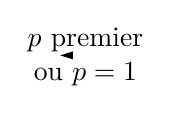
\begin{tikzpicture}[baseline=(p.base)]
\node[inner sep=0pt] (p) at (0,0) {$p$ premier};
\node[inner sep=0pt,anchor=north] at (0,-.28) {\inserted{ou $p=1$}};
% Small dark triangular mark above the addition; its guiding function is uncertain.
\fill (-.32,-.20) -- (-.16,-.15) -- (-.16,-.25) -- cycle;
\end{tikzpicture}
et $p\mid b'$ alors $\alpha'=q\alpha$
\begin{flushright}
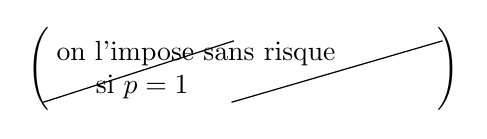
\begin{tikzpicture}[baseline=(u.base)]
\node[inner sep=0pt,anchor=west] (u) at (.22,0)
 {\rlap{on l'impose sans risque}\phantom{\deleted{on l'impose sans risque}}};
\node[inner sep=0pt,anchor=west] (v) at (.72,-.42)
 {\rlap{si $p=1$}\phantom{\deleted{si $p=1$}}};
\node[inner sep=0pt] at (0,-.20)
 {\rlap{$\Bigg($}\phantom{\deleted{$\Bigg($}}};
\node[inner sep=0pt] at (5.2,-.20)
 {\rlap{$\Bigg)$}\phantom{\deleted{$\Bigg)$}}};
% Two separate oblique cancellations over the two-line parenthesis.
\draw[line width=.45pt] (.06,-.62) -- (2.48,.16);
\draw[line width=.45pt] (2.45,-.62) -- (5.13,.16);
\end{tikzpicture}
\end{flushright}

Donc $\exists\,b_0\in\mathbb N^*$ et $\exists\,\gamma\in\mathbb N$ tel que $b'=q^\gamma b_0^q$ \margin{$q\nmid b_0$}

de plus $b_0\mid b$ et si $b=b_0 b''$ alors $b_0\mathrel{\underset{1}{\smile}}b''$ ?

De même $\exists\,a_0\in\mathbb N^*$ et $\exists\,\unsure{\zeta|\delta}\in\mathbb N$ tel que $a'=q^\zeta a_0^q$ avec $a_0\mid a$ et si $\overset{\unsure{\cdot|\prime}}{a}=a_0a''$ alors $a_0\mathrel{\underset{1}{\smile}}a''$ ?

or $a\mathrel{\underset{1}{\smile}}b\Longrightarrow a_{\deleted{\unsure{0}}}'\mathrel{\underset{1}{\smile}}b'\Longrightarrow\zeta\times\gamma=0$ (et aussi $a_0\mathrel{\underset{1}{\smile}}b_0$)

Je suppose désormais que $\zeta=0$ donc $a'=a_0^q$

\figure{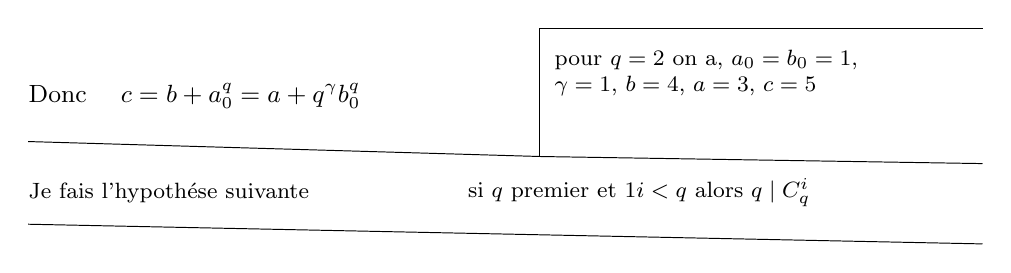
\begin{tikzpicture}[x=1cm,y=1cm]
\node[anchor=west,inner sep=0pt,font=\small] at (0,.80)
 {Donc \quad $c=b+a_0^q=a+q^\gamma b_0^q$};
\node[anchor=north west,inner sep=0pt,font=\footnotesize] at (6.68,1.43)
 {\begin{tabular}{@{}l@{}}
 pour $q=2$ on a, $a_0=b_0=1$,\\
 $\gamma=1$, $b=4$, $a=3$, $c=5$
 \end{tabular}};
% Open right border; the left edge meets the shared long upper rule.
\draw[line width=.35pt] (12.12,1.66) -- (6.50,1.66) -- (6.50,.03);
\draw[line width=.35pt] (0,.22) -- (6.50,.03) -- (12.12,-.06);
\node[anchor=west,inner sep=0pt,font=\footnotesize] at (0,-.43)
 {Je fais l'hypothése suivante};
\node[anchor=west,inner sep=0pt,font=\footnotesize] at (5.58,-.43)
 {si $q$ premier et $1\leqslant i<q$ alors $q\mid C_q^i$};
\draw[line width=.35pt] (0,-.83) -- (12.12,-1.08);
\end{tikzpicture}}
alors Si $q\geqslant3$ et $q\alpha-\alpha'\geqslant2$ \deleted{\unsure{alors}} on a \inserted{$p=q,\ {\unsure{a|\alpha}}'=\gamma$}
\[
\begin{aligned}
(1)\ \Longrightarrow\quad
 &\deleted{\unsure{p^{2}|p}}q^2\mid q\,a^{q-1}\quad
 
\begin{tikzpicture}[baseline=(d.base)]
 \node[inner sep=0pt] (d) at (0,0)
  {\rlap{ou $p=1$}\phantom{\deleted{ou $p=1$}}};
 \draw[line width=.45pt] (d.west) -- (d.east)
  .. controls +(0.22,-.04) and +(0.22,-.06) ..
  ([yshift=-2pt]d.east) -- ([yshift=-2pt]d.west);
 \end{tikzpicture}
\quad
% Faint residual strokes and points in the interline gap; no character is supplied.
\begin{tikzpicture}[baseline=-.05cm,x=1cm,y=1cm]
\draw[gray,line width=.35pt] (0,.12) .. controls (.10,.02) and (.18,-.02) .. (.31,.02);
\draw[gray,line width=.35pt] (.21,.13) -- (.27,.10);
\draw[gray,line width=.35pt] (.34,.02) .. controls (.40,.17) and (.42,.26) .. (.52,.24);
\draw[gray,line width=.35pt] (.49,.15) -- (.64,.14);
\fill[gray] (.58,.31) circle (.5pt);
\fill[gray] (.64,.04) circle (.45pt);
\fill[gray] (.69,-.02) circle (.45pt);
\end{tikzpicture}\\[.8ex]
\Longrightarrow\quad
 &q\mid a^{q-1}\quad
 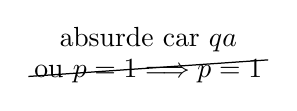
\begin{tikzpicture}[baseline=(d.base)]
 \node[inner sep=0pt] (d) at (0,0)
  {\rlap{ou $p=1\Longrightarrow p=1$}\phantom{\deleted{ou $p=1\Longrightarrow p=1$}}};
 \draw[line width=.45pt] ([xshift=-2pt,yshift=-2pt]d.west)
  -- ([xshift=2pt,yshift=4pt]d.east);
 \node[inner sep=0pt,anchor=south] at (0,.23)
  {\inserted{absurde car $q\nmid a$}};
 \end{tikzpicture}
\end{aligned}
\]
Donc $\gamma=0$ ou $\gamma=$
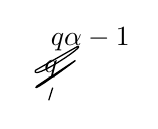
\begin{tikzpicture}[baseline=(q.base)]
\node[inner sep=0pt] (q) at (0,0)
 {\rlap{$q$}\phantom{\deleted{$q$}}};
% The live entry is physically raised above and to the right of the cancelled q.
\node[inner sep=0pt,anchor=south west] at (-.01,.22) {$q\alpha-1$};
\draw[line width=.45pt] (-.20,-.02) -- (.33,.28)
 .. controls (.48,.32) and (-.26,-.17) .. (-.20,-.02);
\draw[line width=.45pt] (-.18,-.22) -- (.30,.10)
 .. controls (.39,.16) and (-.29,-.34) .. (-.18,-.22);
\draw[line width=.45pt] (.02,-.24) -- (-.03,-.40);
\end{tikzpicture}
(sous réserve que l'hypothése est vraie)%
\margin{\begin{tikzpicture}[baseline=(n.base)]
\node[inner sep=0pt,text width=.85\marginparwidth] (n)
 {C'est peut-être interessant car ici $2$ est mis à part dans
 \(\mathord{\overset{\scriptscriptstyle\unsure{/}}{\vphantom{l}}}\)l'ensemble des nombres premiers};
% Small detached rising stroke before l'ensemble: role and hand unresolved.
% Return arrow rises at the right from the final parenthesis toward this note.
\fill ([xshift=.07cm,yshift=-.47cm]n.south east) circle(.022cm);
\draw ([xshift=.15cm,yshift=-.47cm]n.south east) -- ([xshift=.31cm,yshift=-.47cm]n.south east)
 -- ([xshift=.35cm,yshift=-.16cm]n.north east)
 .. controls([xshift=.35cm,yshift=-.03cm]n.north east) and([xshift=.19cm,yshift=-.01cm]n.north east)
 .. ([xshift=.06cm,yshift=.01cm]n.north east);
\draw ([xshift=.19cm,yshift=.14cm]n.north east) .. controls([xshift=.00cm,yshift=.04cm]n.north east) and([xshift=-.01cm,yshift=-.06cm]n.north east) .. ([xshift=.15cm,yshift=-.10cm]n.north east);
\end{tikzpicture}}
% archive sheet number: 7

\scanpage{10}
% Consolidated by root from three independent readings and seventeen adjudication crops.
% crop-candidate: scan 10
\figure{%
\begin{tikzpicture}[x=.0056cm,y=-.0056cm,line cap=round,line join=round,line width=.57pt,
 every node/.style={font=\scriptsize,inner sep=1pt}]
% Upper row. Coordinates follow the scans, with y increasing toward the foot.
\draw (118,180) .. controls (96,175) and (65,165) .. (63,146) .. controls (60,125) and (74,98) .. (94,68) .. controls (114,54) and (139,53) .. (158,62) .. controls (185,75) and (200,102) .. (186,137) .. controls (174,168) and (147,184) .. (118,180) -- cycle;
\draw (80,83) .. controls (88,71) and (96,67) .. (99,65);
\draw (136,55) .. controls (127,87) and (124,146) .. (117,181);
\draw (318,164) .. controls (303,149) and (280,133) .. (288,110) .. controls (294,84) and (305,65) .. (324,65) .. controls (344,61) and (369,61) .. (385,78) .. controls (402,97) and (402,127) .. (387,146) .. controls (369,166) and (333,176) .. (318,164) -- cycle;
\draw (304,85)--(313,65) (292,83) .. controls (303,69) and (310,78) .. (316,72);
\draw (359,63) .. controls (347,100) and (337,144) .. (319,163);
\draw (386,75) .. controls (376,99) and (355,139) .. (359,165);
\draw (528,88) .. controls (548,68) and (579,74) .. (590,94) .. controls (606,122) and (591,152) .. (572,164) .. controls (549,174) and (523,169) .. (512,155) .. controls (495,128) and (504,101) .. (528,88) -- cycle;
\draw (505,107) .. controls (512,94) and (526,94) .. (530,85);
\draw (527,88) -- (544,125) -- (563,157);
\draw (512,158) -- (544,125) -- (579,82);
\fill (545,125) circle[radius=7.5];
\node at (568,39) {OK};
\draw (714,165) .. controls (692,138) and (707,102) .. (741,82) .. controls (763,71) and (805,69) .. (824,85) .. controls (845,101) and (838,140) .. (811,169) .. controls (783,190) and (740,190) .. (714,165) -- cycle;
\draw (750,82) .. controls (741,112) and (733,154) .. (716,171);
\draw (789,74) .. controls (771,116) and (760,159) .. (758,188);
\draw (821,83) .. controls (812,113) and (798,150) .. (809,171);
\draw (774,82) -- (788,74);
\draw (877,167) .. controls (874,143) and (884,111) .. (899,102) .. controls (914,94) and (943,93) .. (957,104) .. controls (971,119) and (978,145) .. (968,163) .. controls (951,183) and (921,193) .. (898,188) .. controls (882,184) and (875,177) .. (877,167) -- cycle;
\draw (899,101) .. controls (909,128) and (902,148) .. (877,166);
\draw (934,99) .. controls (946,117) and (947,134) .. (977,137);
\draw (898,186) .. controls (925,163) and (946,151) .. (968,162);
\draw (925,98)--(927,104) (934,98)--(940,106);
\draw (1007,168) .. controls (1007,137) and (1016,107) .. (1031,102) .. controls (1052,96) and (1065,106) .. (1066,128) .. controls (1065,157) and (1048,186) .. (1027,195) .. controls (1016,201) and (1009,184) .. (1007,168) -- cycle;
\draw (1015,118) -- (1031,130) -- (1063,132) (1008,170) -- (1032,129) -- (1057,103);
\draw (1015,194) .. controls (1031,167) and (1054,156) .. (1054,176);
\fill (1033,130) circle[radius=5.3];
\draw (1038,111)--(1055,103);
\draw (1089,170) .. controls (1094,140) and (1114,106) .. (1137,93) .. controls (1161,77) and (1199,88) .. (1222,101) .. controls (1246,124) and (1228,161) .. (1207,184) .. controls (1180,207) and (1144,214) .. (1121,202) .. controls (1102,193) and (1091,184) .. (1089,170) -- cycle;
\draw (1086,171) -- (1137,135) -- (1167,113) -- (1196,92);
\draw (1119,103) -- (1138,135) .. controls (1151,149) and (1170,178) .. (1184,195);
\draw (1156,86) .. controls (1161,103) and (1168,122) .. (1179,137) .. controls (1195,152) and (1201,165) .. (1217,172);
\draw[line width=3pt] (1138,135) -- (1167,113);
\node at (1153,55) {OK};
\draw (1306,198) .. controls (1298,178) and (1312,140) .. (1333,113) .. controls (1351,93) and (1383,82) .. (1400,89) .. controls (1420,98) and (1435,120) .. (1430,147) .. controls (1413,188) and (1379,216) .. (1344,216) .. controls (1326,214) and (1312,207) .. (1306,198) -- cycle;
\draw (1317,195)--(1397,89) (1328,115)--(1425,174) (1297,172) .. controls (1340,167) and (1385,161) .. (1436,139);
\fill (1338,166)--(1363,135)--(1394,153)--cycle;
\draw[line width=2pt] (1376,90) .. controls (1385,86) and (1397,86) .. (1404,94);
\node at (1376,52) {OK};
\draw (1490,75) .. controls (1477,75) and (1450,148) .. (1446,194) .. controls (1442,229) and (1454,246) .. (1486,240);
\node at (1495,165) {ou};
\draw (1554,177) .. controls (1552,150) and (1562,112) .. (1579,106) .. controls (1599,99) and (1624,111) .. (1633,135) .. controls (1642,163) and (1621,194) .. (1600,205) .. controls (1579,218) and (1555,209) .. (1554,177) -- cycle;
\draw (1566,129) .. controls (1578,149) and (1590,162) .. (1618,175);
\draw (1583,104) .. controls (1582,132) and (1587,174) .. (1597,205);
\draw (1568,206)--(1613,107);
\draw (1567,184) .. controls (1567,196) and (1567,206) .. (1571,209);
\draw[line width=1pt] (1592,178) .. controls (1591,196) and (1590,217) .. (1587,238);
\fill (1587,159) circle[radius=6.5];
% Detached dark fragments beside the lower descending stroke; role uncertain.
\draw[line width=.7pt] (1596,174)--(1595,180) (1595,182)--(1593,187);
\fill (1584,198) circle[radius=1.2]; \fill (1598,226) circle[radius=1.2];
\draw[opacity=.45] (1548,116) .. controls (1562,103) and (1574,101) .. (1584,102);
\draw (1632,96) .. controls (1647,66) and (1657,114) .. (1649,157) .. controls (1641,212) and (1624,259) .. (1606,273);
\draw (759,202) .. controls (780,226) and (799,220) .. (828,212) .. controls (843,208) and (846,205) .. (846,217) .. controls (872,197) and (918,220) .. (949,210) -- (944,207);
\draw[line width=.55pt] (746,274) .. controls (747,244) and (777,229) .. (821,226) .. controls (863,222) and (910,214) .. (923,230) .. controls (940,253) and (888,293) .. (840,300) .. controls (787,310) and (751,304) .. (746,282) -- cycle;
\draw[line width=.7pt] (949,271) .. controls (947,245) and (987,240) .. (1015,235) .. controls (1044,226) and (1072,217) .. (1068,255) .. controls (1064,295) and (1053,303) .. (1014,305) .. controls (969,310) and (951,299) .. (949,271) -- cycle;
\node[inner sep=0pt] at (121,235) {\begin{minipage}{75pt}
\diagram{\begin{tikzcd}[ampersand replacement=\&,column sep=4pt,row sep=0pt,cells={nodes={inner sep=0pt,outer sep=0pt}}]
\bullet
\end{tikzcd}}
\end{minipage}};
\node[inner sep=0pt] at (325,236) {\begin{minipage}{75pt}
\diagram{\begin{tikzcd}[ampersand replacement=\&,column sep=4.7pt,row sep=0pt,cells={nodes={inner sep=0pt,outer sep=0pt}}]
\bullet \& \bullet
\end{tikzcd}}
\end{minipage}};
\node[inner sep=0pt] at (533,233) {\begin{minipage}{75pt}
\diagram{\begin{tikzcd}[ampersand replacement=\&,column sep=13pt,row sep=0pt,cells={nodes={inner sep=0pt,outer sep=0pt}}]
\vphantom{\bullet}\arrow[r,dash,line width=.65pt,start anchor=center,end anchor=center,shorten <=1pt,shorten >=1pt] \& \vphantom{\bullet}
\end{tikzcd}}
\end{minipage}};
\node[inner sep=0pt] at (852,253) {\begin{minipage}{75pt}
\diagram{\begin{tikzcd}[ampersand replacement=\&,column sep=8pt,row sep=0pt,cells={nodes={inner sep=0pt,outer sep=0pt}}]
\bullet \& \bullet \& \bullet
\end{tikzcd}}
\end{minipage}};
\node[inner sep=0pt] at (1009,262) {\begin{minipage}{75pt}
\diagram{\begin{tikzcd}[ampersand replacement=\&,column sep=4pt,row sep=0pt,cells={nodes={inner sep=0pt,outer sep=0pt}}]
\vphantom{\bullet}\arrow[r,dash,line width=.65pt,start anchor=center,end anchor=center,shorten <=1pt,shorten >=1pt] \&[5.2pt] \vphantom{\bullet} \&[-2pt] \bullet
\end{tikzcd}}
\end{minipage}};
\node[inner sep=0pt] at (1152,251) {\begin{minipage}{75pt}
\diagram{\begin{tikzcd}[ampersand replacement=\&,column sep=8.3pt,row sep=0pt,cells={nodes={inner sep=0pt,outer sep=0pt}}]
\bullet\arrow[r,dash,line width=.65pt,start anchor=center,end anchor=center,shorten <=1pt,shorten >=1pt] \& \unsure{\bullet|\circ}\arrow[r,dash,line width=.65pt,start anchor=center,end anchor=center,shorten <=2.7pt,shorten >=1pt] \& \bullet
\end{tikzcd}}
\end{minipage}};
\node[inner sep=0pt] at (1326,262) {\begin{minipage}{75pt}
\diagram{\begin{tikzcd}[ampersand replacement=\&,column sep=1.2pt,row sep=2.0pt,cells={nodes={inner sep=0pt,outer sep=0pt}}]
{} \& \bullet\arrow[dl,dash,line width=.65pt]\arrow[dr,dash,line width=.65pt] \& {}\\
\bullet\arrow[rr,dash,line width=.65pt] \& {} \& \bullet
\end{tikzcd}}
\end{minipage}};
% Two small, detached ink traces near the upper edge.
% Detached upper-edge marks: their hand and function remain undetermined.
\draw[opacity=.65,line width=.55pt] (1018,26) .. controls (1020,31) and (1023,32) .. (1025,27);
\draw[opacity=.65,line width=.55pt] (1037,29)--(1037,26) .. controls (1040,28) and (1043,28) .. (1046,25)--(1046,28);
% Middle row, left group.
\draw (116,390) .. controls (129,357) and (164,337) .. (200,327) .. controls (226,322) and (254,320) .. (272,326) .. controls (307,338) and (328,377) .. (326,413) .. controls (324,455) and (301,485) .. (265,500) .. controls (239,512) and (207,515) .. (184,510) .. controls (147,506) and (125,480) .. (116,455) .. controls (111,433) and (112,411) .. (116,390) -- cycle;
\draw (122,399) .. controls (122,392) and (126,388) .. (131,388);
\draw (154,353) .. controls (158,379) and (146,454) .. (128,472);
\draw (205,327) .. controls (203,354) and (205,404) .. (201,431) .. controls (197,465) and (193,491) .. (191,513);
\draw (270,324) .. controls (258,366) and (252,404) .. (253,433) .. controls (252,456) and (256,486) .. (263,501);
\draw (311,367) .. controls (296,393) and (290,441) .. (305,475);
\draw[opacity=.2] (192,503)--(195,556);
\draw (400,505) .. controls (378,492) and (374,467) .. (377,444) .. controls (382,413) and (403,377) .. (420,364) .. controls (441,342) and (462,334) .. (482,340) .. controls (514,337) and (544,366) .. (542,403) .. controls (543,444) and (508,491) .. (484,503) .. controls (462,516) and (428,521) .. (400,505) -- cycle;
\draw (419,365) .. controls (426,377) and (409,469) .. (400,503);
\draw (482,343) .. controls (461,390) and (451,446) .. (449,510);
\draw (517,356) .. controls (502,397) and (484,451) .. (481,501);
\draw[line width=1.6pt] (406,503) .. controls (423,481) and (428,504) .. (433,517);
\draw (433,512)--(434,519) (448,491)--(447,513) (456,346)--(482,340);
\draw (568,459) .. controls (563,432) and (570,399) .. (581,379) .. controls (594,358) and (612,345) .. (640,352) .. controls (665,358) and (685,385) .. (687,411) .. controls (693,446) and (680,490) .. (647,519) .. controls (636,523) and (624,523) .. (609,524) .. controls (590,517) and (571,499) .. (568,480) -- cycle;
\draw (598,359) .. controls (613,387) and (599,433) .. (567,459);
\draw (645,353) .. controls (653,386) and (676,407) .. (693,410);
\draw (570,480) .. controls (590,487) and (605,503) .. (610,524);
\draw[line width=1pt] (644,519) .. controls (647,504) and (665,473) .. (682,462);
\draw[line width=1.8pt] (684,395) .. controls (697,432) and (683,488) .. (651,516);
\draw (178,557) .. controls (177,574) and (221,577) .. (266,570) .. controls (311,564) and (361,554) .. (376,584) .. controls (378,560) and (416,560) .. (439,563) .. controls (497,573) and (539,558) .. (631,549);
\fill (733,427) circle[radius=2]; \fill (713,443) circle[radius=1.1];
% Middle row, right group.
\draw (778,444) .. controls (795,393) and (841,368) .. (889,367) .. controls (926,365) and (959,385) .. (977,414) .. controls (1001,449) and (966,489) .. (944,514) .. controls (923,544) and (901,563) .. (874,562) .. controls (842,564) and (800,553) .. (774,526) .. controls (774,509) and (771,472) .. (778,444) -- cycle;
\draw (772,446) .. controls (815,439) and (889,422) .. (947,388);
\draw (790,536) -- (854,425) -- (891,367);
\draw (778,464) .. controls (801,466) and (800,495) .. (777,509);
\draw (909,368) .. controls (910,392) and (925,388) .. (937,375);
\draw (774,517) .. controls (783,516) and (781,535) .. (791,536);
\fill (855,425) circle[radius=7.6];
\draw (990,500) .. controls (989,465) and (1002,432) .. (1026,409) .. controls (1047,386) and (1072,381) .. (1088,394) .. controls (1114,409) and (1110,444) .. (1104,473) .. controls (1098,508) and (1073,550) .. (1052,568) .. controls (1023,582) and (1009,571) .. (1000,548) .. controls (994,529) and (990,511) .. (990,500) -- cycle;
\draw (1021,412) .. controls (1043,438) and (1062,481) .. (1078,517);
\draw (998,534) .. controls (1023,505) and (1065,431) .. (1091,399);
\draw (998,456) .. controls (1018,463) and (1009,490) .. (991,501);
\draw (1015,570) .. controls (1034,544) and (1052,547) .. (1057,562);
\fill (1053,458) ellipse[x radius=6.8,y radius=9];
\draw (1133,512) .. controls (1136,476) and (1157,427) .. (1183,402) .. controls (1209,376) and (1248,380) .. (1268,395) .. controls (1296,420) and (1293,459) .. (1285,493) .. controls (1274,530) and (1241,562) .. (1208,571) .. controls (1171,582) and (1146,555) .. (1137,534) .. controls (1133,523) and (1132,516) .. (1133,512) -- cycle;
\draw (1172,411) -- (1207,472) .. controls (1222,498) and (1233,526) .. (1243,551);
\draw (1144,552) .. controls (1161,534) and (1218,450) .. (1266,395);
\draw (1155,453) .. controls (1175,478) and (1159,506) .. (1133,523);
\draw (1159,444) .. controls (1166,453) and (1181,440) .. (1171,428);
\fill (1207,472) circle[radius=7.3];
\draw (1285,514) .. controls (1291,476) and (1311,437) .. (1337,415) .. controls (1356,400) and (1381,409) .. (1391,423) .. controls (1417,463) and (1404,507) .. (1384,535) .. controls (1369,559) and (1349,583) .. (1327,588) .. controls (1306,591) and (1288,575) .. (1284,550) .. controls (1281,536) and (1282,525) .. (1285,514) -- cycle;
\draw (1315,444) -- (1342,491) -- (1368,559);
\draw (1290,564) .. controls (1307,552) and (1355,466) .. (1388,423);
\draw (1299,575) .. controls (1317,554) and (1335,524) .. (1347,555) -- (1353,570);
\draw (1312,585) .. controls (1328,561) and (1340,561) .. (1340,582);
\fill (1343,492) circle[radius=6.6];
\fill (1307,505) .. controls (1310,497) and (1314,496) .. (1318,483) .. controls (1324,477) and (1329,500) .. (1324,509) .. controls (1317,520) and (1305,515) .. (1307,505) -- cycle;
% Undetermined trace: pale intervals separate the darker parts of this upper extension.
\draw[opacity=.22] (1328,433) .. controls (1330,406) and (1335,357) .. (1341,329);
\draw[line width=.65pt] (1340,332)--(1339,339) (1338,343) .. controls (1336,351) and (1337,359) .. (1335,365);
\draw[line width=.55pt] (1333,382)--(1332,389) (1331,398)--(1330,403) (1329,411)--(1327,432);
\draw[line width=1.8pt] (1327,436) .. controls (1335,425) and (1340,416) .. (1349,418);
\draw (793,583) .. controls (822,621) and (923,616) .. (981,613) .. controls (1025,612) and (1060,623) .. (1079,622) .. controls (1090,628) and (1095,637) .. (1102,649) .. controls (1114,632) and (1127,626) .. (1138,621) .. controls (1220,627) and (1280,619) .. (1348,616) .. controls (1354,610) and (1360,601) .. (1364,592);
\draw (1004,605) .. controls (1015,626) and (1050,615) .. (1069,622) (1167,622) -- (1204,630);
\node[font=\bfseries\small] at (539,658) {?};
\node[inner sep=0pt] at (373,646) {\begin{minipage}{85pt}
\diagram{\begin{tikzcd}[ampersand replacement=\&,column sep=7pt,row sep=0pt,cells={nodes={inner sep=0pt,outer sep=0pt}}]
\bullet \& \bullet \& \bullet \& \bullet
\end{tikzcd}}
\end{minipage}};
\node[inner sep=0pt] at (848,648) {\begin{minipage}{85pt}
\diagram{\begin{tikzcd}[ampersand replacement=\&,column sep=11.1pt,row sep=0pt,cells={nodes={inner sep=0pt,outer sep=0pt}}]
\vphantom{\bullet}\arrow[r,dash,line width=.65pt,start anchor=center,end anchor=center,shorten <=1pt,shorten >=1pt] \& \vphantom{\bullet} \& \bullet \& \bullet
\end{tikzcd}}
\end{minipage}};
% Lower row.
\draw[opacity=.22,line width=.4pt] (1518,375) .. controls (1540,374) and (1561,405) .. (1524,401);
\fill[opacity=.75] (1566,580) circle[radius=1.25]; \fill[opacity=.65] (1561,587) circle[radius=1];
\node at (201,691) {OK};
\draw (123,811) .. controls (135,770) and (168,740) .. (208,726) .. controls (239,716) and (275,725) .. (304,749) .. controls (339,775) and (354,809) .. (350,840) .. controls (347,879) and (314,935) .. (279,960) .. controls (257,972) and (226,969) .. (198,968) .. controls (162,965) and (130,943) .. (121,913) .. controls (114,887) and (118,844) .. (123,811) -- cycle;
\draw (124,893) .. controls (149,863) and (184,800) .. (219,718);
\draw (125,813) -- (194,773) .. controls (223,757) and (257,743) .. (274,727);
\draw (198,968) -- (298,838) -- (340,790);
\draw (277,965) .. controls (283,927) and (291,876) .. (298,839) .. controls (303,812) and (307,781) .. (310,754);
\fill (194,773) circle[radius=7.5]; \fill (299,838) circle[radius=7];
\draw[opacity=.14] (252,825)--(256,825) (259,825)--(264,826) (267,826)--(271,826) (274,827)--(278,827);
\draw[opacity=.4] (278,827)--(293,828);
% State remains uncertain: diagonal cancellation | hatching. Only the visible diagonal paths are inked.
\node[inner sep=0pt,outer sep=0pt,anchor=center] at (548,820) {\unsure{\rlap{\hbox{\begin{tikzpicture}[x=.0056cm,y=-.0056cm,line cap=round,line join=round,line width=.57pt,color=black]
\path[use as bounding box] (450,714) rectangle (646,926);
\draw (460,830) .. controls (473,785) and (509,749) .. (541,731) .. controls (566,724) and (595,741) .. (613,754) .. controls (645,781) and (638,817) .. (626,842) .. controls (605,883) and (571,914) .. (538,917) .. controls (508,924) and (480,912) .. (462,889) .. controls (452,874) and (454,848) .. (460,830) -- cycle;
\draw (474,789) -- (612,754) (461,891) -- (547,729) (556,729) .. controls (578,778) and (605,805) .. (628,838);
% Repeated diagonal cancellation strokes in this disk.
\draw (535,717) .. controls (526,729) and (457,833) .. (461,835) .. controls (470,838) and (538,725) .. (537,729) .. controls (515,764) and (465,860) .. (470,865) .. controls (476,870) and (554,747) .. (565,747) .. controls (549,777) and (493,861) .. (493,865) .. controls (504,870) and (569,753) .. (585,751) .. controls (557,783) and (513,860) .. (518,866) .. controls (526,877) and (601,791) .. (614,798) .. controls (618,801) and (589,843) .. (563,892) .. controls (554,907) and (560,914) .. (572,923);
% Small pale descending trace and dark tip at the lower-left outline.
\draw[opacity=.16,line width=.4pt] (490,861) .. controls (488,885) and (490,901) .. (491,915);
\draw[line width=.55pt] (491,912)--(490,920);
\end{tikzpicture}}}\phantom{\deleted{\hbox{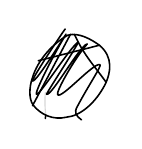
\begin{tikzpicture}[x=.0056cm,y=-.0056cm,line cap=round,line join=round,line width=.57pt,color=black]
\path[use as bounding box] (450,714) rectangle (646,926);
\draw (460,830) .. controls (473,785) and (509,749) .. (541,731) .. controls (566,724) and (595,741) .. (613,754) .. controls (645,781) and (638,817) .. (626,842) .. controls (605,883) and (571,914) .. (538,917) .. controls (508,924) and (480,912) .. (462,889) .. controls (452,874) and (454,848) .. (460,830) -- cycle;
\draw (474,789) -- (612,754) (461,891) -- (547,729) (556,729) .. controls (578,778) and (605,805) .. (628,838);
% Repeated diagonal cancellation strokes in this disk.
\draw (535,717) .. controls (526,729) and (457,833) .. (461,835) .. controls (470,838) and (538,725) .. (537,729) .. controls (515,764) and (465,860) .. (470,865) .. controls (476,870) and (554,747) .. (565,747) .. controls (549,777) and (493,861) .. (493,865) .. controls (504,870) and (569,753) .. (585,751) .. controls (557,783) and (513,860) .. (518,866) .. controls (526,877) and (601,791) .. (614,798) .. controls (618,801) and (589,843) .. (563,892) .. controls (554,907) and (560,914) .. (572,923);
% Small pale descending trace and dark tip at the lower-left outline.
\draw[opacity=.16,line width=.4pt] (490,861) .. controls (488,885) and (490,901) .. (491,915);
\draw[line width=.55pt] (491,912)--(490,920);
\end{tikzpicture}}}}}};
\draw (666,836) .. controls (669,808) and (686,789) .. (706,785) .. controls (725,782) and (746,786) .. (755,803) .. controls (773,824) and (771,857) .. (758,880) .. controls (746,903) and (728,917) .. (706,910) .. controls (683,903) and (660,871) .. (666,836) -- cycle;
\draw (707,786) -- (694,902) (747,789) .. controls (739,827) and (735,869) .. (729,906);
\draw (666,840)--(767,844);
\draw[line width=3.4pt] (699,838)--(737,842);
\draw (718,786) .. controls (715,814) and (733,813) .. (737,789);
\draw (797,850) .. controls (804,822) and (821,801) .. (839,798) .. controls (864,797) and (876,815) .. (881,839) .. controls (890,866) and (876,895) .. (860,910) .. controls (841,926) and (822,917) .. (809,905) .. controls (796,890) and (792,870) .. (797,850) -- cycle;
\draw (827,805) .. controls (823,843) and (819,878) .. (816,915);
\draw (862,805) .. controls (858,842) and (854,879) .. (852,914);
\draw (799,861)--(890,859); \draw[line width=2.8pt] (820,857)--(853,857);
\draw (874,818) .. controls (868,841) and (868,848) .. (885,850);
\draw (543,948) .. controls (573,976) and (607,963) .. (665,954) .. controls (706,949) and (731,945) .. (741,967) .. controls (744,947) and (789,945) .. (826,944) .. controls (864,943) and (881,941) .. (899,937) -- (898,931);
\node at (1156,724) {OK};
\draw (1004,849) .. controls (1005,815) and (1033,783) .. (1069,769) .. controls (1101,757) and (1134,762) .. (1150,787) .. controls (1172,815) and (1183,855) .. (1165,903) .. controls (1149,943) and (1125,964) .. (1109,969) .. controls (1072,976) and (1040,970) .. (1024,945) .. controls (1004,913) and (997,879) .. (1004,849) -- cycle;
\draw[opacity=.65] (1006,850) .. controls (1002,859) and (1003,869) .. (1009,874);
\draw (1012,924) .. controls (1029,875) and (1050,817) .. (1070,770);
\draw (1011,808) .. controls (1055,804) and (1125,796) .. (1156,788);
\draw (1101,764) .. controls (1110,780) and (1116,791) .. (1120,798) -- (1174,881);
\draw (1109,967) .. controls (1127,926) and (1154,855) .. (1172,823);
\draw[line width=2.7pt] (1056,802)--(1119,794);
\draw[line width=3.7pt] (1118,795)--(1158,853);
% Detached short dark trace below the broad segment; role and hand undetermined.
\draw[line width=.55pt] (1166,875)--(1165,879);
% Detached pale irregular patch; hand, origin and role remain undetermined.
\filldraw[fill opacity=.10,draw opacity=.16,line width=.3pt]
(1629,793) .. controls (1629,790) and (1631,788) .. (1635,788)
--(1636,786)--(1640,790)--(1645,792)
.. controls (1649,795) and (1648,799) .. (1646,802)
--(1643,803)--(1640,806)--(1637,808)--(1634,804)--(1630,804)
.. controls (1627,801) and (1627,797) .. (1629,793)--cycle;
% Two faint, angular lines at the foot, crossing the last graph and continuing at the right.
\draw[opacity=.55] (1010,975) .. controls (1027,995) and (1035,1030) .. (1044,1050) .. controls (1053,1074) and (1061,1090) .. (1075,1089);
\draw[line width=1.5pt] (1041,1036) .. controls (1052,1070) and (1060,1090) .. (1074,1088);
\draw[opacity=.16] (1073,1088) .. controls (1108,1087) and (1162,1076) .. (1214,1064) -- (1288,985);
\draw[opacity=.5] (1215,1073)--(1237,1044) (1246,1033)--(1261,1014) (1278,996)--(1289,982);
\draw[opacity=.22] (1345,934) .. controls (1353,954) and (1350,994) .. (1358,1009) -- (1372,1014);
\draw[line width=1.9pt] (1373,1014) .. controls (1390,1025) and (1430,1037) .. (1458,1048) -- (1484,1054) -- (1500,1036);
\draw[opacity=.5] (1487,1054)--(1581,957);
\draw[opacity=.23] (1568,905) .. controls (1572,924) and (1571,943) .. (1581,957);
\node[inner sep=0pt] at (222,1035) {\begin{minipage}{94pt}
\diagram{\begin{tikzcd}[ampersand replacement=\&,column sep=5.2pt,row sep=0pt,cells={nodes={inner sep=0pt,outer sep=0pt}}]
\unsure{\circ|\bullet}\arrow[r,dash,line width=.65pt,start anchor=center,end anchor=center,shorten <=1pt,shorten >=1pt] \& \circ \& \hspace{3.3pt} \& \bullet\arrow[r,dash,line width=.65pt,start anchor=center,end anchor=center,shorten <=1pt,shorten >=1pt] \& \bullet
\end{tikzcd}}
\end{minipage}};
\node[inner sep=0pt] at (563,1026) {\begin{minipage}{94pt}
\diagram{\begin{tikzcd}[ampersand replacement=\&,column sep=7pt,row sep=0pt,cells={nodes={inner sep=0pt,outer sep=0pt}}]
\unsure{\circ|\bullet}\arrow[r,dash,line width=.65pt,start anchor=center,end anchor=center,shorten <=1pt,shorten >=1pt] \& \bullet\arrow[r,dash,line width=.65pt,start anchor=center,end anchor=center,shorten <=2.7pt,shorten >=1pt] \& \bullet \& \bullet
\end{tikzcd}}
\end{minipage}};
\node[inner sep=0pt] at (1075,1032) {\begin{minipage}{94pt}
\diagram{\begin{tikzcd}[ampersand replacement=\&,column sep=9pt,row sep=0pt,cells={nodes={inner sep=0pt,outer sep=0pt}}]
\unsure{\bullet|\circ}\arrow[r,dash,line width=.65pt,start anchor=center,end anchor=center,shorten <=1pt,shorten >=1pt] \& \bullet\arrow[r,dash,line width=.65pt,start anchor=center,end anchor=center,shorten <=1pt,shorten >=1pt] \& \bullet\arrow[r,dash,line width=.65pt,start anchor=center,end anchor=center,shorten <=1pt,shorten >=1pt] \& \bullet
\end{tikzcd}}
\end{minipage}};

% Hook projecting above/right of the uncertain middle vertex under upper disk 7.
\draw[line width=.65pt] (1153,251) .. controls (1154,245) and (1159,246) .. (1163,252);
% Tiny detached spot just above the outer lower arch in the last middle disk.
\fill (1314,543) circle[radius=1.4];
% Pale detached marks; hand, purpose, and surface origin remain undetermined.
% Above upper disk4 the short course is supported; its faint lower continuation is unresolved.
\draw[opacity=.14,line width=.4pt] (416,241) .. controls (425,250) and (426,260) .. (421,266) .. controls (416,274) and (410,275) .. (403,275);
\draw[opacity=.16,line width=.4pt] (784,42) .. controls (784,49) and (785,55) .. (787,62);
\draw[opacity=.4,line width=.4pt] (786,56)--(786,59);
\draw[opacity=.16,line width=.35pt] (369,743) .. controls (379,751) and (390,762) .. (405,778) -- (415,786);
\draw[opacity=.25,line width=.4pt] (377,751)--(384,758) (390,764)--(393,767);
\draw[opacity=.14,line width=.4pt] (1567,352) .. controls (1570,358) and (1576,360) .. (1580,362);
% Pale diagonal inside the right angular trace, with independently detached lower dash.
% Only the short supported course is reproduced; a farther upper continuation remains unresolved.
\node[anchor=north west,inner sep=0pt,outer sep=0pt] at (1438,978) {\unsure{\hbox{\begin{tikzpicture}[x=.0056cm,y=-.0056cm,line cap=round,color=black]
\path[use as bounding box] (1438,978) rectangle (1504,1039);
\draw[opacity=.13,line width=.4pt] (1444,1037) .. controls (1460,1018) and (1488,989) .. (1500,980);
\end{tikzpicture}}}};
\draw[opacity=.45,line width=.45pt] (1435,1084)--(1437,1093);
% Dark pieces and small detached marks around the upper-right angular-trace endpoint.
\draw[opacity=.75,line width=.45pt] (1568,908)--(1570,917);
\fill[opacity=.65] (1566,921) circle[radius=1.15];
\fill[opacity=.3] (1550,893) circle[radius=1.2];
\fill[opacity=.2] (1603,930) circle[radius=1.6];
\end{tikzpicture}}
% archive sheet number: 9

\scanpage{11}
\[
 \unsure{=|\Rightarrow}
\]
\[
 \begin{aligned}
 \mathbb P\left(
 \begin{tikzpicture}[x=.0043cm,y=-.0043cm,baseline={(0,82)},line cap=round,line join=round]
 \draw[line width=.5pt] (18,12) -- (59,76) (64,1) -- (23,78);
 \draw[line width=.5pt] (0,1) -- (30,3) (63,0) -- (76,1)
 (0,80) -- (26,78) (58,76) -- (78,77);
 \end{tikzpicture}\right)&\qquad
 P(X\times\unsure{Z|2})\overset{?}{\simeq}
 \operatorname{Hom}(\underset{\unsure{\cdot}}{\deleted{\unsure{e|\mathcal E}}Z}\times X,\mathscr E)\\
 &\qquad\mathrel{/\!/}\quad
 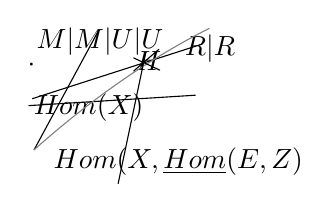
\begin{tikzpicture}[x=.011cm,y=-.011cm,baseline=(live.base),line cap=round,line join=round]
 % The cancellation paths are drawn explicitly. Invisible deleted copies retain the deletion annotation.
 \node[anchor=base west,inner sep=0] at (74,110)
 {\rlap{$\operatorname{Hom}(X)$}\phantom{$\deleted{\operatorname{Hom}(X)}$}};
 \node[inner sep=0] at (151,26)
 {$\unsure{\rlap{$M$}\phantom{\deleted{M}}|M|\rlap{$U$}\phantom{\deleted{U}}|U}$};
 \node[inner sep=0] at (207,48)
 {\rlap{$H$}\phantom{$\deleted{H}$}};
 \node[inner sep=0] at (278,34)
 {$\unsure{\rlap{$R$}\phantom{\deleted{R}}|R}$};
 \draw (69,100) -- (261,88);
 \draw (73,92) -- (269,29);
 \draw (75,151) -- (149,14);
 \draw[gray] (75,151) .. controls (120,111) and (191,54) .. (277,11);
 \draw (172,190) -- (204,38);
 \draw (190,60) -- (219,35) (190,45) -- (220,59);
 \node[inner sep=0] at (72,54) {$\unsure{\cdot}$};
 \node[anchor=base west,inner sep=0] (live) at (97,173)
 {$\operatorname{Hom}(X,\underline{\operatorname{Hom}}(\mathscr E,Z)$};
 \end{tikzpicture}\\
 \unsure{O|0}\subset\mathbb{P}(X)&\qquad
 \operatorname{Hom}(\mathscr E,\underline{\operatorname{Hom}}(X,Z))\\
 &\qquad\mathrel{/\!/}\\
 &\qquad P(\operatorname{Hom}(X,Z)
 \end{aligned}
\]
\figure{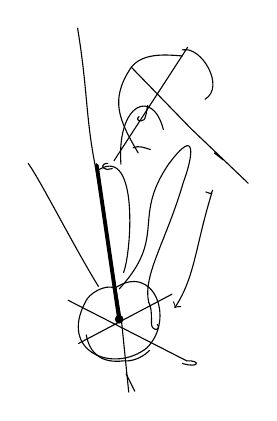
\begin{tikzpicture}[x=.011cm,y=-.011cm,line cap=round,line join=round]
\draw (63,1) .. controls (75,74) and (72,104) .. (84,163) -- (114,342) -- (122,421);
\draw[line width=1.4pt] (85,159) -- (111,337);
\draw (6,157) .. controls (22,180) and (57,250) .. (87,299);
\draw (64,365) -- (172,308) (52,315) -- (189,385);
\draw (106,301) .. controls (151,271) and (176,337) .. (143,370)
 .. controls (105,400) and (41,375) .. (72,317) .. controls (76,307) and (95,296) .. (106,301);
\fill (111,337) circle (5);
\draw (105,154) -- (190,23) (184,26) .. controls (206,21) and (234,69) .. (210,83)
 (125,46) -- (194,117) -- (260,180) (231,153) -- (221,145);
\draw (133,145) .. controls (110,106) and (100,83) .. (125,46) .. controls (139,28) and (169,32) .. (184,33);
\draw (113,158) .. controls (108,87) and (150,70) .. (162,118);
\draw (88,164) .. controls (134,137) and (125,261) .. (116,283);
\draw (111,302) .. controls (167,241) and (125,221) .. (168,158)
 .. controls (202,112) and (196,150) .. (185,179) .. controls (166,245) and (138,286) .. (145,317);
\draw[->] (218,191) .. controls (199,252) and (199,287) .. (175,324);
% Local small paths seen in the junction and disk crops; no letter or role assigned.
\draw (98,157) .. controls (90,157) and (90,163) .. (97,164) -- (103,163);
\draw (127,139) .. controls (134,136) and (140,139) .. (147,141);
\draw (144,90) .. controls (142,98) and (142,109) .. (136,108)
 .. controls (132,108) and (131,105) .. (134,103);
\draw (73,355) .. controls (77,377) and (91,388) .. (116,385)
 .. controls (128,386) and (139,380) .. (146,373);
\draw (189,385) .. controls (205,384) and (204,394) .. (184,388);
\draw (145,317) .. controls (151,329) and (146,344) .. (150,347)
 .. controls (156,352) and (158,345) .. (155,343);
\draw (119,400) -- (129,420);
\draw (211,190) -- (217,192) -- (219,188);
% crop-candidate: scan 11
\end{tikzpicture}}
\[
 \begin{aligned}
 \begin{tikzpicture}[baseline=(hom.base),line cap=round]
 \node[inner sep=0] (hom) at (0,0) {$\underline{\operatorname{Hom}}$};
 \node[inner sep=0] at (-.78,.12) {\unsure{\begin{tikzpicture}[x=.015cm,y=-.015cm]
 \draw[gray] (0,0) .. controls (3,3) and (6,5) .. (10,6);
 \draw (10,6) -- (12,6.5);
 \end{tikzpicture}}};
 \end{tikzpicture}(X,Y)&\subset P(X\times Y)\\
 \operatorname{Hom}(\begin{tikzpicture}[baseline=(z.base),line cap=round,line join=round]
 \node[inner sep=0] (z) at (0,0) {$\deleted{\unsure{t|1}}Z$};
 \node[inner sep=0] at (.17,.48) {\unsure{\begin{tikzpicture}[line cap=round,line join=round]
 \draw (0,0) -- (.08,.06) -- (.15,.03) -- (.23,.06) -- (.30,.04);
 \fill (.38,.04) circle (.012);
 \fill[gray] (.43,.03) circle (.009);
 \end{tikzpicture}}};
 \end{tikzpicture}\times X,Y)&\subset
 \underset{\text{\unsure{\begin{tikzpicture}[x=.014cm,y=-.014cm,baseline=0,line cap=round,line join=round]
 \draw (-13,0) -- (-8,1);
 \draw (-2,2) -- (0,-2) -- (3,1) -- (5,-1) -- (6,2);
 \draw (10,-1) -- (11,3);
 \end{tikzpicture}}}}{P}
 (\underset{\text{\unsure{\begin{tikzpicture}[x=.014cm,y=-.014cm,baseline=0,line cap=round]
 \fill (-8,0) circle (1.2);
 \fill[gray] (1,1) circle (1.4);
 \draw[gray] (6,2) -- (8,-1) (12,1) -- (13,-1) (15,0) -- (17,-2);
 \end{tikzpicture}}}}{Z}\times X\times Y)
 \end{aligned}
\]
\diagram{\begin{tikzcd}[ampersand replacement=\&,row sep=small,column sep=small,
 execute at end picture={
  % Retraced lower horizontal arrow shaft and extended upper head stroke.
  \draw[line width=.45pt] ([xshift=-4pt,yshift=-1pt]sxiU.west)
    .. controls ([xshift=-18pt,yshift=-5pt]sxiU.west) and ([xshift=15pt,yshift=-5pt]sxiV.east)
    .. ([xshift=4pt,yshift=-1pt]sxiV.east);
  \draw ([xshift=8pt,yshift=5pt]sxiV.east) -- ([xshift=11pt,yshift=9pt]sxiV.east);
  % Loop at the downward arrowhead, plus its two detached marks.
  \draw ([xshift=-5pt,yshift=9pt]sxiPX.north)
    .. controls ([xshift=-9pt,yshift=14pt]sxiPX.north) and ([xshift=-10pt,yshift=8pt]sxiPX.north)
    .. ([xshift=-4pt,yshift=6pt]sxiPX.north);
  \node[inner sep=0] at ([xshift=-12pt,yshift=14pt]sxiPX.north) {$\unsure{\cdot}$};
  \node[inner sep=0] at ([xshift=14pt,yshift=5pt]sxiPX.north) {$\unsure{\textcolor{gray}{\cdot}}$};
 }]
 \& {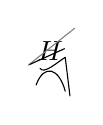
\begin{tikzpicture}[baseline=(h.base),line cap=round,line join=round]
 \node[inner sep=0] (h) at (0,0) {\rlap{$H$}\phantom{$\deleted{H}$}};
 \draw[gray] (-.28,-.18) -- (.31,.29);
 \draw (-.26,-.17) -- (.18,.03);
 \draw (-.13,-.22) .. controls (-.08,-.30) and (.09,-.14) .. (.19,-.08);
 \draw (.19,-.08) -- (.25,-.57);
 \draw (-.18,-.43) .. controls (-.08,-.16) and (.11,-.21) .. (.19,-.51);
 \end{tikzpicture}} \& \& \\
 \& {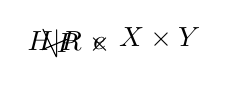
\begin{tikzpicture}[baseline=(prod.base),line cap=round,line join=round]
 \node[inner sep=0] at (-.12,0) {\rlap{$\unsure{H|R}$}\phantom{$\deleted{\unsure{H|R}}$}};
 \node[inner sep=0] (prod) at (.04,0) {$P$};
 \draw (-.27,.18) -- (-.10,-.17) (-.28,-.08) -- (.03,.05);
 \node[inner sep=0] at (.45,0) {\rlap{$e$}\phantom{$\deleted{e}$}};
 \node[inner sep=0] at (.45,-.02) {$\times$};
 \node[anchor=base west,inner sep=0] at (.69,-.04) {$X\times Y$};
 \end{tikzpicture}}
 \arrow[d,"{
\begin{tikzpicture}[baseline=(u.base),line cap=round,line join=round]
 \node[inner sep=0] (u) at (0,0)
 {\rlap{$\unsure{H|U}$}\phantom{$\deleted{\unsure{H|U}}$}};
 \draw (-.21,-.21) -- (.24,.36);
 \draw (.05,-.13) .. controls (-.03,-.45) and (.13,-.54) .. (.33,-.31);
 \end{tikzpicture}}"'] \& \&
 {\supset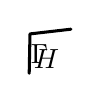
\begin{tikzpicture}[baseline=(g.base),line cap=round,line join=round]
 \node[inner sep=0] at (.09,-.04) {\rlap{$H$}\phantom{$\deleted{H}$}};
 \node[inner sep=0] (g) at (0,.03) {$\Gamma$};
 \draw[line width=1.1pt] (-.13,-.22) -- (-.12,.28) -- (.40,.34);
 \end{tikzpicture}}\arrow[dll] \\
 \& |[alias=sxiPX]| P\times X\arrow[dl] \& \& U\times_{\unsure{Y|V}}U\\
 {\begin{tikzpicture}[baseline=(p.base),line cap=round]
 \node[inner sep=0] (p) at (.29,-.25) {$P$};
 \node[inner sep=0] at (-1.03,.91) {$\unsure{\cdot}$};
 \draw[gray] (-1.11,.94) .. controls (-1.10,.92) and (-1.08,.91) .. (-1.07,.90);
 \draw (-.08,1.0) .. controls (-.06,.35) and (-.12,-.55) .. (-.09,-1.04);
 \draw (-.06,.48) .. controls (-.03,-.10) and (.02,-.67) .. (.08,-.92);
 \node[inner sep=0] at (.21,.03) {\unsure{\begin{tikzpicture}[x=.015cm,y=-.015cm,line cap=round]
 \draw[gray] (0,0) .. controls (3,-3) and (4,0) .. (3,3) -- (4,8);
 \end{tikzpicture}}};
 \end{tikzpicture}}
 \& |[alias=sxiV]| \unsure{V|W} \& \& |[alias=sxiU]| U\arrow[ll]\\
 \& \& {\begin{tikzpicture}[x=.011cm,y=-.011cm,baseline=(p.base),line cap=round]
 \node[inner sep=0,anchor=base] (p) at (0,0) {$P$};
 \draw (-42,-102) .. controls (-30,-94) and (-30,-78) .. (-22,-66);
 \draw[gray] (60,-113) -- (30,-59);
 \fill (30,-59) circle (1.2);
 \node[inner sep=0] at (2,21) {\unsure{\begin{tikzpicture}[x=.011cm,y=-.011cm,line cap=round]
 \draw[line width=.7pt] (-1,-13) .. controls (0,-4) and (1,5) .. (3,13);
 \fill (3,13) circle (1.2);
 \end{tikzpicture}}};
 \end{tikzpicture}} \&
\end{tikzcd}}
\figure{\begin{tikzpicture}[x=.011cm,y=-.011cm,line join=round,line cap=round]
% crop-candidate: scan 11
% The three bottom drawings were checked individually on the supplied halves.
\draw (13,425) -- (98,53);
\draw (98,46) -- (130,35) (139,32) -- (155,26) (164,23) -- (215,4);
\draw (215,4) -- (282,69);
\draw (282,76) -- (267,303) -- (145,352) -- (13,425);
\draw (215,4) -- (210,-3) (219,5) -- (218,-4);
\draw (13,425) -- (6,414) (267,303) -- (270,313);
\draw[line width=1.8pt] (216,8) -- (272,69) (278,226) -- (267,304) -- (147,351) -- (41,253);
\draw (209,4) .. controls (230,40) and (248,53) .. (272,68) (282,74) -- (219,0);
\draw (6,237) .. controls (47,191) and (63,184) .. (74,188)
 (3,214) -- (144,362) -- (178,405) (6,209) -- (159,358);
\draw (35,185) .. controls (-5,206) and (15,266) .. (48,309)
 .. controls (115,383) and (151,428) .. (171,406);
\draw[->] (46,199) .. controls (80,196) and (208,305) .. (184,407);
\draw (86,366) .. controls (86,389) and (188,345) .. (237,329);
\draw (319,271) -- (430,382) -- (549,389) -- (624,258) (319,271) -- (498,464) (535,454) -- (617,264);
\draw[line width=2pt] (325,275) -- (429,374) -- (556,384) -- (620,263);
\draw (319,268) -- (556,384) (361,299) -- (543,381);
\draw (501,486) .. controls (530,446) and (552,450) .. (570,357);
\draw (416,389) .. controls (421,396) and (430,396) .. (438,389);
\draw (562,388) -- (574,391) (564,398) -- (578,402);
\node[inner sep=0] at (523,276) {\unsure{\begin{tikzpicture}[x=.011cm,y=-.011cm,line cap=round]
\fill (0,0) circle (1.2); \draw[gray] (1,1) -- (3,2);
\end{tikzpicture}}};
\draw (627,259) -- (745,421);
\draw (640,291) .. controls (722,169) and (814,239) .. (883,324)
 .. controls (934,419) and (753,461) .. (678,394) .. controls (654,378) and (643,338) .. (648,316);
\draw (676,252) .. controls (710,302) and (679,351) .. (678,400)
 (705,230) .. controls (675,312) and (707,386) .. (709,416)
 (731,225) .. controls (722,312) and (765,383) .. (782,421);
\draw (783,244) -- (868,399) (815,250) .. controls (797,322) and (811,374) .. (850,416)
 (860,285) .. controls (847,342) and (824,363) .. (822,426);
\draw (684,318) -- (698,354) -- (685,337) -- (698,365)
 (811,316) -- (835,347) -- (812,328) -- (837,358) -- (813,342) -- (833,369);
\end{tikzpicture}}
% archive sheet number: 10

\scanpage{12}
% Consolidated scan012; all root crop decisions are recorded in the accompanying changes log.
% All source full-pixel coordinates and literal C contour blocks are retained.
% Editorial descriptions and alternatives appear only in comments.
\figure{\begin{tikzpicture}[x=0.0076cm,y=-0.0076cm,line join=round,line cap=round]
% C source path 01: literal block retained once.
\path[fill=black,even odd rule]
(505.5,23) -- (514,23.6) -- (529.4,34) -- (535.4,44) -- (538.4,56) -- (538.5,62) -- (536.5,67) -- (537.4,71) -- (533.6,75) -- (531.4,81)
 -- (528.7,83) -- (530,89.5) -- (528,90.4) -- (523,88.4) -- (523.3,86) -- (519,81.7) -- (515,82.7) -- (511.7,86) -- (509.7,93) -- (515,92.3)
 -- (520,88.6) -- (522.5,89) -- (522.5,90) -- (522.4,91) -- (517,94.4) -- (505,98.5) -- (496,96.4) -- (494,94.7) -- (492,96.4) -- (488.6,96)
 -- (487.7,94) -- (489.3,89) -- (483.6,76) -- (481.5,55) -- (484.3,42) -- (483.7,39) -- (486.6,34) -- (491,29.6) -- (502,23.6) -- cycle
(510,26.8) -- (506.7,29) -- (503,45.3) -- (508,46.1) -- (523.1,32) -- (518,28.6) -- cycle
(525,33.7) -- (508.7,50) -- (535,67.3) -- (536.5,58) -- (534.5,47) -- (529.3,38) -- cycle
(488,42.9) -- (486.7,44) -- (485.5,51) -- (484.7,63) -- (486,64.2) -- (495.3,57) -- (497.5,51) -- (495.4,48) -- cycle
(502,27.8) -- (492,37.3) -- (490,35.8) -- (488.7,37) -- (489.6,40) -- (497,45.3) -- (499.3,43) -- (503.3,31) -- cycle
(508,53.8) -- (500.7,57) -- (493.7,88) -- (497,93.3) -- (504,95.2) -- (506.3,93) -- (508.6,85) -- (513,79.6) -- (521,78.6) -- (527,82.3)
 -- (532.5,75) -- (532.3,72) -- (530,68.7) -- (526,71.4) -- (524.3,66) -- (521.4,63) -- cycle
(495,59.9) -- (485.7,70) -- (490,85.3) -- (491,85.3) -- (491.3,85) -- (492.3,82) -- (495.3,68) -- cycle
;
% C source path 02: literal block retained once.
\path[fill=black,even odd rule]
(318.5,47) -- (334,46.5) -- (343,47.6) -- (367,55.6) -- (391,69.6) -- (398,74.6) -- (409,85.5) -- (415.4,93) -- (423.4,106) -- (431.4,129)
 -- (431.7,135) -- (438,137.6) -- (439.4,140) -- (439.4,141) -- (439,141.4) -- (434,141.7) -- (433.7,142) -- (433.5,143) -- (435.5,154) -- (436.4,180)
 -- (435,187.2) -- (432.5,150) -- (431.3,143) -- (431,142.7) -- (430,142.5) -- (403,154.4) -- (387,158.7) -- (362,169.4) -- (340,176.7) -- (312,189.4)
 -- (294,192.7) -- (293.7,193) -- (293.7,194) -- (306,201.3) -- (327,210.3) -- (338,213.6) -- (371,229.3) -- (390,236.3) -- (397,237.6) -- (423,252.1)
 -- (430.3,222) -- (431.5,212) -- (430.6,191) -- (434,188.6) -- (439,188.7) -- (443.4,192) -- (443.5,193) -- (443.4,194) -- (443,194.4) -- (442,194.4)
 -- (440,191.7) -- (439,191.5) -- (438,191.5) -- (434.7,194) -- (434.4,217) -- (426.5,253) -- (428,255.3) -- (441,260.6) -- (441.4,263) -- (424.7,260)
 -- (417.4,285) -- (407.4,309) -- (399.4,323) -- (382.4,345) -- (372.7,353) -- (373.4,357) -- (369,363.4) -- (366.6,362) -- (366,357.9) -- (360,363.4)
 -- (350,369.4) -- (339,372.7) -- (336,375.4) -- (328,375.7) -- (320,377.5) -- (318,379.4) -- (311.6,379) -- (311.6,378) -- (312,377.5) -- (318,377.3)
 -- (318.3,377) -- (318.4,376) -- (318,375.7) -- (317,375.5) -- (298,378.5) -- (292,375.4) -- (277,377.4) -- (260,376.4) -- (242,371.4) -- (230,365.7)
 -- (226,365.4) -- (223,361.7) -- (215,357.4) -- (194.6,340) -- (175.6,318) -- (169.6,309) -- (161.6,293) -- (158.3,283) -- (151.6,272) -- (150.5,258)
 -- (152.5,250) -- (151.6,226) -- (153.3,223) -- (153.5,212) -- (155.5,201) -- (155.3,200) -- (155,199.7) -- (147,199.4) -- (146.6,197) -- (153,194.6)
 -- (156.3,195) -- (162.6,165) -- (165.6,154) -- (167.3,152) -- (168.6,144) -- (173.6,132) -- (179.3,123) -- (175.6,119) -- (177.5,116) -- (178,115.6)
 -- (179,115.6) -- (183,118.3) -- (197.5,99) -- (218,83.6) -- (235,73.6) -- (238,73.3) -- (256,63.6) -- (273,56.6) -- (299,50.3) -- (302,48.6) -- cycle
(326,49.8) -- (306,51.7) -- (288,55.7) -- (256,67.7) -- (237,76.7) -- (233.7,81) -- (231.4,88) -- (228.7,90) -- (224.7,97) -- (221.4,107)
 -- (206.7,138) -- (214,144.3) -- (219,142.6) -- (218.7,147) -- (226,153.3) -- (274,183.3) -- (288,189.5) -- (310,186.3) -- (332,175.6) -- (357,167.3)
 -- (390,153.6) -- (406,148.3) -- (429.3,137) -- (428.3,128) -- (426.6,126) -- (421.3,109) -- (416.3,100) -- (403.4,84) -- (381,67.7) -- (366,59.7)
 -- (343,51.7) -- cycle
(160,200.7) -- (158.4,219) -- (156.8,224) -- (157,233.3) -- (158,233.3) -- (158.3,233) -- (159.6,229) -- (168.3,216) -- (168.6,213) -- (174.3,202)
 -- (173,200.5) -- cycle
(182,125.7) -- (179.8,130) -- (180.4,133) -- (175.7,138) -- (167.7,161) -- (160.7,190) -- (161,196.3) -- (176,196.3) -- (178.3,194) -- (191.6,162)
 -- (201.3,143) -- (201.5,142) -- (201.3,141) -- (199.4,139) -- cycle
(225,83.7) -- (201,101.7) -- (185.7,120) -- (186.6,123) -- (202,135.3) -- (204.3,135) -- (210.6,120) -- (215.3,113) -- (223.6,90) -- (226.3,86)
 -- (226.5,85) -- (226.3,84) -- (226,83.7) -- cycle
(209,147.7) -- (205.7,151) -- (198,172.1) -- (200,171.4) -- (202.3,168) -- (206.6,158) -- (212.2,150) -- (211,147.7) -- (210,147.5) -- cycle
(215,151.7) -- (202.7,173) -- (200,182.3) -- (205.3,177) -- (207.6,172) -- (213.3,165) -- (214.6,161) -- (219.3,156) -- (218,152.5) -- cycle
(222,156.7) -- (215.7,167) -- (207.7,190) -- (208,193.3) -- (210.3,192) -- (228.3,161) -- (227,158.7) -- cycle
(231,161.8) -- (215.7,190) -- (216,194.1) -- (219.3,192) -- (219.5,191) -- (219.6,190) -- (235,170.6) -- (236,170.6) -- (236.4,171) -- (236.4,174)
 -- (226.7,189) -- (226,193.1) -- (230.4,193) -- (249.1,173) -- (247,170.7) -- cycle
(251,174.7) -- (239.7,189) -- (240,192.3) -- (242.4,192) -- (256.3,178) -- (255,175.7) -- cycle
(259,178.9) -- (256.4,185) -- (253.7,187) -- (251.7,191) -- (253,192.3) -- (261,190.3) -- (270.1,186) -- cycle
(273,187.7) -- (263.9,192) -- (271,192.3) -- (277.3,191) -- (275,187.7) -- (274,187.5) -- cycle
(279,194.7) -- (270,196.5) -- (246,195.5) -- (237,198.3) -- (233,196.5) -- (228,197.7) -- (224,200.5) -- (220,197.5) -- (216,198.5) -- (197,197.8)
 -- (178.7,200) -- (168.4,222) -- (158.7,237) -- (156.5,243) -- (155.7,265) -- (156.7,272) -- (161.4,278) -- (163.7,289) -- (172.7,307) -- (178,315.4)
 -- (199.6,340) -- (205,345.3) -- (225,359.3) -- (227.4,359) -- (242,343.6) -- (258,330.6) -- (270,323.6) -- (273,323.3) -- (280,319.6) -- (293,317.5)
 -- (317,320.6) -- (333,326.6) -- (343,331.6) -- (355,342.3) -- (370,351.3) -- (380,342.4) -- (401.3,313) -- (413.3,285) -- (421.3,258) -- (406,249.4)
 -- (397,242.7) -- (364,231.4) -- (336,217.7) -- (310,208.4) -- (291,197.7) -- cycle
(202,147.7) -- (183.7,189) -- (182,196.3) -- (200,195.3) -- (205.3,193) -- (205.6,188) -- (209,177.7) -- (208,177.7) -- (207.7,178) -- (199,192.4)
 -- (195.7,191) -- (197.2,185) -- (196,183.8) -- (192,191.4) -- (189.5,189) -- (190.6,182) -- (201.3,156) -- (203.3,149) -- cycle
(223,190.9) -- (222,193.3) -- (223,193.3) -- (223.3,193) -- cycle
(235,190.7) -- (235,193.1) -- (237.1,191) -- cycle
(250,187.9) -- (246.8,191) -- (248,192.2) -- (250.4,191) -- cycle
(285,322.7) -- (274,326.7) -- (255,337.7) -- (230.7,362) -- (239,366.3) -- (256,372.3) -- (272,374.5) -- (292,374.5) -- (305,371.6) -- (314,372.5)
 -- (321,370.5) -- (337,371.3) -- (351,365.3) -- (363.1,357) -- (363,354.6) -- (353.4,346) -- (332,331.7) -- (309,323.7) -- cycle
;
% C source path 03: literal block retained once.
\path[fill=black,even odd rule]
(732.5,91) -- (736,90.6) -- (740,95.5) -- (747,95.3) -- (753,93.6) -- (756,94.5) -- (769,93.5) -- (780,96.3) -- (779.6,92) -- (781,90.6)
 -- (786,96.2) -- (790,92.6) -- (791,92.5) -- (792,92.6) -- (794.4,97) -- (790,96.7) -- (788.7,99) -- (801,106.6) -- (815.4,123) -- (829.4,146)
 -- (833.4,156) -- (837.4,174) -- (839.4,197) -- (835.5,223) -- (837.3,233) -- (830.7,238) -- (821.4,261) -- (811.4,281) -- (799.4,301) -- (791,312.5)
 -- (774.7,328) -- (772,332.5) -- (766.8,336) -- (772.4,341) -- (772,343.4) -- (767,342.7) -- (764,345.3) -- (760,340.7) -- (752,344.7) -- (748,348.4)
 -- (734,354.4) -- (721,358.4) -- (710,359.7) -- (704,362.4) -- (698,362.4) -- (692,359.5) -- (683,360.5) -- (666,358.7) -- (662,359.7) -- (657.6,363)
 -- (652,372.4) -- (645,373.4) -- (644.6,371) -- (649.3,367) -- (649.6,364) -- (651.3,362) -- (650.1,359) -- (640,370.5) -- (638,370.5) -- (636.7,369)
 -- (637.6,367) -- (648.3,357) -- (641,355.4) -- (625.5,346) -- (605,324.5) -- (594.6,308) -- (588.6,295) -- (584.6,282) -- (583.5,274) -- (584.3,255)
 -- (579.6,250) -- (578.6,241) -- (584,237.6) -- (587,237.3) -- (590.3,234) -- (621.6,168) -- (630.6,155) -- (647.5,137) -- (666,123.7) -- (669,123.4)
 -- (674,109.6) -- (675.5,111) -- (673.7,118) -- (675,119.3) -- (680,107.6) -- (681.5,109) -- (678.8,115) -- (680,116.2) -- (700,106.6) -- (714,101.6)
 -- (718,101.3) -- cycle
(733,96.9) -- (734,98.2) -- (735.1,97) -- cycle
(749,97.7) -- (739,99.7) -- (732.7,107) -- (731.4,134) -- (722.5,195) -- (722.5,211) -- (720.5,228) -- (722,231.3) -- (731,229.5) -- (746,230.3)
 -- (754,229.5) -- (758,233.3) -- (760.3,233) -- (759.6,197) -- (762.3,185) -- (764.6,160) -- (768.6,140) -- (773.3,127) -- (774.5,112) -- (773.6,106)
 -- (780.3,100) -- (770,97.5) -- cycle
(790,103.9) -- (792,110.5) -- (789,110.4) -- (784,105.7) -- (779.7,116) -- (775.4,157) -- (765.5,217) -- (764.7,233) -- (768,235.3) -- (780,233.5)
 -- (792,233.3) -- (806,230.5) -- (825,229.3) -- (830.3,226) -- (834.3,213) -- (835.3,182) -- (831.3,160) -- (829.3,155) -- (821.3,138) -- (815.3,129)
 -- (798,109.5) -- cycle
(627,166.9) -- (612.7,193) -- (612,198.2) -- (629.3,176) -- (629.3,172) -- cycle
(674,123.7) -- (672,127.4) -- (668,126.7) -- (647.5,142) -- (647,142.8) -- (646.8,143) -- (651,148.2) -- (648,148.4) -- (645,146.7) -- (636.7,154)
 -- (632.7,162) -- (633,168.3) -- (645,160.6) -- (647.4,161) -- (647.5,162) -- (647.4,163) -- (640,168.6) -- (637.7,172) -- (637.4,175) -- (635,175.7)
 -- (629,181.6) -- (605.7,212) -- (597.7,228) -- (595.5,243) -- (597,245.2) -- (614,243.5) -- (660,244.5) -- (661.3,243) -- (659.6,241) -- (659.6,240)
 -- (660,239.6) -- (663,238.5) -- (667.3,239) -- (668.6,223) -- (674.5,188) -- (673.6,185) -- (675.6,167) -- (680.5,142) -- (679.3,128) -- (678,125.9)
 -- (677,128.5) -- (675,128.5) -- (676.1,124) -- cycle
(719,103.7) -- (706,107.7) -- (683.7,119) -- (685.5,142) -- (684.5,166) -- (680.7,181) -- (679.5,202) -- (677.7,208) -- (675.5,228) -- (676,234.3)
 -- (683,234.3) -- (706,230.5) -- (716,231.3) -- (717.3,230) -- (716.6,225) -- (718.2,219) -- (718.5,200) -- (720.3,189) -- (719.5,186) -- (727.3,143)
 -- (729.5,111) -- (729,106.7) -- (723,106.4) -- (721,103.7) -- (720,103.5) -- cycle
(726,101.7) -- (725,103.1) -- (728,103.3) -- (729.1,102) -- cycle
(728,96.7) -- (727.7,97) -- (727.7,98) -- (728,98.3) -- (729,98.3) -- (729.3,98) -- (729.3,97) -- (729,96.7) -- cycle
(758,240.7) -- (746,243.4) -- (721,245.7) -- (716.7,248) -- (714.4,276) -- (710.5,297) -- (710.5,310) -- (707.5,335) -- (707.7,345) -- (711.4,349)
 -- (712,356.3) -- (723,354.3) -- (738,349.3) -- (753,341.3) -- (757.3,337) -- (754.6,330) -- (758.3,329) -- (758.1,323) -- (752,324.4) -- (750.5,321)
 -- (757.3,313) -- (758.5,305) -- (758.5,273) -- (760.5,243) -- cycle
(766,183.9) -- (765.7,186) -- (766,186.3) -- (767,186.3) -- cycle
(773,142.9) -- (771.7,144) -- (768.7,159) -- (766.7,175) -- (768,177.1) -- (771.3,163) -- cycle
(814,233.8) -- (794,237.4) -- (777,237.5) -- (764.7,240) -- (763.5,298) -- (762.5,301) -- (763.5,313) -- (762.5,329) -- (764,331.3) -- (771,327.3)
 -- (784,315.4) -- (793.3,304) -- (796.6,297) -- (810.3,276) -- (827.5,238) -- (826.3,235) -- (824,233.7) -- cycle
(625,246.7) -- (597,248.7) -- (594.7,251) -- (593,259.4) -- (590.6,257) -- (591.3,252) -- (588.5,253) -- (587.5,255) -- (587.5,278) -- (588.7,284)
 -- (597.7,307) -- (604.7,319) -- (614,330.4) -- (632,347.3) -- (642,352.3) -- (650,354.3) -- (652.5,351) -- (655.3,350) -- (657.3,345) -- (665.3,248)
 -- (645,248.5) -- cycle
(698,246.8) -- (682,247.7) -- (679,248.7) -- (679.2,251) -- (679,251.2) -- (678,251.5) -- (672.7,250) -- (671.4,269) -- (663.5,315) -- (664.5,331)
 -- (663.7,336) -- (666.3,339) -- (665.7,342) -- (669,341.6) -- (670.2,343) -- (659.5,351) -- (659,354.3) -- (667,349.6) -- (665.9,354) -- (671,356.3)
 -- (692,356.3) -- (694,351.6) -- (703.3,346) -- (706.5,297) -- (708.6,282) -- (710.3,279) -- (713.5,249) -- (712,247.5) -- cycle
(701,350.9) -- (696.7,354) -- (698,357.3) -- (701.3,354) -- cycle
(707,350.8) -- (705,356.3) -- (708.3,354) -- cycle
;
% C source path 04: literal block retained once.
\path[fill=black,even odd rule]
(1059.6,98) -- (1062,97.6) -- (1065,101.5) -- (1073,99.5) -- (1099,98.5) -- (1125,102.6) -- (1145,109.6) -- (1164,122.6) -- (1172.4,131) -- (1182.4,144)
 -- (1192.4,166) -- (1196.5,193) -- (1194.4,223) -- (1188.4,249) -- (1172.4,292) -- (1156.4,321) -- (1143,339.5) -- (1141.6,340) -- (1142.6,337) -- (1150.5,327)
 -- (1151.6,323) -- (1154.3,320) -- (1168.3,293) -- (1175.3,275) -- (1186.2,240) -- (1169,231.4) -- (1160,219.6) -- (1157,217.5) -- (1154,218.7) -- (1140.5,234)
 -- (1119.7,254) -- (1089.7,290) -- (1081.5,302) -- (1087.4,317) -- (1099,358.3) -- (1106,356.3) -- (1120,348.3) -- (1139,328.4) -- (1144.6,320) -- (1148,319.6)
 -- (1148.4,324) -- (1144,329.5) -- (1124,350.4) -- (1111,358.4) -- (1100,362.7) -- (1099,371.4) -- (1096,371.4) -- (1094.3,366) -- (1094,365.7) -- (1093,365.5)
 -- (1079,369.4) -- (1052,372.5) -- (1041,372.4) -- (1031,369.7) -- (1027.7,373) -- (1026.4,379) -- (1023,381.4) -- (1020.6,378) -- (1021.6,374) -- (1025.2,369)
 -- (1025,368.8) -- (1024.4,368) -- (1018,366.4) -- (993,353.4) -- (970,338.4) -- (940.6,309) -- (926.6,280) -- (922.5,260) -- (922.6,243) -- (931.3,214)
 -- (933.6,200) -- (938.6,182) -- (944.6,171) -- (950.5,164) -- (965.5,149) -- (978,138.6) -- (989,131.5) -- (990.2,130) -- (990,125.6) -- (995,128.3)
 -- (1000,124.6) -- (1018,116.6) -- (1042,107.6) -- (1059,103.3) -- (1060.3,102) -- cycle
(1061,105.7) -- (1019,119.7) -- (1002,127.7) -- (997,130.7) -- (996.7,133) -- (1007.7,150) -- (1011,152.5) -- (1020,152.3) -- (1027,149.6) -- (1041,147.3)
 -- (1062,140.6) -- (1067,140.3) -- (1084,135.3) -- (1085.3,133) -- (1064,106.6) -- cycle
(1078,102.7) -- (1069,103.7) -- (1067.7,106) -- (1090,132.3) -- (1098,131.3) -- (1116,124.3) -- (1122.4,120) -- (1128,113.6) -- (1131,111.6) -- (1134.4,112)
 -- (1134,114.5) -- (1124,123.4) -- (1111,130.4) -- (1095,135.7) -- (1094.7,136) -- (1094.7,137) -- (1121,167.5) -- (1121.7,170) -- (1133,183.4) -- (1140,189.5)
 -- (1143,194.4) -- (1157,209.3) -- (1158,209.5) -- (1159,209.3) -- (1167.4,202) -- (1190.3,180) -- (1187.3,165) -- (1179.3,147) -- (1166.4,130) -- (1147,114.7)
 -- (1134,108.7) -- (1117,104.7) -- (1100,102.5) -- cycle
(1191,184.9) -- (1160.7,213) -- (1172.6,228) -- (1183,233.3) -- (1188.3,233) -- (1189.6,220) -- (1191.3,215) -- (1192.5,201) -- cycle
(991,134.7) -- (973.6,147) -- (962.9,158) -- (982,157.5) -- (1004,153.4) -- (1004.3,153) -- (1004.3,152) -- (994.3,136) -- cycle
(1017,155.7) -- (1012.9,157) -- (1016,163.1) -- (1020.2,157) -- cycle
(1088,137.7) -- (1042,150.7) -- (1035.7,159) -- (1030,170.4) -- (1029,170.4) -- (1028.6,170) -- (1027.7,167) -- (1037.2,153) -- (1035,151.7) -- (1024,154.7)
 -- (1018.8,167) -- (1047.4,223) -- (1052.7,236) -- (1055,237.3) -- (1060.3,225) -- (1059,223.7) -- (1056,226.4) -- (1053.6,224) -- (1055.6,215) -- (1086.6,159)
 -- (1094,149.6) -- (1094.4,150) -- (1094.4,151) -- (1077.7,180) -- (1073.4,190) -- (1063.7,205) -- (1057.7,218) -- (1056.8,221) -- (1058,222.1) -- (1064.6,211)
 -- (1068.1,212) -- (1079.6,190) -- (1092.6,170) -- (1099.5,161) -- (1104.2,158) -- (1083.7,189) -- (1082.4,193) -- (1063.7,224) -- (1061,232.1) -- (1065,226.5)
 -- (1065.6,226) -- (1066,225.7) -- (1067.3,227) -- (1061.4,237) -- (1056.7,242) -- (1057.7,247) -- (1060,248.3) -- (1089.6,194) -- (1100.6,178) -- (1107,172.6)
 -- (1107.4,173) -- (1107.4,174) -- (1103.6,177) -- (1093.6,192) -- (1091.4,198) -- (1077.7,221) -- (1061.7,252) -- (1062,255.3) -- (1065,252.6) -- (1067.4,253)
 -- (1063.7,258) -- (1063.7,261) -- (1079,296.3) -- (1081,295.4) -- (1116,253.5) -- (1135.3,235) -- (1138.6,230) -- (1154.3,214) -- (1131.3,186) -- (1124,179.5)
 -- (1119.3,172) -- (1104,155.5) -- (1094.3,142) -- cycle
(1004,157.7) -- (967,163.5) -- (957,162.7) -- (950.7,170) -- (943.7,183) -- (938.7,199) -- (940.5,203) -- (937.7,207) -- (936.7,215) -- (937.5,230)
 -- (935,237.2) -- (933.6,236) -- (933.3,227) -- (932,223.9) -- (930.7,226) -- (926.7,243) -- (926.5,257) -- (928.7,271) -- (932.7,285) -- (943.7,305)
 -- (950,313.4) -- (966,329.3) -- (982,341.3) -- (1002,353.3) -- (1023,363.3) -- (1028,364.5) -- (1030.3,363) -- (1051.6,332) -- (1076.5,302) -- (1053.3,245)
 -- (1029.3,196) -- (1026.6,193) -- (1012.3,165) -- (1007.4,158) -- cycle
(1078,306.8) -- (1061.7,325) -- (1049.4,343) -- (1038.7,356) -- (1032.7,365) -- (1032.7,366) -- (1033,366.3) -- (1051,368.5) -- (1080,365.2) -- (1093.3,360)
 -- (1092.3,349) -- (1080.3,310) -- cycle
;
% C source path 05: literal block retained once.
\path[fill=black,even odd rule]
(1393.5,108) -- (1394,107.6) -- (1395,107.6) -- (1397.5,111) -- (1397.4,112) -- (1397,112.4) -- (1393.6,112) -- (1393,112.8) -- (1392.8,113) -- (1394,114.3)
 -- (1420,115.6) -- (1436,120.6) -- (1446,126.6) -- (1455.6,138) -- (1460.4,140) -- (1477.4,177) -- (1479.7,185) -- (1484.4,192) -- (1484.4,195) -- (1482.5,198)
 -- (1483.5,203) -- (1482.5,213) -- (1486.4,217) -- (1486.5,218) -- (1486.4,219) -- (1481.7,220) -- (1481.4,225) -- (1478.7,227) -- (1477.4,239) -- (1475.4,244)
 -- (1465.7,257) -- (1462.4,265) -- (1457.7,271) -- (1457.4,276) -- (1452.7,279) -- (1437.7,298) -- (1437.4,305) -- (1432,304.7) -- (1414,322.4) -- (1407,327.4)
 -- (1394,333.4) -- (1390,332.4) -- (1388.6,330) -- (1397,327.3) -- (1410,319.3) -- (1421.4,310) -- (1431.3,299) -- (1427.3,282) -- (1425.6,279) -- (1425.3,273)
 -- (1415.6,259) -- (1409.3,247) -- (1404,240.7) -- (1387,243.7) -- (1385,247.4) -- (1382,244.7) -- (1375,247.4) -- (1371,246.8) -- (1366,249.6) -- (1364,252.4)
 -- (1358,249.5) -- (1354,251.4) -- (1350,250.7) -- (1343,253.4) -- (1324,256.7) -- (1321,260.4) -- (1318,257.7) -- (1299.6,260) -- (1295.7,265) -- (1294.4,272)
 -- (1286.7,280) -- (1277.7,294) -- (1271.8,307) -- (1277.5,315) -- (1297.6,333) -- (1318,344.3) -- (1337,349.5) -- (1344,349.3) -- (1362,345.3) -- (1386,333.6)
 -- (1390.3,335) -- (1387,338.4) -- (1358,352.4) -- (1345,354.5) -- (1328,353.4) -- (1320,350.4) -- (1292,335.4) -- (1281,326.5) -- (1269,312.7) -- (1262.5,308)
 -- (1256.6,296) -- (1255.3,287) -- (1249.6,270) -- (1249.3,264) -- (1242,264.4) -- (1240.7,263) -- (1243,260.6) -- (1248,260.3) -- (1249.3,259) -- (1249.5,244)
 -- (1252.6,225) -- (1273.6,179) -- (1287,160.5) -- (1309.3,139) -- (1308,134.6) -- (1308.6,134) -- (1309,133.7) -- (1311,135.3) -- (1315,135.3) -- (1321.2,131)
 -- (1319.6,130) -- (1321,127.6) -- (1336,120.6) -- (1345,119.3) -- (1363,113.6) -- (1378,110.6) -- (1385,109.5) -- (1389,110.5) -- cycle
(1446,129.9) -- (1447.1,130) -- (1447,129.9) -- cycle
(1460,151.9) -- (1452.7,174) -- (1450.5,193) -- (1449.5,220) -- (1452,224.2) -- (1464,220.6) -- (1469,220.3) -- (1472,217.6) -- (1476,216.3) -- (1477.5,209)
 -- (1477.5,190) -- (1476.3,185) -- (1471.6,178) -- (1466.3,162) -- cycle
(1313,142.7) -- (1305,148.5) -- (1291,163.6) -- (1286.4,172) -- (1277.7,182) -- (1271.7,193) -- (1265.7,205) -- (1255.7,234) -- (1253.5,245) -- (1254,259.3)
 -- (1265,257.5) -- (1296,256.3) -- (1323.6,208) -- (1331.3,198) -- (1344.3,177) -- (1336,166.6) -- (1327.5,159) -- (1315,143.6) -- cycle
(1322,129.9) -- (1323.1,130) -- (1323,129.9) -- cycle
(1334,123.6) -- (1330,125.9) -- (1330.6,127) -- (1333,127.3) -- (1337.1,124) -- cycle
(1385,111.7) -- (1365,115.7) -- (1363.8,117) -- (1365,118.2) -- (1371,117.3) -- (1389.3,113) -- (1389.3,112) -- (1389,111.6) -- cycle
(1390,118.7) -- (1389.4,121) -- (1381.7,129) -- (1372.7,142) -- (1351.7,175) -- (1351.7,178) -- (1366,193.3) -- (1386,211.5) -- (1399.4,228) -- (1400,230.4)
 -- (1403,232.3) -- (1444,223.3) -- (1445.5,221) -- (1445.5,199) -- (1449.6,169) -- (1457.3,144) -- (1433,125.7) -- (1430,124.7) -- (1428,126.4) -- (1421,120.7) -- cycle
(1474,220.8) -- (1471.6,223) -- (1471,226.2) -- (1469,222.8) -- (1456,227.4) -- (1452,226.8) -- (1450.7,228) -- (1450.7,243) -- (1453.7,262) -- (1455,263.2)
 -- (1465.3,243) -- (1469.8,231) -- (1471.1,232) -- (1475.3,225) -- (1475.3,222) -- cycle
(1272,260.7) -- (1254,262.7) -- (1253.7,263) -- (1253.5,264) -- (1259.7,287) -- (1268,301.3) -- (1270.3,300) -- (1271.6,294) -- (1277.6,283) -- (1292.1,261) -- cycle
(1380,118.7) -- (1368,120.7) -- (1354,125.4) -- (1339,128.7) -- (1318,138.7) -- (1317.7,141) -- (1335,161.4) -- (1347,172.3) -- (1383.3,120) -- (1383.3,119)
 -- (1383,118.7) -- cycle
(1357,189.8) -- (1346.7,207) -- (1324.7,251) -- (1325,253.3) -- (1341.3,250) -- (1341.6,246) -- (1349.6,230) -- (1357.6,216) -- (1367,203.7) -- (1368.3,205)
 -- (1367.4,207) -- (1358.7,219) -- (1345.7,244) -- (1347,245.3) -- (1350,241.6) -- (1352.2,242) -- (1348.7,247) -- (1348.7,248) -- (1349,248.3) -- (1352.3,247)
 -- (1358.6,233) -- (1368,221.7) -- (1367.4,225) -- (1355.7,244) -- (1355.7,245) -- (1356,245.3) -- (1359,243.6) -- (1362.4,245) -- (1369.6,231) -- (1379,219.5)
 -- (1383.5,216) -- (1382.5,213) -- (1366.4,198) -- (1363,197.7) -- (1349.7,222) -- (1345.7,231) -- (1345.4,236) -- (1338.4,247) -- (1336,248.4) -- (1334.7,246)
 -- (1335.6,243) -- (1343.6,226) -- (1353.3,211) -- (1355.6,205) -- (1362.3,196) -- cycle
(1384,216.5) -- (1373.7,229) -- (1365.7,243) -- (1366,245.1) -- (1374,242.3) -- (1375.6,238) -- (1381,232.7) -- (1381.4,235) -- (1375.7,241) -- (1377,242.3)
 -- (1384,241.3) -- (1388,237.6) -- (1391,240.1) -- (1390.6,234) -- (1393,230.6) -- (1394,230.6) -- (1394.4,231) -- (1395.4,234) -- (1395,238.3) -- (1400,238.3)
 -- (1401.2,237) -- (1398.3,232) -- (1391,224.7) -- (1383,232.4) -- (1382,232.4) -- (1381.7,232) -- (1389.3,223) -- (1388,219.6) -- cycle
(1444,231.7) -- (1417,239.4) -- (1410,239.7) -- (1408.7,241) -- (1412.4,245) -- (1423.7,265) -- (1434.4,279) -- (1436.5,284) -- (1436.5,285) -- (1436.4,286)
 -- (1433.7,287) -- (1435,292.3) -- (1450.3,272) -- (1445.5,243) -- (1446.3,233) -- cycle
(1348,181.7) -- (1312.7,237) -- (1303.7,252) -- (1303,256.3) -- (1309,255.3) -- (1310.3,254) -- (1327.6,219) -- (1334.3,209) -- (1341.6,194) -- (1349.3,183) -- cycle
(1351,184.7) -- (1330.7,220) -- (1315,254.3) -- (1319,254.3) -- (1321.3,252) -- (1321.6,249) -- (1343.6,206) -- (1350.6,195) -- (1356.2,189) -- cycle
(1364,247.9) -- (1363.9,248) -- (1363.7,249) -- (1364,249.3) -- (1365,249.3) -- cycle
;
% C source path 06: literal block retained once.
\path[fill=black,even odd rule]
(1082.5,149) -- (1084.3,149) -- (1072.7,165) -- (1058.7,192) -- (1054.7,202) -- (1056.3,205) -- (1055.4,208) -- (1054,210.4) -- (1051,210.4) -- (1049.6,209)
 -- (1049.6,206) -- (1053.1,197) -- (1049,198.3) -- (1047,197.4) -- (1046.6,194) -- (1055.6,174) -- (1061,165.8) -- (1060.4,171) -- (1051.6,187) -- (1050,195.3)
 -- (1053.3,193) -- (1059.3,185) -- (1063.6,175) -- (1072.6,160) -- cycle
;
% C source path 07: literal block retained once.
\path[fill=black,even odd rule]
(1070.8,152) -- (1071,153.3) -- (1070.7,153) -- cycle
;
% C source path 08: literal block retained once.
\path[fill=black,even odd rule]
(1068.7,154) -- (1070.3,154) -- (1069,155.4) -- (1068.6,155) -- cycle
;
% C source path 09: literal block retained once.
\path[fill=black,even odd rule]
(1067.6,156) -- (1067.4,159) -- (1065,160.4) -- cycle
;
% C source path 10: literal block retained once.
\path[fill=black,even odd rule]
(1063.8,161) -- (1064,162.2) -- (1063.8,162) -- cycle
;
% C source path 11: literal block retained once.
\path[fill=black,even odd rule]
(1037.7,162) -- (1038.4,163) -- (1035.5,167) -- (1031,180.2) -- (1029.6,179) -- (1029.6,176) -- cycle
;
% C source path 12: literal block retained once.
\path[fill=black,even odd rule]
(1047.7,165) -- (1048.5,166) -- (1047.4,170) -- (1044.6,173) -- (1041.4,184) -- (1040,185.2) -- (1040.6,177) -- cycle
;
% C source path 13: literal block retained once.
\path[fill=black,even odd rule]
(1473.8,188) -- (1474.5,212) -- (1473,216.3) -- cycle
;
% C source path 14: literal block retained once.
\path[fill=black,even odd rule]
(1112.5,192) -- (1114.2,192) -- (1077.7,251) -- (1072.7,262) -- (1072.7,265) -- (1074.4,265) -- (1078,260.6) -- (1079.4,262) -- (1074,268.4) -- (1071,268.4)
 -- (1069.6,262) -- (1074.6,251) -- (1098.6,212) -- cycle
;
% C source path 15: literal block retained once.
\path[fill=black,even odd rule]
(1114.6,208) -- (1116.5,208) -- (1116.5,209) -- (1116.4,210) -- (1103.6,229) -- (1081.7,268) -- (1079.9,275) -- (1080,275.1) -- (1081,275.3) -- (1084,271.8)
 -- (1084.4,275) -- (1080,280.3) -- (1078,279.4) -- (1076.6,274) -- (1082.6,260) -- cycle
;
% C source path 16: literal block retained once.
\path[fill=black,even odd rule]
(1131.8,208) -- (1132,209.3) -- (1131.7,209) -- cycle
;
% C source path 17: literal block retained once.
\path[fill=black,even odd rule]
(1129.6,211) -- (1130.4,212) -- (1128,214.4) -- (1127.6,214) -- (1127.6,213) -- cycle
;
% C source path 18: literal block retained once.
\path[fill=black,even odd rule]
(1375.7,213) -- (1376.4,214) -- (1370,220.3) -- (1370.6,217) -- cycle
;
% C source path 19: literal block retained once.
\path[fill=black,even odd rule]
(1126.6,215) -- (1127.4,216) -- (1126,217.4) -- cycle
;
% C source path 20: literal block retained once.
\path[fill=black,even odd rule]
(1123.6,218) -- (1124,217.6) -- (1125,217.5) -- (1125.5,218) -- (1125.4,219) -- (1120,225.4) -- (1119.6,225) -- (1119.6,224) -- cycle
;
% C source path 21: literal block retained once.
\path[fill=black,even odd rule]
(1118.8,226) -- (1119.4,228) -- (1117,230.4) -- (1116.6,228) -- cycle
;
% C source path 22: literal block retained once.
\path[fill=black,even odd rule]
(1115.6,231) -- (1116.4,232) -- (1107.5,247) -- (1103,258.2) -- (1103.6,251) -- cycle
;
% C source path 23: literal block retained once.
\path[fill=black,even odd rule]
(1594.6,283) -- (1601,283.6) -- (1609,288.6) -- (1621.4,301) -- (1628.4,323) -- (1627.7,330) -- (1631,330.6) -- (1631.5,333) -- (1627,337.4) -- (1624,335.5)
 -- (1617.7,338) -- (1620.7,343) -- (1625,346.3) -- (1626,346.3) -- (1626.4,346) -- (1626.5,345) -- (1626.6,344) -- (1625.6,339) -- (1627.4,339) -- (1627.7,348)
 -- (1629.4,353) -- (1628.4,360) -- (1623.6,370) -- (1625.4,377) -- (1620.7,377) -- (1615.4,389) -- (1607,399.4) -- (1597,403.3) -- (1585,404.5) -- (1568,400.4)
 -- (1557.6,391) -- (1556,387.7) -- (1551.6,387) -- (1552.3,382) -- (1544.6,364) -- (1543.5,357) -- (1544.2,352) -- (1543,350.8) -- (1539,351.4) -- (1538.6,351)
 -- (1538.5,350) -- (1538.6,349) -- (1539,348.6) -- (1545.3,346) -- (1546.6,338) -- (1556.6,316) -- (1568,303.6) -- (1585,291.6) -- (1591.4,289) -- cycle
(1596,284.8) -- (1595.9,285) -- (1595.7,286) -- (1596,286.3) -- (1597,286.1) -- cycle
(1600,286.7) -- (1599,288.4) -- (1587,293.7) -- (1573,303.7) -- (1561.7,316) -- (1567,322.5) -- (1582,335.3) -- (1586.3,336) -- (1610.3,295) -- (1610.5,294)
 -- (1610.3,293) -- (1608,290.7) -- (1604,287.6) -- cycle
(1613,295.7) -- (1591.7,331) -- (1591,334.3) -- (1611.3,330) -- (1615.6,314) -- (1621.3,306) -- (1615,296.5) -- cycle
(1622,312.7) -- (1617.7,320) -- (1615.5,327) -- (1615.7,330) -- (1621,333.2) -- (1625.4,332) -- (1626.6,326) -- (1625.5,315) -- (1624,312.7) -- (1623,312.5) -- cycle
(1559,319.8) -- (1551.7,334) -- (1548.7,343) -- (1549,347.3) -- (1581.3,340) -- (1579.4,337) -- cycle
(1586,344.7) -- (1573.4,365) -- (1566.4,374) -- (1560.7,378) -- (1557.7,385) -- (1567.6,396) -- (1572,398.3) -- (1584,401.3) -- (1597,400.3) -- (1604,398.3)
 -- (1611.4,391) -- (1617.5,381) -- (1619.3,372) -- (1618.5,369) -- (1615.6,368) -- (1603.4,353) -- (1589,344.7) -- cycle
(1609,338.7) -- (1594,340.7) -- (1591.9,342) -- (1605.5,350) -- (1618.4,364) -- (1618.5,368) -- (1622,369.2) -- (1625.2,362) -- (1619.6,355) -- (1614.6,345)
 -- (1613.3,339) -- cycle
(1580,343.7) -- (1566,347.4) -- (1549,349.7) -- (1547.7,351) -- (1548.7,366) -- (1551.7,375) -- (1555,379.3) -- (1571.3,362) -- (1582.3,345) -- (1582.3,344)
 -- (1582,343.7) -- (1581,343.5) -- cycle
;
% C source path 24: literal block retained once.
\path[fill=black,even odd rule]
(1139.5,341) -- (1141.3,341) -- (1136,347.2) -- (1134.7,346) -- cycle
;
% BEGIN QUALIFIED GRAPHIC right_group_state
% Root entry 1. Live graphic primary; whole-group cancellation remains the supported alternative. No chronology is supplied.
\node[inner sep=0pt,outer sep=0pt,anchor=base west] at (809.5,763.0) {\unsure{\begin{tikzpicture}[x=0.0076cm,y=-0.0076cm,line join=round,line cap=round,baseline={(809.5,763.0)}]
\path[use as bounding box] (809.5,348.6) rectangle (1648.4,1177.4);
\begin{scope}[overlay]
% C source path 25: literal block retained once.
\path[fill=black,even odd rule]
(1179.5,349) -- (1182,348.6) -- (1186.4,353) -- (1184.7,357) -- (1188.7,379) -- (1190.4,381) -- (1194.7,394) -- (1206.4,417) -- (1210.4,433) -- (1213.5,461)
 -- (1212.5,474) -- (1213.5,483) -- (1213.2,484) -- (1213,484.2) -- (1212.7,484) -- (1212,483.5) -- (1211,480.9) -- (1209.7,482) -- (1207,509.3) -- (1263,508.5)
 -- (1266,509.5) -- (1300,507.3) -- (1304,504.8) -- (1309,507.5) -- (1378,503.5) -- (1382,503.6) -- (1384,505.3) -- (1387.3,503) -- (1388.2,497) -- (1387.5,492)
 -- (1389.5,478) -- (1388.5,457) -- (1391,452.7) -- (1392.4,454) -- (1393.5,462) -- (1390.5,495) -- (1390.7,502) -- (1392,503.2) -- (1409,501.5) -- (1487,499.7)
 -- (1505,500.5) -- (1539,498.5) -- (1584,498.5) -- (1588,499.5) -- (1622,498.5) -- (1630,499.5) -- (1647,497.7) -- (1648.4,499) -- (1647,503.4) -- (1641,505.4)
 -- (1634,502.5) -- (1626,503.5) -- (1615,501.8) -- (1578,502.5) -- (1575,501.5) -- (1553,501.5) -- (1550,502.5) -- (1542,501.7) -- (1515,503.5) -- (1503,502.7)
 -- (1463,504.5) -- (1445,503.5) -- (1391,506.7) -- (1389.8,509) -- (1391,510.3) -- (1399,511.2) -- (1440,511.3) -- (1468,509.5) -- (1472,510.5) -- (1484,509.5)
 -- (1506,510.5) -- (1509,509.5) -- (1515,511.3) -- (1523,510.5) -- (1548,512.5) -- (1555,514.5) -- (1586,514.5) -- (1592,512.6) -- (1602,513.5) -- (1609,512.5)
 -- (1615,514.5) -- (1615.5,520) -- (1614,522.4) -- (1601,525.5) -- (1600,525.4) -- (1599.6,525) -- (1600.5,523) -- (1610,519.3) -- (1610,517.6) -- (1608,516.5)
 -- (1595,516.5) -- (1581,518.5) -- (1553,518.5) -- (1546,516.5) -- (1536,516.5) -- (1512,513.5) -- (1390,514.7) -- (1389.5,552) -- (1392.5,557) -- (1392.5,577)
 -- (1391.4,581) -- (1392.5,585) -- (1391,588.2) -- (1390.5,578) -- (1391.5,575) -- (1390,570.9) -- (1388.4,573) -- (1389.4,576) -- (1387.4,605) -- (1385.4,611)
 -- (1383,612.5) -- (1379.7,610) -- (1381,608.7) -- (1383.3,609) -- (1384.3,604) -- (1387.5,573) -- (1387,561.7) -- (1384.6,563) -- (1384.4,569) -- (1378.4,588)
 -- (1371.4,603) -- (1370,604.2) -- (1369.8,604) -- (1369.5,603) -- (1379.5,580) -- (1383.6,560) -- (1387.3,555) -- (1386.5,522) -- (1387.3,516) -- (1386,514.7)
 -- (1378,513.5) -- (1308,514.5) -- (1305.7,516) -- (1303.5,557) -- (1301.5,571) -- (1301.9,575) -- (1304,573.6) -- (1306.4,578) -- (1305.7,591) -- (1338,613.6)
 -- (1356.5,628) -- (1359,631.3) -- (1365,634.6) -- (1385,652.3) -- (1386,652.3) -- (1386.3,652) -- (1387.4,641) -- (1387.1,640) -- (1387,639.9) -- (1385,641.4)
 -- (1384.6,641) -- (1384.6,640) -- (1388.3,633) -- (1387.5,620) -- (1389.5,609) -- (1389.5,599) -- (1389.7,598) -- (1390,597.8) -- (1390.3,598) -- (1391,598.5)
 -- (1391.5,614) -- (1390.5,618) -- (1393.5,635) -- (1393.7,660) -- (1399.4,665) -- (1421,690.3) -- (1425,691.3) -- (1442,688.3) -- (1483,678.6) -- (1528,670.6)
 -- (1538,671.6) -- (1541.4,676) -- (1541,678.4) -- (1534,683.4) -- (1531,683.4) -- (1530.6,683) -- (1530.6,682) -- (1536.3,677) -- (1535.4,675) -- (1525,674.5)
 -- (1478,684.4) -- (1471,684.7) -- (1443,691.4) -- (1431,692.8) -- (1428,693.7) -- (1427.7,694) -- (1427.7,695) -- (1437.4,705) -- (1447,718.4) -- (1477,752.5)
 -- (1485,763.4) -- (1493,771.3) -- (1549,756.6) -- (1555,756.6) -- (1558,759.5) -- (1557.5,762) -- (1552,764.4) -- (1548,761.5) -- (1539,762.7) -- (1525,767.4)
 -- (1505,771.7) -- (1503,773.4) -- (1496.9,775) -- (1514,793.5) -- (1516.7,799) -- (1524.5,807) -- (1525.5,810) -- (1541,825.5) -- (1549.7,840) -- (1554.4,844)
 -- (1560.7,854) -- (1567,859.5) -- (1571,865.4) -- (1589,884.5) -- (1594,894.4) -- (1602,903.5) -- (1609.2,909) -- (1607.8,911) -- (1611,915.2) -- (1608,914.4)
 -- (1598,905.8) -- (1593,908.4) -- (1591,907.5) -- (1590.6,907) -- (1590.6,906) -- (1593.3,903) -- (1593.3,898) -- (1589.6,894) -- (1587.3,888) -- (1562,860.5)
 -- (1544.6,838) -- (1542.3,833) -- (1516,803.5) -- (1504.3,787) -- (1501.5,786) -- (1492,776.7) -- (1488,776.7) -- (1464,784.4) -- (1457,784.7) -- (1452,787.4)
 -- (1446,787.7) -- (1429,792.4) -- (1419,793.7) -- (1396,800.7) -- (1394.8,803) -- (1396.5,812) -- (1396.5,824) -- (1398.5,834) -- (1399.7,854) -- (1401.4,860)
 -- (1400,863.4) -- (1397.6,862) -- (1391.6,851) -- (1386.6,836) -- (1387,831.8) -- (1394.7,852) -- (1397,853.3) -- (1394.6,838) -- (1395.3,833) -- (1393.5,826)
 -- (1392.3,802) -- (1390,800.6) -- (1377,806.4) -- (1361,809.7) -- (1348,814.4) -- (1338,815.5) -- (1328,820.4) -- (1286,830.7) -- (1284.5,838) -- (1285.5,846)
 -- (1284.5,849) -- (1284.7,869) -- (1303.6,887) -- (1319,899.3) -- (1330,905.6) -- (1334,910.3) -- (1346,915.6) -- (1358,924.3) -- (1362,925.6) -- (1364,928.3)
 -- (1367,928.6) -- (1373,933.3) -- (1383,938.3) -- (1384.5,928) -- (1383.3,908) -- (1380.6,905) -- (1376.5,896) -- (1378,893.7) -- (1378.4,894) -- (1379,894.5)
 -- (1380.7,900) -- (1382.1,901) -- (1384.3,884) -- (1381.6,877) -- (1385.3,874) -- (1386.3,871) -- (1387.6,853) -- (1389.2,852) -- (1390.5,856) -- (1385.7,903)
 -- (1386.5,921) -- (1385.5,939) -- (1386.7,942) -- (1390,945.4) -- (1395,947.6) -- (1399,951.3) -- (1405,953.6) -- (1424,967.6) -- (1429,973.3) -- (1443.5,982)
 -- (1468.4,1006) -- (1476,1015.4) -- (1483,1021.5) -- (1486,1026.4) -- (1492.4,1032) -- (1503.7,1048) -- (1516.4,1063) -- (1516.5,1064) -- (1516.7,1065) -- (1524.4,1074)
 -- (1543.7,1102) -- (1546.4,1104) -- (1546.5,1105) -- (1546.7,1106) -- (1554,1113.3) -- (1560.3,1117) -- (1554.5,1125) -- (1560.4,1142) -- (1560,1145.4) -- (1559,1145.5)
 -- (1558,1145.4) -- (1555.6,1142) -- (1554.3,1132) -- (1548.6,1120) -- (1548.5,1119) -- (1548.6,1118) -- (1551.2,1116) -- (1549.3,1112) -- (1540.6,1103) -- (1532.3,1090)
 -- (1495,1039.6) -- (1460.5,1002) -- (1444,986.7) -- (1438,983.4) -- (1412,962.7) -- (1398,954.4) -- (1396,951.7) -- (1387,945.8) -- (1385.5,948) -- (1386.5,955)
 -- (1385.5,974) -- (1386.4,1017) -- (1385,1018.3) -- (1382.5,1017) -- (1380.6,1014) -- (1378.5,1002) -- (1380,1000.6) -- (1383.1,1005) -- (1384.3,971) -- (1383.3,943)
 -- (1373,937.4) -- (1371,934.7) -- (1366,933.4) -- (1354,924.7) -- (1350,923.4) -- (1312,898.4) -- (1287,875.7) -- (1286,875.7) -- (1285.7,876) -- (1284.8,879)
 -- (1286.5,887) -- (1284.7,901) -- (1285.5,908) -- (1281.5,915) -- (1281.5,926) -- (1275.5,977) -- (1276.4,985) -- (1274,986.5) -- (1271.6,985) -- (1268.6,979)
 -- (1267.5,972) -- (1267.6,971) -- (1268,970.6) -- (1270,971.5) -- (1270.7,977) -- (1273,978.3) -- (1278.3,937) -- (1277.6,934) -- (1279.6,928) -- (1278.7,925)
 -- (1281.5,888) -- (1279.5,881) -- (1281.3,872) -- (1252,840.7) -- (1243,842.7) -- (1238,845.4) -- (1213,853.4) -- (1202.6,855) -- (1205,852.6) -- (1238,842.3)
 -- (1240,840.6) -- (1249,838.3) -- (1249.3,838) -- (1249.5,837) -- (1233.6,813) -- (1229.3,802) -- (1215.6,777) -- (1211.6,765) -- (1210.3,756) -- (1207.6,749)
 -- (1206.3,733) -- (1204.6,730) -- (1201.6,710) -- (1200.3,680) -- (1197.5,652) -- (1198.5,641) -- (1197,638.8) -- (1186.7,653) -- (1180.4,665) -- (1171.7,677)
 -- (1170.4,681) -- (1166.7,685) -- (1168.4,690) -- (1167,691.4) -- (1164,690.7) -- (1160.7,694) -- (1140.4,726) -- (1113.7,760) -- (1094.4,788) -- (1087.7,794)
 -- (1068.4,821) -- (1055.7,836) -- (1054.4,840) -- (1048.7,847) -- (1044.4,857) -- (1034.7,867) -- (1034.5,868) -- (1034.4,869) -- (1027.7,878) -- (995.6,934)
 -- (995.9,935) -- (996,935.2) -- (1002,930.6) -- (1010,927.3) -- (1011,925.6) -- (1019,921.6) -- (1027,918.6) -- (1032,918.5) -- (1050,910.6) -- (1061,907.3)
 -- (1061.3,907) -- (1061.3,906) -- (1059,903.5) -- (1048.6,895) -- (1045.6,891) -- (1045.6,890) -- (1046,889.6) -- (1066,906.2) -- (1074,903.6) -- (1088,901.5)
 -- (1104,901.5) -- (1115,903.3) -- (1124.4,897) -- (1134.5,885) -- (1138,884.6) -- (1138,888.5) -- (1128.5,898) -- (1126,898.7) -- (1122.5,903) -- (1118.9,905)
 -- (1128,908.6) -- (1140,918.5) -- (1143.5,925) -- (1140,929.4) -- (1137.8,928) -- (1140.2,925) -- (1139.3,923) -- (1130,912.5) -- (1118,907.7) -- (1114,907.7)
 -- (1106,910.7) -- (1082.8,922) -- (1089,927.5) -- (1090.6,931) -- (1107.5,944) -- (1128,963.3) -- (1167,990.2) -- (1168.3,989) -- (1171.6,973) -- (1177.5,961)
 -- (1173.3,954) -- (1162.6,941) -- (1166,941.6) -- (1175,952.3) -- (1178,951.3) -- (1195,925.5) -- (1209,911.6) -- (1211,910.6) -- (1213,911.5) -- (1214.5,918)
 -- (1212.4,923) -- (1211,924.4) -- (1208.7,923) -- (1211,916.7) -- (1207,917.7) -- (1196.7,928) -- (1190.4,939) -- (1177.8,955) -- (1179,958.4) -- (1182.2,959)
 -- (1181.7,963) -- (1187.4,973) -- (1190.4,982) -- (1190.7,987) -- (1192.4,989) -- (1194.7,1002) -- (1198,1004.3) -- (1216,1008.6) -- (1216.4,1009) -- (1216.5,1010)
 -- (1216.4,1013) -- (1216,1013.4) -- (1215,1013.5) -- (1196.7,1008) -- (1200.5,1025) -- (1200.5,1045) -- (1198.4,1060) -- (1191.7,1086) -- (1215,1078.6) -- (1225,1078.6)
 -- (1226.4,1080) -- (1225,1082.3) -- (1221,1079.7) -- (1212,1081.6) -- (1192,1088.7) -- (1188.7,1092) -- (1173.7,1125) -- (1175.4,1127) -- (1179.7,1140) -- (1189,1149.5)
 -- (1189.4,1152) -- (1187,1153.4) -- (1178.6,1145) -- (1178.5,1144) -- (1178.3,1143) -- (1173.7,1138) -- (1174.3,1134) -- (1172,1126.9) -- (1162,1137.4) -- (1158,1139.4)
 -- (1154.6,1139) -- (1154.6,1138) -- (1155,1137.6) -- (1161,1135.5) -- (1170.3,1124) -- (1171.1,1120) -- (1168.6,1116) -- (1167.3,1105) -- (1165,1101.5) -- (1153,1106.7)
 -- (1128,1121.4) -- (1120,1124.7) -- (1096,1139.7) -- (1086.8,1147) -- (1093,1153.3) -- (1100,1158.3) -- (1106,1160.6) -- (1111,1165.5) -- (1118,1163.3) -- (1158,1143.6)
 -- (1169.4,1140) -- (1165,1143.4) -- (1118,1165.9) -- (1121.4,1172) -- (1122.3,1175) -- (1121,1176.4) -- (1112,1169.5) -- (1105,1170.7) -- (1102,1172.4) -- (1095,1172.7)
 -- (1093,1174.4) -- (1075,1175.4) -- (1074.6,1173) -- (1076,1171.6) -- (1089,1171.3) -- (1107.3,1167) -- (1107.3,1166) -- (1107,1165.7) -- (1096,1159.4) -- (1084,1148.7)
 -- (1055.7,1170) -- (1055.5,1171) -- (1055.7,1172) -- (1056,1172.3) -- (1057,1172.6) -- (1060,1171.6) -- (1068,1172.6) -- (1070,1174.4) -- (1072,1172.8) -- (1072.4,1175)
 -- (1071,1176.3) -- (1069,1174.6) -- (1059,1175.5) -- (1057,1173.8) -- (1054,1173.7) -- (1048,1176.4) -- (1040,1177.4) -- (1039,1177.2) -- (1038.8,1177) -- (1039,1174.7)
 -- (1036,1173.7) -- (1027,1173.4) -- (989,1165.4) -- (962,1155.4) -- (952,1149.4) -- (934,1134.5) -- (922,1117.5) -- (918.7,1120) -- (887,1164.5) -- (884,1167.4)
 -- (880.6,1165) -- (881.5,1163) -- (888.3,1158) -- (888.5,1157) -- (888.6,1156) -- (915.3,1121) -- (919.3,1114) -- (915.6,1107) -- (912.3,1093) -- (911,1091.7)
 -- (898,1092.7) -- (890,1095.5) -- (888.6,1094) -- (897,1090.6) -- (911.3,1088) -- (910.5,1070) -- (911.6,1058) -- (915.6,1037) -- (921.6,1018) -- (940.6,987)
 -- (963.3,960) -- (960,959.7) -- (948,962.7) -- (940,967.4) -- (939,967.2) -- (938.8,967) -- (939.6,964) -- (945,960.6) -- (957,956.6) -- (965,956.2)
 -- (969,954.3) -- (979,945.6) -- (980,945.5) -- (981,945.3) -- (990.3,938) -- (992.3,926) -- (990.7,923) -- (993.3,918) -- (994.3,912) -- (991.8,909)
 -- (993.5,905) -- (992.7,901) -- (994,899.8) -- (995.5,903) -- (995,929.1) -- (1005.3,912) -- (1008.6,904) -- (1025.3,877) -- (1027.6,871) -- (1040.3,855)
 -- (1059.6,826) -- (1107.3,765) -- (1108.6,761) -- (1119.3,749) -- (1124.6,740) -- (1138.3,723) -- (1155.3,698) -- (1162.3,686) -- (1158.8,671) -- (1162.4,677)
 -- (1162.5,680) -- (1165,682.3) -- (1197.3,631) -- (1196.5,598) -- (1197.5,592) -- (1196.5,588) -- (1199.3,547) -- (1192,544.5) -- (1169,543.5) -- (1160,541.5)
 -- (1143,540.4) -- (1138.8,536) -- (1144,535.6) -- (1152,538.3) -- (1190,541.6) -- (1198,543.3) -- (1199.3,542) -- (1199.8,535) -- (1201.1,534) -- (1199.5,530)
 -- (1202.3,517) -- (1200,515.5) -- (1162,516.5) -- (1139,512.7) -- (1124,512.5) -- (1115,510.7) -- (1094,511.5) -- (1048,507.5) -- (1002,507.5) -- (999,508.5)
 -- (956,509.5) -- (927,512.5) -- (910,512.5) -- (880,516.5) -- (865,520.4) -- (847,521.7) -- (831,524.7) -- (825,527.5) -- (822,526.5) -- (821.6,524)
 -- (823,521.8) -- (835,520.3) -- (864,512.6) -- (879,510.6) -- (910,509.5) -- (925,507.5) -- (932,508.2) -- (949,505.5) -- (962,505.3) -- (966,503.5)
 -- (988,503.5) -- (991,502.5) -- (996,503.5) -- (1012,502.5) -- (1018,504.2) -- (1039,502.5) -- (1086,502.5) -- (1115,505.6) -- (1120,507.5) -- (1147,507.5)
 -- (1160,509.3) -- (1164,508.5) -- (1167,509.5) -- (1169,508.6) -- (1202,509.4) -- (1203.3,508) -- (1206.5,484) -- (1206.6,468) -- (1210.5,465) -- (1209.3,440)
 -- (1204.3,420) -- (1192.6,397) -- (1185.6,380) -- (1182.3,362) -- (1178.6,352) -- cycle
(1224,514.8) -- (1207,515.5) -- (1204.7,517) -- (1202.7,542) -- (1207,544.3) -- (1214,544.6) -- (1240,553.3) -- (1248,554.6) -- (1258,558.6) -- (1260.5,561)
 -- (1260.4,562) -- (1260,562.4) -- (1257,562.4) -- (1248,557.7) -- (1210,546.5) -- (1206,546.7) -- (1205.4,550) -- (1202.9,550) -- (1201.7,554) -- (1202.5,558)
 -- (1200.5,586) -- (1201,624.3) -- (1203,623.4) -- (1206.3,618) -- (1212,605.5) -- (1214,604.6) -- (1216.5,608) -- (1215.4,612) -- (1201.5,633) -- (1201.5,656)
 -- (1204.5,684) -- (1204.5,699) -- (1207.7,723) -- (1210,728.3) -- (1235,721.6) -- (1244,721.3) -- (1254,718.6) -- (1265,718.3) -- (1271,715.6) -- (1287,714.3)
 -- (1289.3,712) -- (1294.3,665) -- (1293.5,661) -- (1295.3,637) -- (1294.5,634) -- (1296.5,628) -- (1295.5,617) -- (1297.3,602) -- (1296.5,599) -- (1297.3,596)
 -- (1295.3,591) -- (1268,575.7) -- (1265.8,578) -- (1266,583.3) -- (1263.7,579) -- (1263.3,573) -- (1259,570.7) -- (1251.8,570) -- (1258,572.6) -- (1261.4,575)
 -- (1261.2,576) -- (1261,576.2) -- (1245,569.7) -- (1214,562.4) -- (1206.5,558) -- (1203.4,552) -- (1204,551.5) -- (1205,551.5) -- (1208,556.3) -- (1213,559.3)
 -- (1219,561.3) -- (1233,563.6) -- (1245,567.3) -- (1248,564.6) -- (1249,564.5) -- (1250,564.5) -- (1261,567.6) -- (1289,582.1) -- (1289.3,580) -- (1282.6,559)
 -- (1282.6,538) -- (1285.6,524) -- (1296,523.5) -- (1299.4,525) -- (1298,527.3) -- (1291,526.5) -- (1287.7,528) -- (1285.7,536) -- (1284.5,550) -- (1285.7,562)
 -- (1288.7,573) -- (1293.7,584) -- (1296,586.3) -- (1297,586.5) -- (1298,586.3) -- (1303.3,515) -- (1301,514.7) -- (1299.5,516) -- (1298.4,520) -- (1296,522.2)
 -- (1295.6,520) -- (1298.5,516) -- (1298.3,515) -- (1298,514.7) -- cycle
(1327,509.9) -- (1326.9,510) -- (1326.7,511) -- (1327,511.3) -- (1328,511.1) -- cycle
(1383,506.6) -- (1332.9,510) -- (1334,511.3) -- (1337,510.4) -- (1339,511.5) -- (1362,509.3) -- (1387,510.4) -- (1386.4,507) -- cycle
(1302,595.7) -- (1300.5,614) -- (1302.4,620) -- (1302.2,621) -- (1302,621.2) -- (1300,619.9) -- (1299.9,620) -- (1299.6,621) -- (1299.5,644) -- (1297.5,649)
 -- (1292.7,712) -- (1320,710.3) -- (1324,708.6) -- (1348,705.3) -- (1351,703.6) -- (1372,699.6) -- (1380,699.4) -- (1381,697.6) -- (1389,696.3) -- (1390.5,684)
 -- (1390.3,662) -- (1390,661.7) -- (1389,661.7) -- (1388.7,662) -- (1388.5,663) -- (1386.4,689) -- (1384,690.4) -- (1381.6,687) -- (1384.5,684) -- (1385,657.6)
 -- (1378.4,651) -- (1374.5,649) -- (1367,640.7) -- (1366,640.5) -- (1365,640.4) -- (1350,627.7) -- (1340,621.4) -- (1335,615.7) -- (1307,597.7) -- (1306,597.7)
 -- (1305.7,598) -- (1304,613.2) -- (1302.5,601) -- (1303.5,597) -- cycle
(1304,584.9) -- (1302.5,587) -- (1304,589.1) -- cycle
(1390,642.9) -- (1388.5,653) -- (1390,656.1) -- cycle
(1394,666.7) -- (1392.7,678) -- (1393.6,695) -- (1406,694.3) -- (1415.4,692) -- (1416,689.6) -- (1405.6,679) -- (1403.5,675) -- cycle
(1419,694.8) -- (1405,696.7) -- (1392.7,700) -- (1392.5,750) -- (1391.5,753) -- (1395,797.3) -- (1411,792.6) -- (1416,792.3) -- (1421,789.6) -- (1427,789.3)
 -- (1434,786.6) -- (1451,783.3) -- (1465,778.6) -- (1481,776.2) -- (1488.3,773) -- (1431.3,704) -- (1422,695.7) -- cycle
(1064,908.8) -- (1056,910.6) -- (1039,918.4) -- (1024,921.6) -- (994.7,938) -- (993.5,946) -- (993.7,947) -- (994,947.3) -- (995,947.5) -- (996,947.5)
 -- (1011,941.6) -- (1015,942.4) -- (1017,939.6) -- (1034,935.4) -- (1042,931.6) -- (1044.5,932) -- (1044,934.4) -- (1020,942.4) -- (1016,942.5) -- (992.7,952)
 -- (989.4,986) -- (983.4,1009) -- (973.4,1032) -- (968.7,1039) -- (956.4,1064) -- (940.7,1090) -- (942,1091.2) -- (964,1094.6) -- (997,1104.6) -- (1030,1119.3)
 -- (1050,1125.6) -- (1077,1139.6) -- (1084,1144.5) -- (1113,1125.6) -- (1141,1111.4) -- (1151,1104.6) -- (1163,1099.3) -- (1165.3,1097) -- (1164.5,1090) -- (1166,1087.6)
 -- (1168.7,1095) -- (1169,1095.3) -- (1170,1095.5) -- (1176,1093.3) -- (1181,1089.6) -- (1183,1090.2) -- (1186,1088.5) -- (1188.3,1085) -- (1194.3,1063) -- (1197.5,1045)
 -- (1196.6,1042) -- (1197.5,1031) -- (1194.3,1007) -- (1170,996.7) -- (1167.5,1009) -- (1165.7,1026) -- (1166.3,1037) -- (1164.5,1046) -- (1166.3,1082) -- (1165,1087.5)
 -- (1163.6,1085) -- (1162.5,1074) -- (1161.6,1052) -- (1163.5,1031) -- (1162.5,1028) -- (1166.5,1001) -- (1166.3,994) -- (1151,983.4) -- (1145,977.7) -- (1124,964.4)
 -- (1079,923.7) -- (1077,922.8) -- (1071,924.5) -- (1066,927.4) -- (1046.6,933) -- (1046,932.4) -- (1045.6,932) -- (1047,930.6) -- (1056,926.6) -- (1064,925.3)
 -- (1069,922.7) -- (1071,923.5) -- (1075.3,921) -- (1075,918.6) -- cycle
(1084,904.7) -- (1069,907.7) -- (1068.7,908) -- (1068.7,909) -- (1081,919.2) -- (1108.2,906) -- (1106,904.5) -- cycle
(1179,964.9) -- (1172.7,981) -- (1170.7,993) -- (1191,1002.2) -- (1192.2,1001) -- (1189.6,994) -- (1187.3,980) -- (1181.3,967) -- cycle
(987,943.8) -- (976.9,952) -- (982,952.3) -- (985.3,950) -- (988,945.7) -- (988.7,949) -- (990.4,949) -- (991.3,944) -- cycle
(879,513.9) -- (878.9,514) -- (878.7,515) -- (879,515.3) -- (880,515.2) -- cycle
(1092,506.7) -- (1091.6,507) -- (1091.7,508) -- (1092,508.3) -- (1093,508.3) -- (1093.3,508) -- (1093.3,507) -- (1093,506.7) -- cycle
(1283,717.7) -- (1260,720.7) -- (1233,726.4) -- (1230,725.7) -- (1226,727.4) -- (1209.7,730) -- (1211.7,749) -- (1219.7,777) -- (1226.4,788) -- (1237.7,814)
 -- (1254,837.3) -- (1282.3,828) -- (1282.5,788) -- (1283.5,785) -- (1282.5,774) -- (1287.6,721) -- (1289.1,718) -- cycle
(1388,699.8) -- (1382,701.3) -- (1380,700.5) -- (1378,702.4) -- (1335,711.4) -- (1293,716.7) -- (1291.7,718) -- (1286.5,763) -- (1285.5,814) -- (1284.5,817)
 -- (1286,827.3) -- (1324,818.3) -- (1327,816.6) -- (1336,815.4) -- (1347,810.6) -- (1352,810.3) -- (1362,806.6) -- (1366,806.3) -- (1368,804.6) -- (1381,802.3)
 -- (1391.3,798) -- (1388.5,749) -- (1389.5,744) -- (1388.6,730) -- (1390.2,725) -- (1389.5,702) -- cycle
(1184,1091.9) -- (1175,1095.7) -- (1168.7,1100) -- (1172,1118.3) -- (1175.3,1115) -- (1176.6,1110) -- (1181.3,1102) -- (1184.3,1094) -- cycle
(988,952.7) -- (984,956.4) -- (979,955.5) -- (971,957.7) -- (961,966.5) -- (943.7,988) -- (927.7,1013) -- (923.7,1022) -- (916.7,1048) -- (913.5,1078)
 -- (914.7,1087) -- (916,1088.3) -- (937,1090.3) -- (956.3,1058) -- (961.6,1046) -- (974.3,1024) -- (984.3,997) -- (990.2,960) -- (990.3,953) -- cycle
(1281,831.7) -- (1261,838.4) -- (1257,838.7) -- (1255.8,840) -- (1268.7,855) -- (1281,866.2) -- (1282.2,865) -- (1281.5,856) -- (1282.5,852) -- (1281.6,847)
 -- (1282.5,833) -- cycle
(916,1091.7) -- (916.7,1100) -- (919.7,1108) -- (922,1110.2) -- (935.3,1095) -- (935,1092.7) -- cycle
(939,1092.7) -- (933.4,1102) -- (923.7,1113) -- (923.5,1114) -- (923.7,1115) -- (931.7,1127) -- (940,1136.3) -- (954,1147.3) -- (970,1155.3) -- (1003,1165.3)
 -- (1029,1170.3) -- (1032,1169.7) -- (1042,1171.5) -- (1048,1170.3) -- (1060,1163.3) -- (1081.2,1147) -- (1075,1141.7) -- (1050,1128.7) -- (1030,1122.4) -- (1011,1112.6)
 -- (997,1108.4) -- (987,1103.7) -- (975,1101.4) -- (963,1096.7) -- (956,1096.4) -- cycle
;
% C source path 32: literal block retained once.
\path[fill=black,even odd rule]
(810.5,523) -- (811,522.6) -- (812,522.6) -- (813.4,524) -- (814.5,529) -- (818.5,606) -- (819.3,632) -- (817.5,690) -- (818.5,693) -- (819.5,746)
 -- (821.5,754) -- (826.5,841) -- (831.5,874) -- (833.5,911) -- (838,935.1) -- (837.5,909) -- (838.5,904) -- (836.5,887) -- (836.5,868) -- (834.5,858)
 -- (828.6,793) -- (829.5,748) -- (828.5,745) -- (829.5,739) -- (828.5,733) -- (829.5,727) -- (827.5,700) -- (822.5,665) -- (820.5,622) -- (821.5,596)
 -- (820.5,590) -- (824.5,557) -- (824.5,544) -- (826,541.7) -- (828.4,545) -- (828.7,550) -- (824.5,595) -- (824.5,622) -- (825.5,625) -- (825.5,653)
 -- (828,674.1) -- (829.5,666) -- (829.5,640) -- (830.5,637) -- (829.5,630) -- (830.5,627) -- (830.5,605) -- (829.5,602) -- (830.5,594) -- (829.5,591)
 -- (830,535.8) -- (832.5,541) -- (833.5,644) -- (832.5,647) -- (831.5,700) -- (835.5,731) -- (837.7,767) -- (843.5,811) -- (843.5,822) -- (849.5,867)
 -- (849.5,880) -- (851.5,893) -- (850.5,913) -- (851.5,931) -- (853.5,942) -- (854.8,973) -- (857.5,993) -- (859.5,1037) -- (862.4,1054) -- (861.7,1057)
 -- (864.7,1083) -- (873.4,1130) -- (872,1131.5) -- (869,1131.4) -- (867.6,1130) -- (868.5,1127) -- (861.6,1088) -- (861.5,1074) -- (859.3,1059) -- (855.4,1056)
 -- (852.3,1034) -- (850.5,1031) -- (848,1016.8) -- (847.7,1026) -- (855.4,1062) -- (854,1063.4) -- (851.6,1063) -- (846,1039.8) -- (845.4,1047) -- (849.5,1084)
 -- (848.4,1093) -- (846,1096.4) -- (842.6,1095) -- (841.7,1089) -- (838.5,1047) -- (838.5,1030) -- (831.5,974) -- (827.5,926) -- (828.3,920) -- (826.5,905)
 -- (826.5,875) -- (823.5,849) -- (821.5,809) -- (815.5,754) -- (817.2,741) -- (815.5,737) -- (816.5,734) -- (814.5,717) -- (813.6,693) -- (814.5,686)
 -- (813.5,682) -- (815.5,654) -- (815.5,610) -- (812.5,580) -- (812.5,555) -- (809.5,525) -- cycle
(831,912.9) -- (829.7,914) -- (831,916.1) -- cycle
(833,754.9) -- (831.5,757) -- (832.5,772) -- (831.5,786) -- (835.5,838) -- (839.5,867) -- (839.5,885) -- (841.5,905) -- (841.5,937) -- (844.7,958)
 -- (845,958.3) -- (846,958.3) -- (847.5,938) -- (845.7,901) -- (846.5,882) -- (844.5,854) -- (841.6,838) -- (842.2,832) -- (840.5,829) -- (840.5,814)
 -- (838.6,808) -- (838.5,796) -- (835.6,783) -- cycle
(850,953.7) -- (850.2,974) -- (846,972.4) -- (844,967.9) -- (843.5,972) -- (845.4,978) -- (845.7,988) -- (850.7,1015) -- (855.7,1036) -- (858,1040.1)
 -- (854.5,990) -- (851.4,970) -- (851.5,955) -- cycle
(831,921.7) -- (832.5,952) -- (834.5,961) -- (835.5,981) -- (840.5,1024) -- (842.5,1065) -- (845,1087.1) -- (846.5,1085) -- (845.6,1057) -- (844.5,1054)
 -- (845.5,1039) -- (843.6,1031) -- (844.5,1026) -- (841.5,1007) -- (842.5,993) -- (835.3,940) -- (833.6,935) -- (832.3,922) -- (832,921.7) -- cycle
(846,1005.9) -- (846,1009.2) -- (847.2,1008) -- cycle
;
% C source path 33: literal block retained once.
\path[fill=black,even odd rule]
(1022.5,534) -- (1023,533.6) -- (1024,533.6) -- (1025.3,535) -- (1015,541.7) -- (1013.7,544) -- (1022,549.5) -- (1039.4,569) -- (1049.4,588) -- (1058.4,616)
 -- (1062.5,643) -- (1062.7,661) -- (1064.5,665) -- (1061.8,672) -- (1059.4,703) -- (1057.4,715) -- (1055.5,719) -- (1055.7,720) -- (1056,720.3) -- (1062,720.6)
 -- (1065.4,723) -- (1065.5,724) -- (1065.4,725) -- (1064,726.3) -- (1055,725.7) -- (1053.7,727) -- (1051.4,738) -- (1044.4,755) -- (1038.4,767) -- (1034.7,771)
 -- (1034.5,779) -- (1036.5,789) -- (1036.3,792) -- (1034,794.4) -- (1028.6,792) -- (1028.6,791) -- (1029,790.6) -- (1031.3,790) -- (1032,779.6) -- (1031.2,779)
 -- (1031,778.8) -- (1025,784.4) -- (1024,784.2) -- (1023.8,784) -- (1031.5,773) -- (1029.6,765) -- (1028.5,749) -- (1029,730.9) -- (1026,730.7) -- (1008,736.7)
 -- (973.6,753) -- (972.7,756) -- (975.4,764) -- (978.6,786) -- (980.5,789) -- (980.5,807) -- (978,812.3) -- (974.5,809) -- (976.6,804) -- (978.3,803)
 -- (975.7,789) -- (977.3,786) -- (973.6,777) -- (972.3,763) -- (968,755.7) -- (951,768.5) -- (936,784.6) -- (935,787.4) -- (932,787.4) -- (930.6,786)
 -- (931.5,782) -- (940,776.3) -- (954,762.6) -- (965.5,755) -- (968.3,752) -- (968.5,751) -- (968.5,750) -- (959.3,705) -- (957.6,702) -- (955.3,691)
 -- (949.3,675) -- (937.6,653) -- (927.3,627) -- (919.3,611) -- (915,606.7) -- (903,613.4) -- (898,614.4) -- (890,613.7) -- (886.5,616) -- (886.4,621)
 -- (883,629.2) -- (882.6,626) -- (885.4,616) -- (878,617.5) -- (874.7,615) -- (876,613.6) -- (886.3,611) -- (889.6,599) -- (897.6,584) -- (903.3,577)
 -- (903.6,572) -- (907,572.3) -- (917.5,562) -- (932,551.6) -- (953,542.6) -- (970,538.6) -- (993,537.6) -- (1010,541.5) -- cycle
(1056,621.9) -- (1051.6,630) -- (1048.5,639) -- (1048.5,643) -- (1059,656.1) -- (1059.5,645) -- cycle
(905,580.8) -- (894.7,595) -- (889,611.1) -- (893,611.3) -- (897,609.6) -- (901,610.3) -- (915.1,604) -- (908.3,586) -- cycle
(977,541.7) -- (963,543.7) -- (941,551.7) -- (931,556.7) -- (917.6,567) -- (909.5,575) -- (908.7,578) -- (918,601.3) -- (919,601.5) -- (920,601.3)
 -- (931,595.4) -- (942,586.6) -- (993.3,553) -- (994.3,550) -- (990,541.7) -- cycle
(994,542.9) -- (997,549.3) -- (1003.3,546) -- (1003,543.7) -- cycle
(1008,545.7) -- (1000,550.7) -- (998.7,553) -- (1007.4,571) -- (1011.7,583) -- (1031.7,621) -- (1044.7,639) -- (1047,639.3) -- (1047.6,635) -- (1054.5,619)
 -- (1054.3,612) -- (1048.3,593) -- (1041.4,577) -- (1034,567.6) -- (1018.4,551) -- cycle
(994,554.6) -- (983,563.4) -- (966,573.7) -- (960,579.4) -- (954,581.7) -- (946,588.4) -- (945,588.5) -- (944,588.7) -- (920.5,605) -- (958.4,690)
 -- (972,750.3) -- (1002,735.6) -- (1028.3,726) -- (1034.6,687) -- (1041.6,656) -- (1044.5,649) -- (1044.3,643) -- (1039.6,638) -- (1029.6,623) -- (1017.6,602)
 -- (998.3,559) -- (996.3,555) -- cycle
(1048,647.9) -- (1045.6,649) -- (1037.4,690) -- (1033.5,703) -- (1032,725.3) -- (1049,722.3) -- (1054.2,717) -- (1053.6,715) -- (1058.5,689) -- (1059.5,667)
 -- (1057.3,661) -- cycle
(1046,725.7) -- (1031.7,729) -- (1031.5,749) -- (1034,768.3) -- (1035,768.3) -- (1035.3,768) -- (1042.3,753) -- (1050.3,732) -- (1051.3,726) -- cycle
;
% C source path 38: literal block retained once.
\path[fill=black,even odd rule]
(1251.5,616) -- (1254.5,616) -- (1255.5,620) -- (1250,634.5) -- (1248,635.4) -- (1246.6,634) -- (1249.3,627) -- (1248,625.7) -- (1232,643.5) -- (1223,651.3)
 -- (1222.6,651) -- (1222,650.5) -- (1222,648.5) -- (1239.3,631) -- cycle
;
% C source path 39: literal block retained once.
\path[fill=black,even odd rule]
(1383.8,642) -- (1384.4,644) -- (1383,646.2) -- cycle
;
% C source path 41: literal block retained once.
\path[fill=black,even odd rule]
(876.6,656) -- (878.4,656) -- (876.5,674) -- (878.7,692) -- (880.4,696) -- (879.5,702) -- (880.7,708) -- (887.7,733) -- (898.6,757) -- (902.4,761)
 -- (906.5,769) -- (922.6,786) -- (941,801.3) -- (958,812.2) -- (955,812.4) -- (945,807.4) -- (931.5,798) -- (909,775.5) -- (895.6,756) -- (884.6,732)
 -- (878.6,709) -- (874.5,676) -- cycle
;
% C source path 52: literal block retained once.
\path[fill=black,even odd rule]
(1147.6,734) -- (1148.4,735) -- (1144.4,741) -- (1134.4,753) -- (1129,755.4) -- (1129,753.5) -- cycle
;
% C source path 54: literal block retained once.
\path[fill=black,even odd rule]
(1123.5,761) -- (1124,760.6) -- (1125,760.5) -- (1125.5,761) -- (1125.4,762) -- (1121.5,767) -- (1119,767.4) -- (1118.6,767) -- (1118.6,766) -- cycle
;
% C source path 55: literal block retained once.
\path[fill=black,even odd rule]
(1022.7,786) -- (1023.4,788) -- (1014,795.2) -- (1018.5,790) -- (1018.5,789) -- (1018.6,788) -- cycle
;
% C source path 56: literal block retained once.
\path[fill=black,even odd rule]
(1101.5,787) -- (1103.4,787) -- (1103.5,788) -- (1103.4,789) -- (1095,797.4) -- (1094,797.5) -- (1093,797.4) -- (1093,795.5) -- cycle
;
% C source path 60: literal block retained once.
\path[fill=black,even odd rule]
(959.6,813) -- (962,812.6) -- (967.3,815) -- (961,815.4) -- cycle
;
% C source path 61: literal block retained once.
\path[fill=black,even odd rule]
(967.7,816) -- (978.2,817) -- (970,817.4) -- cycle
;
% C source path 62: literal block retained once.
\path[fill=black,even odd rule]
(1070.7,823) -- (1071.3,824) -- (1069,827.5) -- (1063,832.2) -- (1063.6,829) -- cycle
;
% C source path 64: literal block retained once.
\path[fill=black,even odd rule]
(1191.5,859) -- (1192,858.6) -- (1193,858.6) -- (1194.2,860) -- (1182,866.4) -- (1179.6,866) -- (1180,863.6) -- cycle
;
% C source path 67: literal block retained once.
\path[fill=black,even odd rule]
(985.5,910) -- (986,909.6) -- (987,909.6) -- (988.4,912) -- (983,914.4) -- (982.6,912) -- cycle
;
\end{scope}
\end{tikzpicture}}};
% END QUALIFIED GRAPHIC right_group_state
% C source path 26: literal block retained once.
\path[fill=black,even odd rule]
(1305.5,395) -- (1308,394.6) -- (1309.5,397) -- (1308.5,414) -- (1310.5,424) -- (1310.5,432) -- (1308.7,443) -- (1315.5,448) -- (1340,473.5) -- (1342.4,477)
 -- (1342.4,482) -- (1340,483.4) -- (1337,481.7) -- (1326,480.7) -- (1322,481.5) -- (1305,480.5) -- (1286,481.8) -- (1270,484.5) -- (1260,484.5) -- (1251,486.5)
 -- (1242,486.4) -- (1240.6,484) -- (1244,480.6) -- (1299.2,446) -- (1297.6,443) -- (1303.1,439) -- (1301.5,429) -- (1303.5,409) -- (1302.5,404) -- cycle
(1303,448.7) -- (1274,465.7) -- (1265,472.4) -- (1250,480.7) -- (1249.7,481) -- (1249.7,482) -- (1256,482.5) -- (1297,477.5) -- (1334.3,477) -- (1322.3,461)
 -- (1313,453.4) -- (1310,448.7) -- cycle
;
% C source path 27: literal block retained once.
\path[fill=black,even odd rule]
(546.5,415) -- (547,414.6) -- (548,414.6) -- (549.4,417) -- (542.7,427) -- (542.7,446) -- (548,446.6) -- (551.4,449) -- (554.4,454) -- (555.5,462)
 -- (554.4,469) -- (552.7,472) -- (552.4,479) -- (548.4,490) -- (540.4,507) -- (538,508.5) -- (535.5,506) -- (538.3,499) -- (532,496.4) -- (529.6,494)
 -- (529.6,480) -- (530.6,475) -- (535.3,466) -- (535.5,460) -- (535.3,459) -- (535,458.7) -- (530.6,458) -- (529.5,451) -- (537.6,429) -- cycle
(543,449.7) -- (540.7,466) -- (547.4,474) -- (539.7,473) -- (540.5,478) -- (539.5,491) -- (541,492.5) -- (543.3,492) -- (547.3,483) -- (551.5,466)
 -- (551.3,455) -- (549.3,451) -- (548,449.7) -- cycle
(538,436.7) -- (532.7,449) -- (531.7,454) -- (533,456.3) -- (535.3,455) -- (538.3,449) -- (539.3,438) -- cycle
(536,472.9) -- (533.7,477) -- (531.8,488) -- (532.7,493) -- (534,494.1) -- (536.5,480) -- cycle
;
% C source path 28: literal block retained once.
\path[fill=black,even odd rule]
(989.5,421) -- (1022,421.5) -- (1046,425.5) -- (1064.5,424) -- (1066.5,428) -- (1063.7,436) -- (1062.5,452) -- (1064.5,473) -- (1063.5,482) -- (1066.4,485)
 -- (1066.4,486) -- (1066,486.5) -- (1064,487.5) -- (1053,486.5) -- (1037,487.5) -- (1034,486.5) -- (987.5,486) -- (987,483.6) -- (998,482.5) -- (1054,483.5)
 -- (1056,480.6) -- (1058.3,480) -- (1059.5,475) -- (1058.5,441) -- (1060.3,433) -- (1060,428.7) -- (1056,431.4) -- (1053,429.5) -- (1044,430.5) -- (1016,426.5)
 -- (1009,428.5) -- (996,425.5) -- (990.7,430) -- (988.5,457) -- (989.5,469) -- (988.5,472) -- (990.5,479) -- (989,481.4) -- (988,481.5) -- (987,481.4)
 -- (984.5,478) -- (986.5,433) -- (983.6,431) -- (982.6,428) -- (984.5,424) -- cycle
;
% C source path 29: literal block retained once.
\path[fill=black,even odd rule]
(694.5,423) -- (703,422.6) -- (706.4,427) -- (704.5,438) -- (704.5,481) -- (706.7,497) -- (711,502.5) -- (734.4,524) -- (746.6,538) -- (750,536.7)
 -- (755.4,541) -- (756.5,544) -- (755.4,549) -- (748,553.4) -- (745,553.4) -- (742,551.4) -- (740.3,544) -- (736,538.6) -- (723.6,527) -- (717,517.7)
 -- (706,508.7) -- (705,508.7) -- (704.7,509) -- (704,512.2) -- (700,509.9) -- (679,518.7) -- (672,524.4) -- (665,526.7) -- (654,533.4) -- (644,537.7)
 -- (640,542.4) -- (632,545.7) -- (624,552.4) -- (617,551.4) -- (615.6,549) -- (615.6,545) -- (619,541.6) -- (625,541.3) -- (627,538.6) -- (643,530.3)
 -- (648,525.6) -- (671,511.3) -- (690.4,497) -- (696.3,489) -- (698.5,437) -- (698.3,436) -- (698,435.7) -- (694.5,435) -- (691.6,431) -- (691.6,427) -- cycle
;
% C source path 30: literal block retained once.
\path[fill=black,even odd rule]
(216.5,457) -- (218.4,457) -- (218.4,461) -- (210.8,470) -- (217.4,475) -- (217.4,476) -- (217,476.5) -- (214.9,477) -- (215.7,481) -- (231.4,509)
 -- (233,518.5) -- (225,519.4) -- (215,515.7) -- (206,514.5) -- (166,516.4) -- (164.7,514) -- (165,513.6) -- (165.5,513) -- (196,481.4) -- (205.3,471)
 -- (205.6,468) -- (211,464.4) -- cycle
(208,473.8) -- (178,504.6) -- (173.7,510) -- (173.7,511) -- (174,511.3) -- (207,510.5) -- (228.1,515) -- (228.3,512) -- (225.3,504) -- cycle
;
% C source path 31: literal block retained once.
\path[fill=black,even odd rule]
(299.6,494) -- (303.4,494) -- (304.4,501) -- (301,503.4) -- (297,503.4) -- (293.6,499) -- cycle
;
% BEGIN QUALIFIED GRAPHIC original_C_doubt3
% Root entry 2. Existing C doubt 3: overlaid zigzags primary; cancellation of the larger oval remains an alternative. The shared lower miniature remains live.
\node[inner sep=0pt,outer sep=0pt,anchor=base west] at (156.5,729.25) {\unsure{\begin{tikzpicture}[x=0.0076cm,y=-0.0076cm,line join=round,line cap=round,baseline={(156.5,729.25)}]
\path[use as bounding box] (156.5,564) rectangle (381.5,894.5);
\begin{scope}[overlay]
% C source path 34: literal block retained once.
\path[fill=black,even odd rule]
(292.5,564) -- (295.4,564) -- (294.4,567) -- (285,574.5) -- (273,586.6) -- (273,588.1) -- (283,582.6) -- (294,579.3) -- (299,572.7) -- (303,574.3)
 -- (309,571.5) -- (311.4,572) -- (311,577.3) -- (326,575.7) -- (340,579.4) -- (349,579.6) -- (352,583.3) -- (362.5,590) -- (369,597.3) -- (374,595.5)
 -- (376.4,597) -- (373.6,605) -- (376.4,609) -- (379.4,618) -- (381.5,635) -- (381.5,660) -- (380.5,663) -- (381.5,676) -- (378.4,687) -- (368.4,713)
 -- (362.6,724) -- (362.4,727) -- (353.4,745) -- (323.7,787) -- (322.7,792) -- (326,794.3) -- (331,791.3) -- (366,759.6) -- (371,756.6) -- (373.3,758)
 -- (365,762.6) -- (357.6,769) -- (351,775.5) -- (349.4,779) -- (328,799.4) -- (321,797.4) -- (317,793.8) -- (311,797.7) -- (308.7,801) -- (304.5,813)
 -- (304.7,814) -- (305,814.3) -- (314,814.6) -- (317,817.3) -- (325,819.3) -- (332,818.5) -- (339,819.6) -- (348,823.6) -- (353.4,830) -- (357.4,840)
 -- (358.5,846) -- (357.4,853) -- (351.4,864) -- (347.7,868) -- (346.4,872) -- (341.5,878) -- (330,885.4) -- (310,894.5) -- (301,894.4) -- (288,889.4)
 -- (260,865.5) -- (256.6,859) -- (257.3,856) -- (255.5,853) -- (257.6,845) -- (266,829.5) -- (269,826.6) -- (287,817.6) -- (300,814.3) -- (302.3,807)
 -- (301.6,803) -- (305.3,800) -- (304.5,794) -- (307.1,782) -- (299,780.4) -- (294.6,776) -- (291.5,770) -- (292.6,761) -- (296.3,754) -- (295.6,742)
 -- (300.3,730) -- (300.3,727) -- (298,726.7) -- (292,729.7) -- (285,735.4) -- (279,737.3) -- (275.5,736) -- (271,730.7) -- (265.7,732) -- (260.4,762)
 -- (253.7,789) -- (252.4,802) -- (248.7,814) -- (248.7,824) -- (251,824.3) -- (268,818.3) -- (290,807.6) -- (293,807.5) -- (296,804.6) -- (301.6,804)
 -- (281,815.4) -- (278,815.7) -- (261,823.4) -- (257,823.5) -- (252,826.4) -- (246,827.4) -- (227,827.5) -- (221,826.4) -- (203,817.4) -- (193.5,811)
 -- (188,804.7) -- (184,804.5) -- (183.3,800) -- (173.6,787) -- (161.6,764) -- (157.6,749) -- (156.5,736) -- (157.5,727) -- (156.6,721) -- (160.6,696)
 -- (163.3,691) -- (167.6,674) -- (176.6,656) -- (183.6,646) -- (194.5,634) -- (219,615.6) -- (263,592.3) -- (279,574.5) -- cycle
(287,584.7) -- (265.6,595) -- (253,607.6) -- (247.5,615) -- (235,626.6) -- (234.9,630) -- (240,627.3) -- (248.4,620) -- (261.5,606) -- (268.4,602)
 -- (279.5,591) -- (289.1,585) -- cycle
(291,586.7) -- (291,588.1) -- (292.1,587) -- (292,586.9) -- cycle
(293,591.9) -- (264,622.5) -- (260.7,624) -- (257,630.5) -- (239,649.1) -- (274,639.3) -- (278,634.6) -- (284,631.4) -- (291.3,604) -- cycle
(316,578.6) -- (314,581.2) -- (307,580.5) -- (304,581.7) -- (297.7,589) -- (295.4,603) -- (289.7,624) -- (289.4,630) -- (287.7,632) -- (288,635.1)
 -- (299,631.3) -- (305,626.6) -- (309.4,626) -- (319.3,615) -- (325.3,607) -- (325.5,606) -- (325.3,605) -- (324,603.8) -- (316,609.4) -- (314.6,608)
 -- (323,601.6) -- (328,599.7) -- (329.4,601) -- (329.4,607) -- (320.7,618) -- (320.5,619) -- (320.7,620) -- (323,619.8) -- (326,623.5) -- (331,622.3)
 -- (333.3,620) -- (337.6,601) -- (342.3,590) -- (342.3,582) -- (335,579.7) -- cycle
(348,585.7) -- (344.7,589) -- (338.7,611) -- (338,619.3) -- (347,615.3) -- (358,604.6) -- (367.3,600) -- (367.5,599) -- (367.3,598) -- (358,589.7)
 -- (352,585.7) -- cycle
(370,603.7) -- (363,606.7) -- (356,613.4) -- (347,619.4) -- (335.7,625) -- (332,648.4) -- (332.8,649) -- (333,649.2) -- (342,641.6) -- (348,638.6)
 -- (350.4,639) -- (350.5,640) -- (350.4,641) -- (342,652.5) -- (328.7,667) -- (326.7,672) -- (322.8,696) -- (322.9,698) -- (325,698.3) -- (330.5,692)
 -- (335,688.6) -- (336,688.8) -- (336.2,689) -- (323.7,701) -- (321.5,710) -- (322,716.1) -- (356.3,673) -- (356,670.9) -- (353,673.4) -- (352,673.4)
 -- (351.6,673) -- (351.6,672) -- (352,671.5) -- (363.4,663) -- (368,657.6) -- (374,653.6) -- (376.4,654) -- (376.5,655) -- (376.4,656) -- (373.4,660)
 -- (351.7,684) -- (341,699.5) -- (322.7,719) -- (323,721.3) -- (353,724.6) -- (355.4,727) -- (355.5,728) -- (355.4,729) -- (354,731.4) -- (349,733.5)
 -- (348,733.4) -- (347.6,733) -- (347,728.7) -- (320.7,726) -- (318.4,748) -- (313,773.3) -- (323.4,767) -- (343.5,746) -- (353.3,739) -- (368.4,708)
 -- (369.6,702) -- (375.4,689) -- (379.5,674) -- (378.5,660) -- (379.5,657) -- (379.6,630) -- (378.5,621) -- (375.4,612) -- (373.5,607) -- cycle
(309,817.9) -- (308,821.3) -- (311,822.5) -- (314.1,821) -- cycle
(323,821.7) -- (317,823.4) -- (312,822.5) -- (309,824.6) -- (308.5,830) -- (310,837.3) -- (312.3,837) -- (324.3,823) -- cycle
(335,820.8) -- (336,826.4) -- (328,822.8) -- (317,834.6) -- (311.7,843) -- (314.7,849) -- (317,850.2) -- (345,845.6) -- (349.4,846) -- (350.4,849)
 -- (347,850.4) -- (319.7,853) -- (330,868.4) -- (338,875.2) -- (341.3,873) -- (353.3,854) -- (355.5,845) -- (352.5,832) -- (349,827.6) -- (339,821.6) -- cycle
(298,817.7) -- (295,820.2) -- (292,818.5) -- (285,820.6) -- (271.6,828) -- (264.6,836) -- (260.7,845) -- (260,850.4) -- (263,851.5) -- (276,849.5)
 -- (293.1,850) -- (280.6,829) -- (279.8,827) -- (282,825.7) -- (295.7,847) -- (298.4,847) -- (306.3,839) -- (306.5,833) -- (303.3,818) -- cycle
(231,612.7) -- (207,628.7) -- (191.7,642) -- (176.7,664) -- (175,670.5) -- (195,662.6) -- (199,662.3) -- (203.5,658) -- (211.3,649) -- (212,646.5)
 -- (231.3,626) -- (232.5,614) -- cycle
(253,600.7) -- (237,609.6) -- (236,620.3) -- (251,605.4) -- (254.1,601) -- (254,600.9) -- cycle
(288,588.8) -- (260,611.7) -- (238.5,633) -- (233.7,636) -- (231.7,641) -- (231,651.3) -- (235.3,650) -- (242,640.5) -- (252.6,628) -- (257,625.4)
 -- (258.6,622) -- (268,612.4) -- (272,606.5) -- (275.4,605) -- (279,599.5) -- (286,594.4) -- (289.2,590) -- cycle
(240,656.9) -- (234.7,664) -- (235,666.1) -- (239.3,661) -- cycle
(242,652.7) -- (241.7,655) -- (244,655.3) -- (245.1,653) -- cycle
(254,648.7) -- (249.7,651) -- (249.5,652) -- (249.4,653) -- (237.7,670) -- (237,673.3) -- (245,666.4) -- (249.6,658) -- (255.3,652) -- (256.3,649) -- cycle
(266,644.9) -- (260.9,649) -- (263,649.3) -- (266,647.3) -- cycle
(272,643.9) -- (269.6,645) -- (261.7,654) -- (242,686.3) -- (241.6,684) -- (243.6,680) -- (249.5,672) -- (257.3,657) -- (254.6,657) -- (253,660.5)
 -- (248.7,664) -- (237.4,683) -- (234.7,684) -- (234.4,690) -- (229,699.4) -- (229.6,694) -- (232.5,689) -- (231,687.7) -- (228,689.4) -- (227.6,687)
 -- (234.3,673) -- (234,670.9) -- (226.7,679) -- (225.4,688) -- (223.7,690) -- (223.4,695) -- (218.7,710) -- (214,732.3) -- (222,731.3) -- (229.3,723)
 -- (232.3,716) -- (231.5,713) -- (232.6,710) -- (258.3,667) -- (259.6,663) -- (272.3,645) -- (272.1,644) -- cycle
(280,640.8) -- (270.7,652) -- (252.7,680) -- (234.7,713) -- (236,715.2) -- (249.3,698) -- (257.6,681) -- (272.6,657) -- (279.3,649) -- (281.3,643) -- cycle
(291,636.7) -- (285.7,640) -- (284,650.1) -- (292.3,639) -- (292.5,638) -- (292.3,637) -- (292,636.7) -- cycle
(300,634.7) -- (296,637.6) -- (283.7,653) -- (283,657.1) -- (300.3,637) -- (301.1,635) -- (301,634.9) -- cycle
(321,621.7) -- (315.9,626) -- (319,626.3) -- (321.4,625) -- (322.3,623) -- cycle
(330,625.8) -- (322,628.7) -- (318,631.6) -- (301.6,654) -- (291.5,672) -- (289.8,672) -- (305,644.9) -- (303,645.6) -- (299.7,650) -- (284,676.4)
 -- (281.6,674) -- (288.3,664) -- (294,651.9) -- (291,653.6) -- (287.4,660) -- (280.7,667) -- (276.7,683) -- (276.4,692) -- (272.7,702) -- (272.4,709)
 -- (266.7,726) -- (268,728.3) -- (274.4,727) -- (279.2,719) -- (278.6,714) -- (282.2,706) -- (278.7,702) -- (289.4,683) -- (287.8,679) -- (290,679.4)
 -- (292,677.4) -- (310,651.5) -- (326,635.6) -- (327,635.6) -- (327.4,636) -- (327.5,637) -- (327.4,638) -- (323,643.4) -- (320,643.9) -- (316.7,648)
 -- (317,651.4) -- (316,651.4) -- (315.6,651) -- (316,648.8) -- (310.7,654) -- (309.7,657) -- (311.2,658) -- (310,659.3) -- (307.6,659) -- (307.4,663)
 -- (298.7,672) -- (294.4,679) -- (291.7,681) -- (291.6,682) -- (291.8,683) -- (299.4,679) -- (315,661.5) -- (327.3,652) -- (331.5,630) -- (331.3,627) -- cycle
(338,648.9) -- (331.7,653) -- (331,658.3) -- (336.3,653) -- cycle
(344,748.9) -- (334,758.6) -- (328,766.5) -- (310.7,781) -- (310,795.3) -- (314.4,793) -- (320.3,786) -- (320.5,785) -- (320.6,784) -- (335.6,762)
 -- (339.3,759) -- cycle
(313,854.7) -- (302,855.7) -- (301.7,856) -- (301.7,857) -- (305.4,861) -- (311.4,872) -- (315.4,884) -- (315,888.4) -- (332,880.3) -- (333.3,878)
 -- (330.6,876) -- (319,858.6) -- (315,854.7) -- (314,854.5) -- cycle
(278,852.7) -- (260.7,855) -- (260.7,859) -- (263.7,865) -- (274,873.3) -- (282,865.6) -- (285.4,865) -- (294.3,856) -- (293,853.7) -- cycle
(296,857.7) -- (278.7,877) -- (296,889.3) -- (300,890.5) -- (313,890.3) -- (314.2,889) -- (310.6,887) -- (308.6,882) -- (308.3,876) -- (304.3,867)
 -- (298.3,858) -- cycle
(228,634.7) -- (217,646.6) -- (216,649.1) -- (229,637.4) -- (229.3,635) -- (229,634.7) -- cycle
(231,655.7) -- (227.7,664) -- (228,670.1) -- (235.1,656) -- cycle
(233,681.9) -- (232,683.1) -- (233,683.3) -- (233.3,683) -- (233.1,682) -- cycle
(234,679.9) -- (235.1,680) -- (235,679.9) -- cycle
(214,735.7) -- (211.7,738) -- (209.7,744) -- (210,748.1) -- (218.1,737) -- cycle
(278,655.9) -- (259.7,682) -- (258,687.1) -- (260.5,686) -- (264,680.5) -- (274.3,670) -- (277.3,663) -- cycle
(291,683.8) -- (284.6,694) -- (282,702.3) -- (283,702.5) -- (284,702.3) -- (286.3,700) -- (294.3,688) -- cycle
(325,657.8) -- (316,664.6) -- (293.7,693) -- (285.7,704) -- (280.6,714) -- (281,717.3) -- (284,715.4) -- (291.3,706) -- (291.5,705) -- (291.6,704)
 -- (303,692.4) -- (317,674.5) -- (321.3,671) -- (325.3,664) -- (326.3,659) -- cycle
(227,642.9) -- (217,654.1) -- (223,653.3) -- (226,651.4) -- cycle
(273,674.7) -- (268,683.5) -- (252.7,699) -- (243.2,717) -- (243,712.9) -- (234,723.5) -- (230.7,725) -- (228,731.3) -- (251,729.3) -- (265.3,717)
 -- (267.5,711) -- (265.7,708) -- (269.3,702) -- (271,689.7) -- (270,689.7) -- (269.7,690) -- (256.5,717) -- (256.6,718) -- (257,718.3) -- (260.2,719)
 -- (257,721.4) -- (256,721.4) -- (255.6,721) -- (256.6,712) -- (262.3,700) -- (260.6,697) -- (261,696.6) -- (262,696.6) -- (263,698.2) -- (264.3,697)
 -- (268.6,686) -- (274.3,677) -- (274.5,676) -- (274.3,675) -- (274,674.7) -- cycle
(323,673.9) -- (303.4,697) -- (293.7,706) -- (291.6,710) -- (293.3,711) -- (291,710.8) -- (290.4,714) -- (280,723.6) -- (279,727.3) -- (283,727.3)
 -- (285,725.6) -- (293,725.3) -- (297.3,723) -- (299.5,719) -- (298.6,715) -- (300.3,708) -- (297.6,705) -- (313,689.6) -- (314,689.5) -- (315,689.6)
 -- (315.4,690) -- (315.4,691) -- (304.7,703) -- (300.6,719) -- (302.4,719) -- (317,705.4) -- (319.3,698) -- (320.6,684) -- cycle
(222,656.7) -- (216,659.4) -- (212,659.7) -- (208.6,662) -- (199.7,672) -- (190,686.4) -- (189,686.5) -- (188,686.4) -- (186.6,684) -- (187.6,679)
 -- (196.3,668) -- (196,665.7) -- (178,671.7) -- (177,673.4) -- (173.9,671) -- (167.7,685) -- (161.7,709) -- (160.5,719) -- (161,741.3) -- (167.3,735)
 -- (171.6,727) -- (185.6,708) -- (191.3,703) -- (204,683.5) -- (208,681.6) -- (208.4,685) -- (185.7,712) -- (172.4,733) -- (163.7,744) -- (164,746.3)
 -- (172.4,743) -- (197,717.7) -- (197.4,720) -- (195.4,723) -- (179.9,740) -- (183,740.3) -- (193,736.6) -- (199,736.3) -- (208,734.3) -- (209.3,733)
 -- (210.6,726) -- (213.3,721) -- (213.6,714) -- (217.3,704) -- (218.1,697) -- (211,704.4) -- (210,704.4) -- (209.6,704) -- (209.5,703) -- (209.6,702)
 -- (219.3,693) -- (223.3,676) -- (223.1,668) -- (213,678.4) -- (210,680.2) -- (209.8,680) -- (209.6,679) -- (213.6,672) -- (218,668.4) -- (224.3,660)
 -- (225.3,657) -- cycle
(240,733.7) -- (228,734.7) -- (222,736.7) -- (212.7,750) -- (211.7,755) -- (213,756.3) -- (219,756.3) -- (225,753.3) -- (236.4,745) -- (248.1,734) -- cycle
(264,719.5) -- (256.7,727) -- (256.7,728) -- (257,728.3) -- (260,729.3) -- (264.3,727) -- (265.5,721) -- cycle
(285,728.7) -- (279,729.7) -- (276.7,732) -- (281,732.3) -- (287.1,729) -- cycle
(317,707.9) -- (304,720.6) -- (303,723.1) -- (316.3,721) -- (317.5,718) -- cycle
(205,737.7) -- (191,740.7) -- (186,743.4) -- (180,744.7) -- (162.7,754) -- (165.7,765) -- (170.7,775) -- (177.7,787) -- (185,796.3) -- (188.3,795)
 -- (189.6,790) -- (192.3,787) -- (198.3,773) -- (202.6,754) -- (205.3,749) -- (207.3,740) -- (207.5,739) -- (207.3,738) -- cycle
(259,731.7) -- (253,732.7) -- (244.4,743) -- (236.5,750) -- (221,760.4) -- (214,761.4) -- (209.6,758) -- (207.9,753) -- (200.4,781) -- (188.7,800)
 -- (197,809.3) -- (213,819.3) -- (222,823.3) -- (231,825.5) -- (243.3,825) -- (245.6,812) -- (249.2,803) -- (250.6,787) -- (257.3,761) -- (260.6,738)
 -- (262.3,735) -- (262,732.6) -- cycle
(314,724.7) -- (306,725.7) -- (303.7,728) -- (297.6,742) -- (298,749.3) -- (299,749.3) -- (299.3,749) -- (315.3,726) -- cycle
(316,730.9) -- (300.7,751) -- (295.7,762) -- (296.7,773) -- (301,776.3) -- (308,776.3) -- (309.3,775) -- (308.7,773) -- (315.3,743) -- cycle
;
% C source path 36: literal block retained once.
\path[fill=black,even odd rule]
(307.5,613) -- (309.2,613) -- (308,615.4) -- (295,625.4) -- (291.8,626) -- (297.5,619) -- (302,617.3) -- cycle
;
% C source path 40: literal block retained once.
\path[fill=black,even odd rule]
(314.8,652) -- (315,653.3) -- (314.7,653) -- cycle
;
% C source path 42: literal block retained once.
\path[fill=black,even odd rule]
(239.8,688) -- (240.4,690) -- (239,691.4) -- cycle
;
% C source path 43: literal block retained once.
\path[fill=black,even odd rule]
(237.8,692) -- (238.4,694) -- (237,695.4) -- cycle
;
% C source path 44: literal block retained once.
\path[fill=black,even odd rule]
(235.8,696) -- (236.4,698) -- (233,703.4) -- cycle
;
% C source path 45: literal block retained once.
\path[fill=black,even odd rule]
(227.8,700) -- (228,701.2) -- (227.8,701) -- cycle
;
% C source path 46: literal block retained once.
\path[fill=black,even odd rule]
(231.8,704) -- (232,705.3) -- (231.7,705) -- cycle
;
% C source path 47: literal block retained once.
\path[fill=black,even odd rule]
(207.8,706) -- (208,707.3) -- (207.7,707) -- cycle
;
% C source path 48: literal block retained once.
\path[fill=black,even odd rule]
(230.8,706) -- (231,707.2) -- (230.8,707) -- cycle
;
% C source path 49: literal block retained once.
\path[fill=black,even odd rule]
(295.6,707) -- (296,706.6) -- (297,706.5) -- (297.5,707) -- (297.4,708) -- (294,710.4) -- cycle
;
% C source path 50: literal block retained once.
\path[fill=black,even odd rule]
(204.5,709) -- (206.3,709) -- (204.4,713) -- (202,714.4) -- (201.6,712) -- cycle
;
% C source path 51: literal block retained once.
\path[fill=black,even odd rule]
(241.7,719) -- (243,720.1) -- (247,718.6) -- (247.4,719) -- (247.4,720) -- (243,723.4) -- (240.6,722) -- cycle
;
\end{scope}
\end{tikzpicture}}};
% END QUALIFIED GRAPHIC original_C_doubt3
% C source path 35: literal block retained once.
\path[fill=black,even odd rule]
(106.6,575) -- (109,576.2) -- (120,575.6) -- (124,576.6) -- (141,584.6) -- (145,588.3) -- (153.5,593) -- (165.4,606) -- (169.4,612) -- (171.5,625)
 -- (167.4,664) -- (162.4,681) -- (153.7,696) -- (154.4,700) -- (150,701.6) -- (143,711.5) -- (136.5,718) -- (113,732.4) -- (107,734.7) -- (103,739.3)
 -- (99,738.7) -- (95,741.4) -- (90,741.7) -- (81,744.7) -- (79,748.4) -- (73,748.7) -- (64,751.4) -- (57,744.7) -- (52.6,745) -- (53,742.6)
 -- (57,742.1) -- (57.1,742) -- (57.3,741) -- (46.6,726) -- (39.6,711) -- (39.3,707) -- (36.6,705) -- (37.5,699) -- (34.5,680) -- (34.7,671)
 -- (36.3,668) -- (35.5,658) -- (36.6,651) -- (40.6,636) -- (47.6,618) -- (52.6,608) -- (61.6,598) -- (80,583.6) -- (88,579.6) -- (93,580.3)
 -- (96,578.6) -- (102,578.3) -- (105,577.3) -- cycle
(114,579.7) -- (107,580.7) -- (105.7,582) -- (86.8,648) -- (108,661.5) -- (127,650.3) -- (135.5,641) -- (138.3,640) -- (140.3,635) -- (139.7,631)
 -- (141.5,624) -- (139.3,598) -- (138,596.8) -- (132,602.3) -- (130.5,600) -- (130.5,599) -- (130.6,598) -- (137.3,593) -- (138.3,589) -- (134,585.7)
 -- (122,580.7) -- cycle
(145,591.7) -- (142.5,596) -- (144.5,617) -- (144,636.1) -- (159,622.4) -- (164.5,613) -- (162.3,608) -- (155,599.6) -- cycle
(166,618.8) -- (157,629.5) -- (142.7,641) -- (138.4,663) -- (134.7,674) -- (135,678.4) -- (140.5,681) -- (151,693.3) -- (152,693.3) -- (152.3,693)
 -- (159.3,680) -- (163.3,666) -- (167.5,634) -- (167.5,621) -- cycle
(48,628.9) -- (41.7,644) -- (38.5,663) -- (38.5,682) -- (40.7,698) -- (43,703.3) -- (56,699.3) -- (69.3,691) -- (82.5,653) -- (81,650.7)
 -- (73,647.4) -- cycle
(95,582.7) -- (88,583.7) -- (84,585.7) -- (65.6,599) -- (55.7,611) -- (49.7,624) -- (74,643.3) -- (82,647.3) -- (84.3,647) -- (85.3,644)
 -- (94.4,615) -- (99.6,593) -- (103.3,584) -- (103.3,583) -- (103,582.7) -- cycle
(91,655.7) -- (92,659.1) -- (93.3,657) -- cycle
(104,664.7) -- (103.7,667) -- (104,667.3) -- (105,667.3) -- (105.3,665) -- (105,664.7) -- cycle
(108,667.7) -- (90,682.4) -- (70.7,695) -- (61.7,722) -- (61.4,726) -- (57.5,735) -- (59.7,739) -- (65,743.3) -- (69,745.3) -- (73,745.3)
 -- (88,738.6) -- (98,736.3) -- (103.3,732) -- (108.6,722) -- (110.3,721) -- (119.3,704) -- (128.5,681) -- (126,676.6) -- (120,671.7) -- cycle
(114,663.7) -- (114,665.3) -- (116.3,665) -- (116.3,664) -- (116,663.7) -- (115,663.5) -- cycle
(126,666.8) -- (124.7,668) -- (125,670.3) -- (127.3,669) -- cycle
(134,680.8) -- (131.7,682) -- (122.4,706) -- (110.7,727) -- (111,730.1) -- (138.4,712) -- (148.3,699) -- (143.3,691) -- cycle
(64,697.7) -- (56,702.4) -- (43.7,707) -- (45.7,716) -- (50.7,726) -- (55,731.1) -- (66.3,700) -- (66,697.7) -- (65,697.5) -- cycle
(74,685.9) -- (73,688.1) -- (74,688.3) -- (74.3,688) -- cycle
;
% C source path 37: literal block retained once.
\path[fill=black,even odd rule]
(693.5,614) -- (710,613.6) -- (715,616.6) -- (719,619.5) -- (723,626.3) -- (737,631.6) -- (747.5,639) -- (758,648.5) -- (763.4,656) -- (772.4,677)
 -- (774.7,692) -- (777.4,696) -- (776.7,700) -- (781.4,720) -- (783.5,747) -- (780.4,766) -- (775.4,781) -- (770.7,788) -- (770.4,791) -- (765,797.5)
 -- (754,808.4) -- (741,817.4) -- (729,823.4) -- (703,834.4) -- (695,835.7) -- (691,838.3) -- (689,836.8) -- (666,839.5) -- (645,838.4) -- (630,835.4)
 -- (620,830.4) -- (603.6,817) -- (599.6,812) -- (593.3,798) -- (584.6,787) -- (584.3,784) -- (581.6,780) -- (575.3,762) -- (571.6,755) -- (572.2,752)
 -- (568.5,734) -- (569.6,718) -- (575.6,703) -- (584.3,690) -- (581.6,686) -- (588.4,685) -- (594.5,677) -- (618.5,654) -- (649,631.6) -- (652,631.3)
 -- (659,626.6) -- (682,618.3) -- (686,615.6) -- cycle
(702,616.8) -- (686,619.7) -- (679,623.4) -- (661,629.7) -- (657.7,633) -- (651.7,653) -- (647.7,676) -- (647,689.3) -- (674,690.2) -- (677.3,687)
 -- (677.6,683) -- (680.6,676) -- (682.3,675) -- (683.6,668) -- (694.3,646) -- (700.6,627) -- (702.3,625) -- (702,622.7) -- (698.6,622) -- (698.5,621)
 -- (698.6,620) -- (701,618.6) -- (706.3,619) -- (705,616.8) -- cycle
(707,624.7) -- (703.7,630) -- (701.4,639) -- (681.7,682) -- (681.4,685) -- (679.7,687) -- (680,690.3) -- (694,691.5) -- (711,689.5) -- (721,690.2)
 -- (746,671.3) -- (758.3,657) -- (756.3,652) -- (748,643.5) -- (734,633.7) -- (712,626.4) -- (710,624.7) -- cycle
(711,618.7) -- (711,621.3) -- (714,623.3) -- (716.4,623) -- (715,620.7) -- cycle
(762,661.7) -- (758,665.4) -- (755.6,666) -- (739,681.4) -- (735.6,683) -- (732.7,686) -- (732.6,687) -- (732.9,688) -- (742,687.5) -- (771,691.3)
 -- (769.3,678) -- (764.3,664) -- cycle
(589,689.7) -- (583.7,696) -- (573.7,717) -- (572.5,734) -- (576,752.3) -- (596,747.3) -- (645.3,729) -- (643.5,716) -- (644.5,707) -- (642.6,704)
 -- (642,693.7) -- (628,692.5) -- (625,693.4) -- cycle
(651,634.7) -- (615.6,661) -- (595,681.6) -- (592.7,686) -- (641,690.5) -- (643.3,688) -- (643.6,674) -- (648.6,648) -- (651.3,642) -- (651.6,638)
 -- (653.3,636) -- (653.3,635) -- (653,634.7) -- (652,634.5) -- cycle
(648,710.7) -- (648,714.1) -- (649.3,712) -- cycle
(651,719.7) -- (649.5,723) -- (649.7,726) -- (651,727.2) -- (654.5,724) -- (653.3,720) -- cycle
(656,694.7) -- (656,696.3) -- (658.1,695) -- cycle
(662,693.7) -- (651.7,710) -- (652,714.1) -- (656.3,709) -- (663.3,696) -- (663.5,695) -- (663.3,694) -- (663,693.7) -- cycle
(667,692.9) -- (669.3,697) -- (668.4,701) -- (664.7,706) -- (663,711.1) -- (664,711.3) -- (664.3,711) -- (664.3,710) -- (664.4,709) -- (671.3,699)
 -- (671.3,696) -- cycle
(678,692.7) -- (673.7,702) -- (674,704.1) -- (680.3,696) -- (680.5,695) -- (680.3,694) -- cycle
(685,693.7) -- (682.7,695) -- (679.4,702) -- (670.7,714) -- (674,717.3) -- (677.4,716) -- (677.4,715) -- (677,714.7) -- (673.8,714) -- (677.6,708)
 -- (688.3,696) -- (687,693.7) -- (686,693.5) -- cycle
(691,693.7) -- (686.4,702) -- (682.7,706) -- (681.7,708) -- (682.4,711) -- (679,715.1) -- (685.4,713) -- (686,712.2) -- (686.2,712) -- (683.6,709)
 -- (686.1,709) -- (688.6,703) -- (697.2,695) -- (696,693.7) -- cycle
(711,692.8) -- (708,694.5) -- (704,693.5) -- (701,694.7) -- (687.8,708) -- (688.9,710) -- (693,708.3) -- (696,704.6) -- (700,705.3) -- (699.6,702)
 -- (708,695.5) -- (709.4,697) -- (705.9,701) -- (708,701.3) -- (715.2,694) -- cycle
(730,691.7) -- (724,693.7) -- (721,697.4) -- (704,707.4) -- (667,724.7) -- (662.7,731) -- (658.4,746) -- (655.7,751) -- (655.7,754) -- (662.7,773)
 -- (670.4,786) -- (669.8,788) -- (680.4,810) -- (680.7,813) -- (683.4,816) -- (688.7,829) -- (693,833.3) -- (711,828.3) -- (743,812.3) -- (754,804.3)
 -- (768.3,787) -- (775.3,771) -- (779.5,751) -- (779.5,733) -- (777.3,715) -- (775.6,712) -- (773.3,699) -- (763,694.7) -- (757,694.4) -- (748,691.8) -- cycle
(645,733.7) -- (623,742.4) -- (615,743.7) -- (599,750.4) -- (577,755.7) -- (585.7,782) -- (593,793.4) -- (599.4,798) -- (600.7,805) -- (605,812.4)
 -- (612.6,820) -- (627,830.3) -- (649,835.5) -- (685,835.2) -- (686.3,834) -- (686.3,830) -- (682.6,825) -- (678.3,814) -- (673.6,808) -- (668.3,792)
 -- (663.6,784) -- (663.3,781) -- (658.6,773) -- (653,758.7) -- (650.7,761) -- (628.4,816) -- (626,816.4) -- (623.7,814) -- (630.3,802) -- (637.6,782)
 -- (641.3,778) -- (641.6,774) -- (646.3,764) -- (647.6,758) -- (650.3,755) -- (647.3,736) -- cycle
(653,735.9) -- (651.6,739) -- (653,744.1) -- cycle
;
% C source path 53: literal block retained once.
\path[fill=black,even odd rule]
(51.5,758) -- (55,757.6) -- (55.4,758) -- (55.4,759) -- (47.7,770) -- (42.7,782) -- (41.5,801) -- (43.7,817) -- (47.7,826) -- (57.4,838)
 -- (57.4,841) -- (56,842.4) -- (47.6,833) -- (41.6,823) -- (38.5,805) -- (39.2,798) -- (37.5,795) -- (37.6,788) -- (40.6,777) -- cycle
;
% C source path 57: literal block retained once.
\path[fill=black,even odd rule]
(24.6,797) -- (34.2,797) -- (33,799.4) -- (29,800.5) -- (25,800.4) -- cycle
;
% C source path 58: literal block retained once.
\path[fill=black,even odd rule]
(386.5,802) -- (389,801.6) -- (396,805.6) -- (403.4,817) -- (405.5,829) -- (405.4,844) -- (400.4,871) -- (385.4,907) -- (379.4,919) -- (379,919.4)
 -- (378,919.4) -- (375.6,917) -- (388.3,893) -- (391.6,881) -- (396.3,871) -- (401.5,844) -- (401.5,828) -- (399.3,817) -- (396.3,811) -- (391,805.7)
 -- (390,805.5) -- (389,805.7) -- (388.7,806) -- (388.6,807) -- (391.2,812) -- (389,810.5) -- (385.6,804) -- cycle
;
% C source path 59: literal block retained once.
\path[fill=black,even odd rule]
(125.6,805) -- (128.4,806) -- (128,809.4) -- (139,812.6) -- (142.4,816) -- (138,815.4) -- (128,810.5) -- (125,810.7) -- (113.7,824) -- (111.5,842)
 -- (112.4,856) -- (110.7,865) -- (116,868.5) -- (121.4,876) -- (122.7,880) -- (123,880.3) -- (124,880.3) -- (143.3,855) -- (147.4,845) -- (149.6,832)
 -- (148.3,825) -- (143,816.6) -- (148.4,821) -- (151.4,829) -- (150.4,843) -- (145.4,856) -- (132,874.5) -- (116,890.4) -- (95,895.5) -- (84,894.4)
 -- (78,892.4) -- (67.6,885) -- (61.6,875) -- (59.6,868) -- (60.6,844) -- (64.6,836) -- (75.1,824) -- (73.6,823) -- (74,820.6) -- (80,821.4)
 -- (90,813.6) -- (97,812.6) -- (98,815.4) -- (91,815.7) -- (80.7,823) -- (85.7,833) -- (94,845.2) -- (95.2,844) -- (94.6,842) -- (101.3,834)
 -- (101.6,812) -- (102,811.6) -- (103,811.6) -- (105.3,814) -- (103.8,829) -- (105,831.1) -- (109.3,827) -- (111.2,821) -- (110.3,814) -- (106.6,810)
 -- (110,808.6) -- (114.4,810) -- (113.5,818) -- (115,819.3) -- (119.3,814) -- (120.6,810) -- (124.4,808) -- cycle
(76,826.7) -- (64.6,840) -- (62.5,852) -- (63.7,871) -- (66.7,878) -- (71.7,885) -- (80,891.4) -- (96,892.5) -- (106,891.3) -- (120,884.3)
 -- (117,875.6) -- (112,874.4) -- (109,871.7) -- (105.4,889) -- (103,890.6) -- (100.6,889) -- (107.3,868) -- (102,859.9) -- (95.7,882) -- (95.4,887)
 -- (92,891.6) -- (88.6,890) -- (88.5,889) -- (88.6,888) -- (92.3,884) -- (94.3,879) -- (98.3,861) -- (98.3,855) -- (95,849.7) -- (92.6,850)
 -- (91.3,846) -- (86.6,841) -- (78.3,827) -- cycle
;
% C source path 63: literal block retained once.
\path[fill=black,even odd rule]
(91.6,851) -- (91.4,854) -- (80.5,868) -- (78,870.4) -- (75,870.7) -- (72,874.4) -- (69,874.2) -- (75.6,865) -- (84,860.3) -- (89,852.5) -- cycle
;
% C source path 65: literal block retained once.
\path[fill=black,even odd rule]
(634.5,893) -- (636.5,893) -- (639.4,897) -- (638.5,907) -- (642.7,936) -- (646.4,949) -- (647.7,959) -- (654.4,977) -- (655.7,986) -- (657.4,988)
 -- (658.7,1001) -- (662,1003.2) -- (665,1002.3) -- (667,998.6) -- (669.4,1001) -- (668.5,1007) -- (660,1007.7) -- (657,1012.3) -- (652.5,1010) -- (649,1004.7)
 -- (643,1002.7) -- (631,1002.5) -- (615,999.5) -- (577,999.3) -- (574.7,997) -- (593.6,963) -- (598.3,957) -- (609.6,933) -- (614.3,927) -- (616.6,921)
 -- (620.3,917) -- cycle
(628,909.9) -- (616.7,928) -- (600.4,961) -- (590.7,977) -- (587.4,985) -- (580.7,993) -- (580.7,994) -- (581,994.3) -- (604.4,979) -- (615.3,969)
 -- (615,964.6) -- (620,964.3) -- (621.3,963) -- (624.2,951) -- (626.6,924) -- (628.5,916) -- cycle
(634,905.8) -- (632.7,907) -- (631.5,915) -- (628.4,952) -- (623.7,968) -- (639,984.5) -- (645,993.4) -- (654,1001.2) -- (655.2,1000) -- (654.3,992)
 -- (652.6,990) -- (651.3,980) -- (649.6,978) -- (646.3,961) -- (642.6,953) -- (636.6,922) -- (635.3,907) -- cycle
(619,970.7) -- (607,982.4) -- (596,990.4) -- (595,990.5) -- (594,990.7) -- (590.9,994) -- (601,995.5) -- (606,994.6) -- (617,995.5) -- (644,999.3)
 -- (644,997.6) -- (634.6,988) -- (633.3,984) -- cycle
;
% C source path 66: literal block retained once.
\path[fill=black,even odd rule]
(435.7,902) -- (436.4,905) -- (431.6,911) -- (431.5,912) -- (431.5,913) -- (433,919.1) -- (437,916.6) -- (439.4,917) -- (439.4,921) -- (434.7,926)
 -- (433.5,929) -- (435.7,941) -- (441.4,960) -- (441.4,966) -- (428.6,976) -- (414.8,990) -- (416,991.2) -- (419,990.6) -- (421.4,994) -- (416.7,1006)
 -- (419.4,1008) -- (419.4,1012) -- (416,1017.3) -- (412.6,1014) -- (411.5,1009) -- (415.3,995) -- (411,993.8) -- (404,999.4) -- (403,999.5) -- (402,999.4)
 -- (400.6,997) -- (408.3,991) -- (412.6,979) -- (415.3,976) -- (421.6,963) -- (429.3,953) -- (431.3,948) -- (419,952.4) -- (416,951.4) -- (414.6,948)
 -- (416.6,942) -- (426.3,931) -- (428,926.7) -- (417,934.4) -- (414,935.3) -- (411.6,932) -- (422,918.5) -- (427.3,914) -- cycle
(434,953.7) -- (421.7,970) -- (415,984.1) -- (436.3,964) -- (435.3,954) -- (435,953.7) -- cycle
(427,916.6) -- (415.6,929) -- (416,931.1) -- (427.3,924) -- (428.5,918) -- cycle
(430,931.8) -- (419.7,944) -- (419,948.3) -- (429,945.3) -- (431.3,943) -- (432.3,940) -- cycle
;
% C source path 68: literal block retained once.
\path[fill=black,even odd rule]
(178.5,916) -- (223,920.2) -- (245,919.5) -- (256,920.5) -- (268,917.6) -- (269.5,922) -- (269.5,937) -- (267.5,952) -- (269.5,976) -- (269.5,987)
 -- (268.4,990) -- (257,990.7) -- (251,992.5) -- (229,992.5) -- (216,995.4) -- (202,995.7) -- (199,997.4) -- (182,996.5) -- (177,997.4) -- (175.6,996)
 -- (175.6,993) -- (180,990.4) -- (182.5,985) -- (188,983.3) -- (192.4,980) -- (200.5,970) -- (215,959.3) -- (224,950.6) -- (235,943.3) -- (240,937.6)
 -- (243,936.3) -- (253.3,927) -- (253.3,926) -- (253,925.7) -- (244,924.5) -- (216,924.5) -- (213,923.5) -- (194,924.5) -- (190,923.5) -- (186,925.4)
 -- (184,922.8) -- (181.7,928) -- (178.5,958) -- (177.8,972) -- (179.5,979) -- (179.4,986) -- (176,985.7) -- (173.4,995) -- (172,996.4) -- (169.5,996)
 -- (168.6,994) -- (173.3,973) -- (175.5,955) -- (175.3,942) -- (173,941.4) -- (172.6,941) -- (172.6,940) -- (176.3,940) -- (176.3,933) -- (174.6,930)
 -- (174.5,925) -- (176,922.6) -- (178.3,922) -- (176.5,918) -- cycle
(264,929.7) -- (247,943.4) -- (234,951.7) -- (206,975.4) -- (196,981.7) -- (184.7,993) -- (196,994.2) -- (200,992.6) -- (209,992.3) -- (230,988.5)
 -- (239,989.3) -- (255,987.5) -- (258,988.2) -- (264,985.3) -- (266.2,983) -- (266.3,979) -- (264.6,973) -- (263.5,956) -- (265.5,938) -- (265.3,930)
 -- (265,929.7) -- cycle
(228,952.7) -- (225,956.1) -- (228.4,954) -- (229,953.2) -- (229.1,953) -- (229,952.9) -- cycle
(244,939.7) -- (243.7,940) -- (243.6,941) -- (244,941.4) -- (245,941.3) -- (245.3,941) -- (245.3,940) -- (245,939.7) -- cycle
(175,980.9) -- (173.7,982) -- (174,984.3) -- (175,984.3) -- (175.3,984) -- cycle
;
% The eight original label nodes are retained literally once each.
\node[inner sep=0pt,font=\scriptsize] at (436,58){ou};
\node[inner sep=0pt] at (752,62){OK};
\node[inner sep=0pt] at (1081,42){OK};
\node[inner sep=0pt] at (1490,71){\unsure{OK|Ok}};
\node[inner sep=0pt,font=\scriptsize] at (1460,361){ou};
\node[inner sep=0pt] at (435,632){OK};
\node[inner sep=0pt,font=\scriptsize] at (67,797){ou};
\node[inner sep=0pt,font=\scriptsize] at (196,861){\unsure{ou}};
% BEGIN QUALIFIED GRAPHIC A08_left_rim
% Root entry 1; pale interval in the upper right-group oval left rim; confidence medium.
% Hand, role, and surface origin are undetermined; no character or semantic role is supplied.
% A exact gap-only draw statement
% B005 and C N11 are comparison alternatives; their longer courses are not additionally drawn.
\node[inner sep=0pt,outer sep=0pt,anchor=base west] at (875,642.5) {\unsure{\begin{tikzpicture}[x=0.0076cm,y=-0.0076cm,line join=round,line cap=round,baseline={(875,642.5)}]
\path[use as bounding box] (875,627) rectangle (885,658);
\begin{scope}[overlay]
\draw[black!35,line width=0.23pt] (882.6,629.5) .. controls (880.5,638) and (878.3,647) .. (877.3,655.5);
\end{scope}
\end{tikzpicture}}};
% END QUALIFIED GRAPHIC A08_left_rim
% BEGIN QUALIFIED GRAPHIC A09a_low_return
% Root entry 1; separate pale low return of the right-group upper oval; confidence medium.
% Hand, role, and surface origin are undetermined; no character or semantic role is supplied.
% A exact low-return statement
% The intervening gap before A09b is retained; B006/C N12 are source alternatives.
\node[inner sep=0pt,outer sep=0pt,anchor=base west] at (976,816.5) {\unsure{\begin{tikzpicture}[x=0.0076cm,y=-0.0076cm,line join=round,line cap=round,baseline={(976,816.5)}]
\path[use as bounding box] (976,811) rectangle (996,822);
\begin{scope}[overlay]
\draw[black!35,line width=0.23pt] (978.5,817.6) .. controls (985,819.5) and (990.8,817.5) .. (994,814);
\end{scope}
\end{tikzpicture}}};
% END QUALIFIED GRAPHIC A09a_low_return
% BEGIN QUALIFIED GRAPHIC A09b_lower_slant
% Root entry 1; separate pale lower-right slant of the right-group upper oval; confidence medium.
% Hand, role, and surface origin are undetermined; no character or semantic role is supplied.
% A exact separated slant statement
% No connection is supplied between this slant and A09a.
\node[inner sep=0pt,outer sep=0pt,anchor=base west] at (994,800.5) {\unsure{\begin{tikzpicture}[x=0.0076cm,y=-0.0076cm,line join=round,line cap=round,baseline={(994,800.5)}]
\path[use as bounding box] (994,788) rectangle (1019,813);
\begin{scope}[overlay]
\draw[black!25,line width=0.20pt] (997,810.5) .. controls (1005,805) and (1011,797.5) .. (1016,792);
\end{scope}
\end{tikzpicture}}};
% END QUALIFIED GRAPHIC A09b_lower_slant
% BEGIN QUALIFIED GRAPHIC A10_two_terminal_wisps
% Root entry 1; two pale wisps beyond the far-right descending terminal; confidence medium.
% Hand, role, and surface origin are undetermined; no character or semantic role is supplied.
% Both A draw statements, one terminal-location refinement
% B007 supports two terminal wisps; no additional B or C duplicate is drawn.
\node[inner sep=0pt,outer sep=0pt,anchor=base west] at (1603,917.0) {\unsure{\begin{tikzpicture}[x=0.0076cm,y=-0.0076cm,line join=round,line cap=round,baseline={(1603,917.0)}]
\path[use as bounding box] (1603,908) rectangle (1623,926);
\begin{scope}[overlay]
\draw[black!30,line width=0.24pt] (1609,912) .. controls (1614,915) and (1618,919) .. (1621,922);
\draw[black!20,line width=0.20pt] (1605.5,912) .. controls (1610,916) and (1615,920) .. (1619,923);
\end{scope}
\end{tikzpicture}}};
% END QUALIFIED GRAPHIC A10_two_terminal_wisps
% BEGIN QUALIFIED GRAPHIC A11_side_oblique
% Root entry 1; small gray oblique beside the right vertical; confidence low.
% Hand, role, and surface origin are undetermined; no character or semantic role is supplied.
% A local segment translated by (1387,903.5) into full-pixel coordinates
\node[inner sep=0pt,outer sep=0pt,anchor=base west] at (1385,906.5) {\unsure{\begin{tikzpicture}[x=0.0076cm,y=-0.0076cm,line join=round,line cap=round,baseline={(1385,906.5)}]
\path[use as bounding box] (1385,901) rectangle (1399,912);
\begin{scope}[overlay]
\draw[black!25,line width=0.20pt] (1387,903.5) -- (1397,910);
\end{scope}
\end{tikzpicture}}};
% END QUALIFIED GRAPHIC A11_side_oblique
% BEGIN QUALIFIED GRAPHIC A19_above_rule_point
% Root entry 1; detached point above the upper rule; confidence medium.
% Hand, role, and surface origin are undetermined; no character or semantic role is supplied.
% A small ellipse, full-coordinate center (907,503)
% C N09 supplies a short slanted-shape alternative at the same approved locus.
\node[inner sep=0pt,outer sep=0pt,anchor=base west] at (904,503.5) {\unsure{\begin{tikzpicture}[x=0.0076cm,y=-0.0076cm,line join=round,line cap=round,baseline={(904,503.5)}]
\path[use as bounding box] (904,500) rectangle (910,507);
\begin{scope}[overlay]
\path[fill=black!45] (907,503) ellipse[x radius=1,y radius=0.7];
\end{scope}
\end{tikzpicture}}};
% END QUALIFIED GRAPHIC A19_above_rule_point
% BEGIN QUALIFIED GRAPHIC B017_below_rule_point
% Root entry 1; dark detached point below the far-right rule end; confidence high.
% Hand, role, and surface origin are undetermined; no character or semantic role is supplied.
% B017 full-coordinate ellipse
\node[inner sep=0pt,outer sep=0pt,anchor=base west] at (1640,533.0) {\unsure{\begin{tikzpicture}[x=0.0076cm,y=-0.0076cm,line join=round,line cap=round,baseline={(1640,533.0)}]
\path[use as bounding box] (1640,529) rectangle (1647,537);
\begin{scope}[overlay]
\path[fill=black] (1643.2,532.4) ellipse[x radius=1.15,y radius=1.4];
\end{scope}
\end{tikzpicture}}};
% END QUALIFIED GRAPHIC B017_below_rule_point
% BEGIN QUALIFIED GRAPHIC B018_below_oval_point
% Root entry 1; small point below the upper right-group oval; confidence medium.
% Hand, role, and surface origin are undetermined; no character or semantic role is supplied.
% B018 full-coordinate ellipse
\node[inner sep=0pt,outer sep=0pt,anchor=base west] at (1031,824.5) {\unsure{\begin{tikzpicture}[x=0.0076cm,y=-0.0076cm,line join=round,line cap=round,baseline={(1031,824.5)}]
\path[use as bounding box] (1031,820) rectangle (1037,829);
\begin{scope}[overlay]
\path[fill=black!60] (1034,823) ellipse[x radius=1,y radius=1.1];
\end{scope}
\end{tikzpicture}}};
% END QUALIFIED GRAPHIC B018_below_oval_point
% BEGIN QUALIFIED GRAPHIC B019_below_transverse_point
% Root entry 1; small point below the lower transverse; confidence medium.
% Hand, role, and surface origin are undetermined; no character or semantic role is supplied.
% B019 full-coordinate ellipse
\node[inner sep=0pt,outer sep=0pt,anchor=base west] at (1228,860.5) {\unsure{\begin{tikzpicture}[x=0.0076cm,y=-0.0076cm,line join=round,line cap=round,baseline={(1228,860.5)}]
\path[use as bounding box] (1228,857) rectangle (1234,864);
\begin{scope}[overlay]
\path[fill=black!60] (1231,860.4) ellipse[x radius=0.9,y radius=1.3];
\end{scope}
\end{tikzpicture}}};
% END QUALIFIED GRAPHIC B019_below_transverse_point
% BEGIN QUALIFIED GRAPHIC B016_right_edge_dash
% Root entry 1; independent dash at the right paper edge; confidence high.
% Hand, role, and surface origin are undetermined; no character or semantic role is supplied.
% B exact draw statement reaching the reported paper edge
% A and C source geometries remain comparison alternatives; only B is drawn.
\node[inner sep=0pt,outer sep=0pt,anchor=base west] at (1654,794.5) {\unsure{\begin{tikzpicture}[x=0.0076cm,y=-0.0076cm,line join=round,line cap=round,baseline={(1654,794.5)}]
\path[use as bounding box] (1654,790) rectangle (1674,799);
\begin{scope}[overlay]
\draw[black,line width=0.42pt] (1656.3,793.6) -- (1663,793.8) -- (1671.4,794.3);
\end{scope}
\end{tikzpicture}}};
% END QUALIFIED GRAPHIC B016_right_edge_dash
% BEGIN QUALIFIED GRAPHIC B008_interrupted_return
% Root entry 2; interrupted final return and dark hook of the large marked oval; confidence medium.
% Hand, role, and surface origin are undetermined; no character or semantic role is supplied.
% All three B008 draw/fill statements
% This local geometry supplements the retained original C doubt-3 group.
\node[inner sep=0pt,outer sep=0pt,anchor=base west] at (371,756.5) {\unsure{\begin{tikzpicture}[x=0.0076cm,y=-0.0076cm,line join=round,line cap=round,baseline={(371,756.5)}]
\path[use as bounding box] (371,751) rectangle (391,762);
\begin{scope}[overlay]
\draw[black!35,line width=0.17pt] (373,758) .. controls (377,755.3) and (380,754) .. (382.5,754.3);
\draw[black!40,line width=0.17pt] (384.1,754.4) .. controls (386,754) and (387.2,755.8) .. (387.8,757.4);
\path[fill=black!70] (386.5,754.6) -- (388.5,756.4) -- (388.5,758) -- (386.7,757.3) -- cycle;
\end{scope}
\end{tikzpicture}}};
% END QUALIFIED GRAPHIC B008_interrupted_return
% BEGIN QUALIFIED GRAPHIC R1
% Root entry 3; compact triangular/rounded gray fleck in upper-left context of fourth oval; confidence medium.
% Hand, role, and surface origin are undetermined; no character or semantic role is supplied.
% Root coordinate (1278,77); approximate local shape
\node[inner sep=0pt,outer sep=0pt,anchor=base west] at (1275,77.0) {\unsure{\begin{tikzpicture}[x=0.0076cm,y=-0.0076cm,line join=round,line cap=round,baseline={(1275,77.0)}]
\path[use as bounding box] (1275,74) rectangle (1281,80);
\begin{scope}[overlay]
\path[fill=black!30] (1276.4,78.2) -- (1277.4,75.4) .. controls (1278.1,75.2) and (1279.6,77.0) .. (1279.5,78.2) -- cycle;
\end{scope}
\end{tikzpicture}}};
% END QUALIFIED GRAPHIC R1
% BEGIN QUALIFIED GRAPHIC R2
% Root entry 3; small upright gray fleck in upper-left context of fourth oval; confidence medium.
% Hand, role, and surface origin are undetermined; no character or semantic role is supplied.
% Root coordinate (1297,94); approximate local shape
\node[inner sep=0pt,outer sep=0pt,anchor=base west] at (1294,94.0) {\unsure{\begin{tikzpicture}[x=0.0076cm,y=-0.0076cm,line join=round,line cap=round,baseline={(1294,94.0)}]
\path[use as bounding box] (1294,91) rectangle (1300,97);
\begin{scope}[overlay]
\path[fill=black!26] (1296.4,92.5) -- (1297.4,92.7) -- (1297.8,95.4) -- (1296.7,95.5) -- cycle;
\end{scope}
\end{tikzpicture}}};
% END QUALIFIED GRAPHIC R2
% BEGIN QUALIFIED GRAPHIC R3
% Root entry 4; detached gray point inside first upper oval near (418,204); confidence medium.
% Hand, role, and surface origin are undetermined; no character or semantic role is supplied.
% Root coordinate; approximate gray point
\node[inner sep=0pt,outer sep=0pt,anchor=base west] at (415,204.0) {\unsure{\begin{tikzpicture}[x=0.0076cm,y=-0.0076cm,line join=round,line cap=round,baseline={(415,204.0)}]
\path[use as bounding box] (415,201) rectangle (421,207);
\begin{scope}[overlay]
\path[fill=black!24] (418,204) ellipse[x radius=1,y radius=1.2];
\end{scope}
\end{tikzpicture}}};
% END QUALIFIED GRAPHIC R3
% BEGIN QUALIFIED GRAPHIC R4
% Root entry 4; detached gray point inside first upper oval near (343,252); confidence medium.
% Hand, role, and surface origin are undetermined; no character or semantic role is supplied.
% Root coordinate; approximate gray point
\node[inner sep=0pt,outer sep=0pt,anchor=base west] at (340,252.0) {\unsure{\begin{tikzpicture}[x=0.0076cm,y=-0.0076cm,line join=round,line cap=round,baseline={(340,252.0)}]
\path[use as bounding box] (340,249) rectangle (346,255);
\begin{scope}[overlay]
\path[fill=black!22] (343,252) ellipse[x radius=1,y radius=1];
\end{scope}
\end{tikzpicture}}};
% END QUALIFIED GRAPHIC R4
% BEGIN QUALIFIED GRAPHIC R5
% Root entry 4; faint compact point within first upper oval lower cap; confidence low.
% Hand, role, and surface origin are undetermined; no character or semantic role is supplied.
% Root coordinate; approximate faint point
\node[inner sep=0pt,outer sep=0pt,anchor=base west] at (332,362.0) {\unsure{\begin{tikzpicture}[x=0.0076cm,y=-0.0076cm,line join=round,line cap=round,baseline={(332,362.0)}]
\path[use as bounding box] (332,359) rectangle (338,365);
\begin{scope}[overlay]
\path[fill=black!14] (335,362) ellipse[x radius=0.8,y radius=0.9];
\end{scope}
\end{tikzpicture}}};
% END QUALIFIED GRAPHIC R5
% BEGIN QUALIFIED GRAPHIC C_N04
% Root entry 5; gray point below the second upper oval; confidence medium.
% Hand, role, and surface origin are undetermined; no character or semantic role is supplied.
% C reader N04 exact shape and position
% A21d is the source alternative at the same root-approved locus.
\node[inner sep=0pt,outer sep=0pt,anchor=base west] at (777,396.5) {\unsure{\begin{tikzpicture}[x=0.0076cm,y=-0.0076cm,line join=round,line cap=round,baseline={(777,396.5)}]
\path[use as bounding box] (777,392) rectangle (786,401);
\begin{scope}[overlay]
\path[fill=black!34] (780.4,396.3) ellipse [x radius=1.2,y radius=0.8];
\end{scope}
\end{tikzpicture}}};
% END QUALIFIED GRAPHIC C_N04
% BEGIN QUALIFIED GRAPHIC R6
% Root entry 5; faint gray point left of second upper oval upper-left side; confidence medium.
% Hand, role, and surface origin are undetermined; no character or semantic role is supplied.
% Root coordinate; approximate faint point
\node[inner sep=0pt,outer sep=0pt,anchor=base west] at (602,148.0) {\unsure{\begin{tikzpicture}[x=0.0076cm,y=-0.0076cm,line join=round,line cap=round,baseline={(602,148.0)}]
\path[use as bounding box] (602,145) rectangle (608,151);
\begin{scope}[overlay]
\path[fill=black!20] (605,148) ellipse[x radius=0.9,y radius=1.1];
\end{scope}
\end{tikzpicture}}};
% END QUALIFIED GRAPHIC R6
% BEGIN QUALIFIED GRAPHIC A17_miniature_point
% Root entry 8; detached point immediately inside far-right miniature bottom rim; confidence high.
% Hand, role, and surface origin are undetermined; no character or semantic role is supplied.
% A17 small ellipse in full coordinates; same source bounding extent
\node[inner sep=0pt,outer sep=0pt,anchor=base west] at (1586,397.0) {\unsure{\begin{tikzpicture}[x=0.0076cm,y=-0.0076cm,line join=round,line cap=round,baseline={(1586,397.0)}]
\path[use as bounding box] (1586,394) rectangle (1592,400);
\begin{scope}[overlay]
\path[fill=black!60] (1588.5,396.6) ellipse[x radius=1.2,y radius=1.1];
\end{scope}
\end{tikzpicture}}};
% END QUALIFIED GRAPHIC A17_miniature_point
% BEGIN QUALIFIED GRAPHIC R7
% Root entry 8; compact pale horizontal fleck outside far-right miniature top-left rim; confidence medium.
% Hand, role, and surface origin are undetermined; no character or semantic role is supplied.
% Root coordinate; approximate pale horizontal fleck
\node[inner sep=0pt,outer sep=0pt,anchor=base west] at (1583,288.5) {\unsure{\begin{tikzpicture}[x=0.0076cm,y=-0.0076cm,line join=round,line cap=round,baseline={(1583,288.5)}]
\path[use as bounding box] (1583,286) rectangle (1590,291);
\begin{scope}[overlay]
\path[fill=black!24] (1586.5,288.5) ellipse[x radius=1.6,y radius=0.65];
\end{scope}
\end{tikzpicture}}};
% END QUALIFIED GRAPHIC R7
% BEGIN QUALIFIED GRAPHIC R8
% Root entry 9; diffuse gray point within central lower oval lower-right interior; confidence low.
% Hand, role, and surface origin are undetermined; no character or semantic role is supplied.
% Root coordinate; approximate diffuse gray point
\node[inner sep=0pt,outer sep=0pt,anchor=base west] at (680,749.0) {\unsure{\begin{tikzpicture}[x=0.0076cm,y=-0.0076cm,line join=round,line cap=round,baseline={(680,749.0)}]
\path[use as bounding box] (680,745) rectangle (688,753);
\begin{scope}[overlay]
\path[fill=black!16] (684,749) ellipse[x radius=1.4,y radius=1.2];
\end{scope}
\end{tikzpicture}}};
% END QUALIFIED GRAPHIC R8
% BEGIN QUALIFIED GRAPHIC R10
% Root entry 13; small gray point below the lower diagonal quadrilateral; confidence medium.
% Hand, role, and surface origin are undetermined; no character or semantic role is supplied.
% Root coordinate; no corresponding source-path component found
\node[inner sep=0pt,outer sep=0pt,anchor=base west] at (228,996.0) {\unsure{\begin{tikzpicture}[x=0.0076cm,y=-0.0076cm,line join=round,line cap=round,baseline={(228,996.0)}]
\path[use as bounding box] (228,993) rectangle (234,999);
\begin{scope}[overlay]
\path[fill=black!26] (231,996) ellipse[x radius=1,y radius=0.8];
\end{scope}
\end{tikzpicture}}};
% END QUALIFIED GRAPHIC R10
% BEGIN QUALIFIED GRAPHIC A20_B015_one_patch
% Root entry 16; one compact gray patch above/left of lower loop tip; confidence medium.
% Hand, role, and surface origin are undetermined; no character or semantic role is supplied.
% Root-corrected center (430.5,902.5), A ellipse style
% A20 and B015 identify one bounded patch; B015 supplies a zero-count source cross-reference and no second path.
\node[inner sep=0pt,outer sep=0pt,anchor=base west] at (427,902.5) {\unsure{\begin{tikzpicture}[x=0.0076cm,y=-0.0076cm,line join=round,line cap=round,baseline={(427,902.5)}]
\path[use as bounding box] (427,899) rectangle (434,906);
\begin{scope}[overlay]
\path[fill=black!24] (430.5,902.5) ellipse[x radius=1.2,y radius=1];
\end{scope}
\end{tikzpicture}}};
% END QUALIFIED GRAPHIC A20_B015_one_patch
% BEGIN QUALIFIED GRAPHIC A13a_triangle_tick
% Root entry 17; separate black upright tick above the small triangle apex; confidence high.
% Hand, role, and surface origin are undetermined; no character or semantic role is supplied.
% A literal local shape translated by (215.5,446.5)
\node[inner sep=0pt,outer sep=0pt,anchor=base west] at (213,448.5) {\unsure{\begin{tikzpicture}[x=0.0076cm,y=-0.0076cm,line join=round,line cap=round,baseline={(213,448.5)}]
\path[use as bounding box] (213,443) rectangle (221,454);
\begin{scope}[overlay]
\fill[black] (216.3,446.5) .. controls (217.5,446.5) and (217.5,449.7) .. (216.8,450.6) .. controls (215.5,450.7) and (215.5,447.5) .. cycle;
\end{scope}
\end{tikzpicture}}};
% END QUALIFIED GRAPHIC A13a_triangle_tick
% BEGIN QUALIFIED GRAPHIC A13b_triangle_point
% Root entry 17; small gray point between triangle and large filled point; confidence medium.
% Hand, role, and surface origin are undetermined; no character or semantic role is supplied.
% A literal local shape translated by (270.8,481.8)
\node[inner sep=0pt,outer sep=0pt,anchor=base west] at (269,484.0) {\unsure{\begin{tikzpicture}[x=0.0076cm,y=-0.0076cm,line join=round,line cap=round,baseline={(269,484.0)}]
\path[use as bounding box] (269,480) rectangle (277,488);
\begin{scope}[overlay]
\fill[black!48] (270.8,481.8) -- (273.7,482.9) -- (272.1,485.2) -- (270.9,484.3) -- cycle;
\end{scope}
\end{tikzpicture}}};
% END QUALIFIED GRAPHIC A13b_triangle_point
% BEGIN QUALIFIED GRAPHIC C_N07_gap_pale_spot
% Root entry 17; pale elongated upright spot farther right of triangle; confidence medium.
% Hand, role, and surface origin are undetermined; no character or semantic role is supplied.
% C N07 exact full-coordinate graphic
\node[inner sep=0pt,outer sep=0pt,anchor=base west] at (437,484.5) {\unsure{\begin{tikzpicture}[x=0.0076cm,y=-0.0076cm,line join=round,line cap=round,baseline={(437,484.5)}]
\path[use as bounding box] (437,479) rectangle (448,490);
\begin{scope}[overlay]
\path[fill=black!16] (442.1,484.1) ellipse [x radius=1.7,y radius=2.5];
\end{scope}
\end{tikzpicture}}};
% END QUALIFIED GRAPHIC C_N07_gap_pale_spot
% BEGIN QUALIFIED GRAPHIC A14_gap_droplet
% Root entry 17; dark droplet with short separate pale upper stem; confidence high.
% Hand, role, and surface origin are undetermined; no character or semantic role is supplied.
% A two literal local components translated by (451.9,498.6)
% The pale upper stroke and lower dark shape remain separate path statements.
\node[inner sep=0pt,outer sep=0pt,anchor=base west] at (449,502.0) {\unsure{\begin{tikzpicture}[x=0.0076cm,y=-0.0076cm,line join=round,line cap=round,baseline={(449,502.0)}]
\path[use as bounding box] (449,496) rectangle (458,508);
\begin{scope}[overlay]
\draw[black!27,line width=0.20pt] (452.7,498.6) -- (452.9,501.8);
\fill[black] (451.9,502.2) -- (453.5,501.5) -- (454.9,503.1) -- (453,504.8) -- (451.9,504.4) -- cycle;
\end{scope}
\end{tikzpicture}}};
% END QUALIFIED GRAPHIC A14_gap_droplet
% BEGIN QUALIFIED GRAPHIC C_N01
% Root entry 18; upper field, right of first miniature, left mark; confidence medium.
% Hand, role, and surface origin are undetermined; no character or semantic role is supplied.
% C reader N01 exact local shape
% The selected source polygon remains literal; no ellipse replacement is supplied.
\node[inner sep=0pt,outer sep=0pt,anchor=base west] at (587,45.5) {\unsure{\begin{tikzpicture}[x=0.0076cm,y=-0.0076cm,line join=round,line cap=round,baseline={(587,45.5)}]
\path[use as bounding box] (587,41) rectangle (594,50);
\begin{scope}[overlay]
\path[fill=black!38] (590.1,43.3) -- (592.0,44.4) -- (591.0,47.5) -- (589.3,48.1) -- (589.5,45.6) -- cycle;
\end{scope}
\end{tikzpicture}}};
% END QUALIFIED GRAPHIC C_N01
% BEGIN QUALIFIED GRAPHIC C_N02
% Root entry 18; upper field, right of first miniature, right mark; confidence high.
% Hand, role, and surface origin are undetermined; no character or semantic role is supplied.
% C reader N02 exact local shape
% The selected source polygon remains literal; no ellipse replacement is supplied.
\node[inner sep=0pt,outer sep=0pt,anchor=base west] at (606,47.0) {\unsure{\begin{tikzpicture}[x=0.0076cm,y=-0.0076cm,line join=round,line cap=round,baseline={(606,47.0)}]
\path[use as bounding box] (606,43) rectangle (612,51);
\begin{scope}[overlay]
\path[fill=black!70] (609.0,45.4) -- (610.0,48.1) -- (608.0,48.4) -- cycle;
\end{scope}
\end{tikzpicture}}};
% END QUALIFIED GRAPHIC C_N02
% BEGIN QUALIFIED GRAPHIC C_N03
% Root entry 19; far upper-right blank margin; confidence high.
% Hand, role, and surface origin are undetermined; no character or semantic role is supplied.
% C reader N03 exact full-coordinate compact shape
\node[inner sep=0pt,outer sep=0pt,anchor=base west] at (1656,56.5) {\unsure{\begin{tikzpicture}[x=0.0076cm,y=-0.0076cm,line join=round,line cap=round,baseline={(1656,56.5)}]
\path[use as bounding box] (1656,52) rectangle (1663,61);
\begin{scope}[overlay]
\path[fill=black] (1659.1,55.5) ellipse [x radius=0.65,y radius=1.0];
\end{scope}
\end{tikzpicture}}};
% END QUALIFIED GRAPHIC C_N03
% BEGIN QUALIFIED GRAPHIC A12_lower_hook_cluster
% Root entry 20; pale lower-field hook, separate low foot, and nearby oblique; confidence medium.
% Hand, role, and surface origin are undetermined; no character or semantic role is supplied.
% All three A12 literal local paths translated by (384,1288)
% Main upper descending hook and low return: medium. Separate lower foot: low. Nearby oblique: low. One cluster qualification; no joining stroke supplied.
\node[inner sep=0pt,outer sep=0pt,anchor=base west] at (382,1307.5) {\unsure{\begin{tikzpicture}[x=0.0076cm,y=-0.0076cm,line join=round,line cap=round,baseline={(382,1307.5)}]
\path[use as bounding box] (382,1286) rectangle (416,1329);
\begin{scope}[overlay]
\draw[black!20,line width=0.20pt] (402,1288) .. controls (409,1293) and (412,1303) .. (411,1311) .. controls (409,1318) and (401,1322) .. (388,1324);
\draw[black!15,line width=0.20pt] (386,1326) .. controls (391,1324) and (396,1324) .. (400,1324);
\draw[black!12,line width=0.18pt] (406,1319) -- (413,1323);
\end{scope}
\end{tikzpicture}}};
% END QUALIFIED GRAPHIC A12_lower_hook_cluster
% BEGIN QUALIFIED GRAPHIC A15_lower_dark_point
% Root entry 21; compact dark rounded triangular point in lower field; confidence high.
% Hand, role, and surface origin are undetermined; no character or semantic role is supplied.
% A literal local polygon translated by (787.3,1427.6)
\node[inner sep=0pt,outer sep=0pt,anchor=base west] at (784,1430.5) {\unsure{\begin{tikzpicture}[x=0.0076cm,y=-0.0076cm,line join=round,line cap=round,baseline={(784,1430.5)}]
\path[use as bounding box] (784,1425) rectangle (794,1436);
\begin{scope}[overlay]
\fill[black] (788.1,1427.6) -- (789.4,1427.8) -- (790.6,1430.4) -- (790,1432) -- (787.8,1431.8) -- (787.3,1430.3) -- cycle;
\end{scope}
\end{tikzpicture}}};
% END QUALIFIED GRAPHIC A15_lower_dark_point
% BEGIN QUALIFIED GRAPHIC A16a_upper_pair_point
% Root entry 22; upper-right dark member of the lower-right pair; confidence high.
% Hand, role, and surface origin are undetermined; no character or semantic role is supplied.
% A literal local polygon translated by (1527.9,1704.6)
\node[inner sep=0pt,outer sep=0pt,anchor=base west] at (1525,1707.0) {\unsure{\begin{tikzpicture}[x=0.0076cm,y=-0.0076cm,line join=round,line cap=round,baseline={(1525,1707.0)}]
\path[use as bounding box] (1525,1702) rectangle (1534,1712);
\begin{scope}[overlay]
\fill[black] (1528.6,1704.6) -- (1529.8,1704.8) -- (1530.3,1706) -- (1529.6,1707.5) -- (1527.9,1706.8) -- cycle;
\end{scope}
\end{tikzpicture}}};
% END QUALIFIED GRAPHIC A16a_upper_pair_point
% BEGIN QUALIFIED GRAPHIC A16b_lower_pair_point
% Root entry 22; lower-left dark member of the lower-right pair; confidence high.
% Hand, role, and surface origin are undetermined; no character or semantic role is supplied.
% A literal local polygon translated by (1522.8,1711.3)
\node[inner sep=0pt,outer sep=0pt,anchor=base west] at (1519,1714.0) {\unsure{\begin{tikzpicture}[x=0.0076cm,y=-0.0076cm,line join=round,line cap=round,baseline={(1519,1714.0)}]
\path[use as bounding box] (1519,1709) rectangle (1528,1719);
\begin{scope}[overlay]
\fill[black] (1523,1711.3) -- (1525.5,1711.6) -- (1525.3,1712.8) -- (1523.9,1713.9) -- (1522.8,1713.1) -- cycle;
\end{scope}
\end{tikzpicture}}};
% END QUALIFIED GRAPHIC A16b_lower_pair_point
% BEGIN QUALIFIED GRAPHIC C_N19
% Root entry 22; lower-right field, above paired dots; confidence medium.
% Hand, role, and surface origin are undetermined; no character or semantic role is supplied.
% C N19 exact full-coordinate shape
\node[inner sep=0pt,outer sep=0pt,anchor=base west] at (1448,1661.0) {\unsure{\begin{tikzpicture}[x=0.0076cm,y=-0.0076cm,line join=round,line cap=round,baseline={(1448,1661.0)}]
\path[use as bounding box] (1448,1655) rectangle (1459,1667);
\begin{scope}[overlay]
\path[fill=black!25] (1454.4,1660.8) ellipse [x radius=1.0,y radius=1.45];
\end{scope}
\end{tikzpicture}}};
% END QUALIFIED GRAPHIC C_N19
% BEGIN QUALIFIED GRAPHIC A23b_mid_lower_point
% Root entry 23; small point near (1077.5,1465); confidence high.
% Hand, role, and surface origin are undetermined; no character or semantic role is supplied.
% A point-list center and ellipse radii/tone in full coordinates
\node[inner sep=0pt,outer sep=0pt,anchor=base west] at (1074,1465.0) {\unsure{\begin{tikzpicture}[x=0.0076cm,y=-0.0076cm,line join=round,line cap=round,baseline={(1074,1465.0)}]
\path[use as bounding box] (1074,1462) rectangle (1081,1468);
\begin{scope}[overlay]
\path[fill=black!40] (1077.5,1465) ellipse[x radius=0.6,y radius=0.8];
\end{scope}
\end{tikzpicture}}};
% END QUALIFIED GRAPHIC A23b_mid_lower_point
% BEGIN QUALIFIED GRAPHIC C_N27_low_upright_cluster
% Root entry 24; lower-right field, pale upright trace; confidence low.
% Hand, role, and surface origin are undetermined; no character or semantic role is supplied.
% C N27 exact three-component restrained candidate
% B retains a texture/diffuse-shading alternative. Central patch: medium; continuation and detached upper point: low. Deliberate stroke and surface origin remain unresolved.
\node[inner sep=0pt,outer sep=0pt,anchor=base west] at (1441,2101.5) {\unsure{\begin{tikzpicture}[x=0.0076cm,y=-0.0076cm,line join=round,line cap=round,baseline={(1441,2101.5)}]
\path[use as bounding box] (1441,2089) rectangle (1453,2114);
\begin{scope}[overlay]
\draw[black!17,line width=0.25pt] (1446.2,2100.0) .. controls (1447.0,2103.5) and (1446.8,2107.3) .. (1448.0,2110.4);
\path[fill=black!22] (1445.0,2099.7) -- (1447.0,2100.1) -- (1448.2,2103.6) -- (1446.6,2105.0) -- (1444.9,2103.3) -- cycle;
\path[fill=black!17] (1447.0,2096.2) ellipse [x radius=0.6,y radius=1.2];
\end{scope}
\end{tikzpicture}}};
% END QUALIFIED GRAPHIC C_N27_low_upright_cluster
% BEGIN QUALIFIED GRAPHIC B025_foot_edge_wedge
% Root entry 25; small dark triangular wedge near the right foot edge; confidence high.
% Hand, role, and surface origin are undetermined; no character or semantic role is supplied.
% B025 exact triangular polygon, per root attribution correction
% C N28 is a thin diagonal source alternative. Root explicitly selected the B025 polygon after the text-only source comparison; no image was reopened.
\node[inner sep=0pt,outer sep=0pt,anchor=base west] at (1654,2190.0) {\unsure{\begin{tikzpicture}[x=0.0076cm,y=-0.0076cm,line join=round,line cap=round,baseline={(1654,2190.0)}]
\path[use as bounding box] (1654,2187) rectangle (1661,2193);
\begin{scope}[overlay]
\path[fill=black] (1656,2190.8) -- (1658.8,2190.7) -- (1658,2189.2) -- cycle;
\end{scope}
\end{tikzpicture}}};
% END QUALIFIED GRAPHIC B025_foot_edge_wedge
% BEGIN QUALIFIED GRAPHIC C_N29
% Root entry 25; near bottom, right of centre; confidence high.
% Hand, role, and surface origin are undetermined; no character or semantic role is supplied.
% C N29 exact compact-point shape
\node[inner sep=0pt,outer sep=0pt,anchor=base west] at (1413,2290.5) {\unsure{\begin{tikzpicture}[x=0.0076cm,y=-0.0076cm,line join=round,line cap=round,baseline={(1413,2290.5)}]
\path[use as bounding box] (1413,2285) rectangle (1423,2296);
\begin{scope}[overlay]
\path[fill=black!68] (1418.0,2290.5) ellipse [x radius=0.65,y radius=0.7];
\end{scope}
\end{tikzpicture}}};
% END QUALIFIED GRAPHIC C_N29
% BEGIN QUALIFIED GRAPHIC C_N22
% Root entry 26; lower-left blank field; confidence high.
% Hand, role, and surface origin are undetermined; no character or semantic role is supplied.
% C N22 exact full-coordinate shape
\node[inner sep=0pt,outer sep=0pt,anchor=base west] at (181,1795.0) {\unsure{\begin{tikzpicture}[x=0.0076cm,y=-0.0076cm,line join=round,line cap=round,baseline={(181,1795.0)}]
\path[use as bounding box] (181,1789) rectangle (190,1801);
\begin{scope}[overlay]
\path[fill=black!34] (185.5,1794.5) ellipse [x radius=0.9,y radius=1.4];
\end{scope}
\end{tikzpicture}}};
% END QUALIFIED GRAPHIC C_N22
% BEGIN QUALIFIED GRAPHIC C_N23
% Root entry 27; lower field, left of centre; confidence medium.
% Hand, role, and surface origin are undetermined; no character or semantic role is supplied.
% C N23 exact full-coordinate oblique
\node[inner sep=0pt,outer sep=0pt,anchor=base west] at (694,1853.0) {\unsure{\begin{tikzpicture}[x=0.0076cm,y=-0.0076cm,line join=round,line cap=round,baseline={(694,1853.0)}]
\path[use as bounding box] (694,1846) rectangle (705,1860);
\begin{scope}[overlay]
\draw[black!18,line width=0.55pt] (698.0,1855.3) -- (701.0,1850.2);
\end{scope}
\end{tikzpicture}}};
% END QUALIFIED GRAPHIC C_N23
% BEGIN QUALIFIED GRAPHIC C_N24_fold_cluster
% Root entry 28; main fold-adjacent compact spot and its separate upper point; confidence medium.
% Hand, role, and surface origin are undetermined; no character or semantic role is supplied.
% C N24 exact polygon and separate upper ellipse
% Main polygon: medium. Detached upper point: medium. One physical cluster with two explicit local components.
\node[inner sep=0pt,outer sep=0pt,anchor=base west] at (1355,1929.5) {\unsure{\begin{tikzpicture}[x=0.0076cm,y=-0.0076cm,line join=round,line cap=round,baseline={(1355,1929.5)}]
\path[use as bounding box] (1355,1920) rectangle (1367,1939);
\begin{scope}[overlay]
\path[fill=black!35] (1358.7,1928.1) -- (1360.3,1930.3) -- (1363.8,1931.8) -- (1361.0,1934.0) -- (1359.3,1935.6) -- cycle;
\path[fill=black!20] (1359.5,1923.9) ellipse [x radius=0.95,y radius=1.35];
\end{scope}
\end{tikzpicture}}};
% END QUALIFIED GRAPHIC C_N24_fold_cluster
% BEGIN QUALIFIED GRAPHIC C_N31
% Root entry 28; lower-right field, below-left of N24; confidence medium.
% Hand, role, and surface origin are undetermined; no character or semantic role is supplied.
% C N31 exact detached gray-spot shape
\node[inner sep=0pt,outer sep=0pt,anchor=base west] at (1347,1953.5) {\unsure{\begin{tikzpicture}[x=0.0076cm,y=-0.0076cm,line join=round,line cap=round,baseline={(1347,1953.5)}]
\path[use as bounding box] (1347,1948) rectangle (1357,1959);
\begin{scope}[overlay]
\path[fill=black!18] (1351.7,1952.9) ellipse [x radius=1.0,y radius=1.3];
\end{scope}
\end{tikzpicture}}};
% END QUALIFIED GRAPHIC C_N31
% BEGIN QUALIFIED GRAPHIC C_N25
% Root entry 29; lower field, near centre-left below fold; confidence high.
% Hand, role, and surface origin are undetermined; no character or semantic role is supplied.
% C N25 exact compact ellipse
\node[inner sep=0pt,outer sep=0pt,anchor=base west] at (667,2001.5) {\unsure{\begin{tikzpicture}[x=0.0076cm,y=-0.0076cm,line join=round,line cap=round,baseline={(667,2001.5)}]
\path[use as bounding box] (667,1996) rectangle (678,2007);
\begin{scope}[overlay]
\path[fill=black!35] (672.7,2002.6) ellipse [x radius=0.85,y radius=1.2];
\end{scope}
\end{tikzpicture}}};
% END QUALIFIED GRAPHIC C_N25
% BEGIN QUALIFIED GRAPHIC R11
% Root entry 29; pale upright patch immediately below C N25; confidence low.
% Hand, role, and surface origin are undetermined; no character or semantic role is supplied.
% Root exact requested center (672.6,2007.4), radii (0.65,1.0), black!20
% A separately qualified zero-count local child of the N25 physical cluster; no punctuation value or deliberate-mark origin is assigned.
\node[inner sep=0pt,outer sep=0pt,anchor=base west] at (670,2007.5) {\unsure{\begin{tikzpicture}[x=0.0076cm,y=-0.0076cm,line join=round,line cap=round,baseline={(670,2007.5)}]
\path[use as bounding box] (670,2005) rectangle (675,2010);
\begin{scope}[overlay]
\path[fill=black!20] (672.6,2007.4) ellipse[x radius=0.65,y radius=1.0];
\end{scope}
\end{tikzpicture}}};
% END QUALIFIED GRAPHIC R11
% BEGIN QUALIFIED GRAPHIC C_N18
% Root entry 30; lower field, left of centre, above second large fold; confidence high.
% Hand, role, and surface origin are undetermined; no character or semantic role is supplied.
% C N18 exact full-coordinate shape
\node[inner sep=0pt,outer sep=0pt,anchor=base west] at (652,1633.5) {\unsure{\begin{tikzpicture}[x=0.0076cm,y=-0.0076cm,line join=round,line cap=round,baseline={(652,1633.5)}]
\path[use as bounding box] (652,1629) rectangle (661,1638);
\begin{scope}[overlay]
\path[fill=black!60] (656.7,1634.4) ellipse [x radius=0.55,y radius=0.75];
\end{scope}
\end{tikzpicture}}};
% END QUALIFIED GRAPHIC C_N18
% BEGIN QUALIFIED GRAPHIC C_N26
% Root entry 31; lower field, left of centre; confidence high.
% Hand, role, and surface origin are undetermined; no character or semantic role is supplied.
% C N26 exact full-coordinate shape
\node[inner sep=0pt,outer sep=0pt,anchor=base west] at (482,2051.5) {\unsure{\begin{tikzpicture}[x=0.0076cm,y=-0.0076cm,line join=round,line cap=round,baseline={(482,2051.5)}]
\path[use as bounding box] (482,2046) rectangle (492,2057);
\begin{scope}[overlay]
\path[fill=black!52] (487.3,2051.1) ellipse [x radius=0.65,y radius=0.65];
\end{scope}
\end{tikzpicture}}};
% END QUALIFIED GRAPHIC C_N26
% BEGIN QUALIFIED GRAPHIC C_N30
% Root entry 32; near bottom paper edge, left of centre; confidence medium.
% Hand, role, and surface origin are undetermined; no character or semantic role is supplied.
% C N30 exact full-coordinate descending-right oblique
% The outer scan boundary supplies no additional character.
\node[inner sep=0pt,outer sep=0pt,anchor=base west] at (681,2335.5) {\unsure{\begin{tikzpicture}[x=0.0076cm,y=-0.0076cm,line join=round,line cap=round,baseline={(681,2335.5)}]
\path[use as bounding box] (681,2330) rectangle (691,2341);
\begin{scope}[overlay]
\draw[black!55,line width=0.24pt] (685.6,2334.5) -- (687.2,2337.0);
\end{scope}
\end{tikzpicture}}};
% END QUALIFIED GRAPHIC C_N30
\end{tikzpicture}}
% archive sheet number: 11

\scanpage{13}
% Consolidated scan013; root crop decisions and exact source maps accompany this page.
% Full-scan coordinate positions use the integrated reader-B frame.
% archive sheet number: 12
\figure{\resizebox{\linewidth}{!}{%
\begin{tikzpicture}[x=.01cm,y=-.01cm,line cap=round,line join=round,
  every node/.style={inner sep=0pt,font=\fontsize{12}{14}\selectfont}]
\useasboundingbox (20,18) rectangle (2354,1668);
% assembly group rule-h01; root entry 01–10
\draw[black!50,line width=\dimexpr .14pt*200/127\relax] (28,123)--(800,124)--(1570,127)--(2348,129);
% assembly group rule-h02; root entry 01–10
\draw[black!50,line width=\dimexpr .14pt*200/127\relax] (27,209)--(802,210)--(1572,211)--(2295,212);
% assembly group rule-h03; root entry 01–10
\node[anchor=base west,inner sep=0pt,outer sep=0pt] at (30,286) {\unsure{\begin{tikzpicture}[baseline={(0,0)},x=.01cm,y=-.01cm,line cap=round,line join=round]
\useasboundingbox (0,0) rectangle (2310,6);
\begin{pgfinterruptboundingbox}
\begin{scope}[shift={(-30,-286)},draw=black,fill=black]
\draw[black!12,line width=\dimexpr .12pt*200/127\relax] (30,286)--(620,288) (1134,287)--(2340,292);
\end{scope}
\end{pgfinterruptboundingbox}
\end{tikzpicture}}};
% assembly group rule-h04; root entry 01–10
\draw[black!48,line width=\dimexpr .14pt*200/127\relax] (24,555)--(783,553)--(1575,556)--(2343,562);
% assembly group rule-h05; root entry 01–10
\draw[black!45,line width=\dimexpr .14pt*200/127\relax] (27,638)--(788,640)--(1571,645)--(2346,648);
% assembly group rule-h06; root entry 01–10
\draw[black!50,line width=\dimexpr .14pt*200/127\relax] (26,752)--(790,754)--(1570,756)--(2340,762);
% assembly group rule-h07; root entry 01–10
\draw[black!45,line width=\dimexpr .14pt*200/127\relax] (23,842)--(788,840)--(1570,841)--(2307,847);
% assembly group rule-h08; root entry 01–10
\node[anchor=base west,inner sep=0pt,outer sep=0pt] at (23,928) {\unsure{\begin{tikzpicture}[baseline={(0,0)},x=.01cm,y=-.01cm,line cap=round,line join=round]
\useasboundingbox (0,0) rectangle (2315,6);
\begin{pgfinterruptboundingbox}
\begin{scope}[shift={(-23,-928)},draw=black,fill=black]
\draw[black!15,line width=\dimexpr .11pt*200/127\relax] (23,932)--(395,934) (792,929)--(1190,931) (1568,928)--(2338,932);
\end{scope}
\end{pgfinterruptboundingbox}
\end{tikzpicture}}};
% assembly group rule-h09; root entry 01–10
\draw[line width=\dimexpr .18pt*200/127\relax] (21,1090)--(790,1090)--(1570,1087)--(2348,1094);
% assembly group rule-h10; root entry 01–10
\draw[black!48,line width=\dimexpr .14pt*200/127\relax] (23,1204)--(788,1206)--(1570,1204)--(2342,1209);
% assembly group rule-h11; root entry 01–10
\draw[black!48,line width=\dimexpr .14pt*200/127\relax] (22,1298)--(791,1295)--(1570,1297)--(2341,1306);
% assembly group rule-h12; root entry 01–10
\draw[black!45,line width=\dimexpr .14pt*200/127\relax] (26,1564)--(789,1556)--(1570,1560)--(2340,1575);
% assembly group rule-verticals; root entry 01–10
\node[anchor=base west,inner sep=0pt,outer sep=0pt] at (391,195) {\unsure{\begin{tikzpicture}[baseline={(0,0)},x=.01cm,y=-.01cm,line cap=round,line join=round]
\useasboundingbox (0,0) rectangle (19,1469);
\begin{pgfinterruptboundingbox}
\begin{scope}[shift={(-391,-195)},draw=black,fill=black]
\draw[black!12,line width=\dimexpr .12pt*200/127\relax] (410,195)..controls (398,620) and (400,1210)..(391,1664);
\end{scope}
\end{pgfinterruptboundingbox}
\end{tikzpicture}}};
\node[anchor=base west,inner sep=0pt,outer sep=0pt] at (1565,23) {\unsure{\begin{tikzpicture}[baseline={(0,0)},x=.01cm,y=-.01cm,line cap=round,line join=round]
\useasboundingbox (0,0) rectangle (10,1643);
\begin{pgfinterruptboundingbox}
\begin{scope}[shift={(-1565,-23)},draw=black,fill=black]
\draw[black!12,line width=\dimexpr .12pt*200/127\relax] (1565,23)..controls (1575,561) and (1570,1118)..(1572,1666);
\end{scope}
\end{pgfinterruptboundingbox}
\end{tikzpicture}}};
\node[anchor=base west,inner sep=0pt,outer sep=0pt] at (790,207) {\unsure{\begin{tikzpicture}[baseline={(0,0)},x=.01cm,y=-.01cm,line cap=round,line join=round]
\useasboundingbox (0,0) rectangle (2,1460);
\begin{pgfinterruptboundingbox}
\begin{scope}[shift={(-790,-207)},draw=black,fill=black]
\draw[black!8,line width=.24pt] (792,207)--(790,1667);
\end{scope}
\end{pgfinterruptboundingbox}
\end{tikzpicture}|{}}};
\node[anchor=base west,inner sep=0pt,outer sep=0pt] at (1184,207) {\unsure{\begin{tikzpicture}[baseline={(0,0)},x=.01cm,y=-.01cm,line cap=round,line join=round]
\useasboundingbox (0,0) rectangle (2,1460);
\begin{pgfinterruptboundingbox}
\begin{scope}[shift={(-1184,-207)},draw=black,fill=black]
\draw[black!8,line width=.24pt] (1186,207)--(1184,1667);
\end{scope}
\end{pgfinterruptboundingbox}
\end{tikzpicture}|{}}};
\node[anchor=base west,inner sep=0pt,outer sep=0pt] at (1967,207) {\unsure{\begin{tikzpicture}[baseline={(0,0)},x=.01cm,y=-.01cm,line cap=round,line join=round]
\useasboundingbox (0,0) rectangle (3,1460);
\begin{pgfinterruptboundingbox}
\begin{scope}[shift={(-1967,-207)},draw=black,fill=black]
\draw[black!8,line width=.24pt] (1967,207)--(1970,1667);
\end{scope}
\end{pgfinterruptboundingbox}
\end{tikzpicture}|{}}};
% assembly group rule-lower-thickening; root entry 32
\node[anchor=base west,inner sep=0pt,outer sep=0pt] at (2221,1300) {\unsure{\begin{tikzpicture}[baseline={(0,0)},x=.01cm,y=-.01cm,line cap=round,line join=round]
\useasboundingbox (0,0) rectangle (14,5);
\begin{pgfinterruptboundingbox}
\begin{scope}[shift={(-2221,-1300)},draw=black,fill=black]
\fill (2221,1304)..controls (2226,1300) and (2231,1302)..(2235,1305)--cycle;
\end{scope}
\end{pgfinterruptboundingbox}
\end{tikzpicture}}};
% assembly group rule-live-thickening; root entry 39
\node[anchor=base west,inner sep=0pt,outer sep=0pt] at (2308,1088) {\unsure{\begin{tikzpicture}[baseline={(0,0)},x=.01cm,y=-.01cm,line cap=round,line join=round]
\useasboundingbox (0,0) rectangle (13,5);
\begin{pgfinterruptboundingbox}
\begin{scope}[shift={(-2308,-1088)},draw=black,fill=black]
\fill (2308,1090)..controls (2314,1088) and (2319,1090)..(2321,1092)--(2311,1093)--cycle;
\end{scope}
\end{pgfinterruptboundingbox}
\end{tikzpicture}}};
% assembly group title1-residuals; root entry 12
\node[anchor=base west,inner sep=0pt,outer sep=0pt] at (137,749) {\unsure{\begin{tikzpicture}[baseline={(0,0)},x=.01cm,y=-.01cm,line cap=round,line join=round]
\useasboundingbox (0,0) rectangle (155,88);
\begin{pgfinterruptboundingbox}
\begin{scope}[shift={(-137,-749)},draw=black,fill=black]
\draw[black!18,line width=\dimexpr .18pt*200/127\relax] (137,749)--(141,790)--(149,837) (160,749)--(164,792)--(168,823) (208,789)--(214,829) (243,795)--(248,834) (287,796)--(292,835);
\end{scope}
\end{pgfinterruptboundingbox}
\end{tikzpicture}}};
% assembly group heading1; reader-B typography; exact common source content
\node[anchor=base,font=\fontsize{14}{16}\selectfont] (heading1) at (215,126) {Notes};
% assembly group notes-number1; reader-B typography; exact common source content
\node[anchor=base,font=\fontsize{14}{16}\selectfont] (notes-number1) at (215,207) {1};
% assembly group heading2; reader-B typography; exact common source content
\node[anchor=base,font=\fontsize{14}{16}\selectfont] (heading2) at (593,126) {Notes};
% assembly group notes-number2; reader-B typography; exact common source content
\node[anchor=base,font=\fontsize{14}{16}\selectfont] (notes-number2) at (593,207) {5};
% assembly group heading3; reader-B typography; exact common source content
\node[anchor=base,font=\fontsize{14}{16}\selectfont] (heading3) at (986,126) {Notes};
% assembly group notes-number3; reader-B typography; exact common source content
\node[anchor=base,font=\fontsize{14}{16}\selectfont] (notes-number3) at (986,207) {7};
% assembly group heading4; reader-B typography; exact common source content
\node[anchor=base,font=\fontsize{14}{16}\selectfont] (heading4) at (1357,126) {Notes};
% assembly group notes-number4; reader-B typography; exact common source content
\node[anchor=base,font=\fontsize{14}{16}\selectfont] (notes-number4) at (1357,207) {15};
% assembly group heading5; reader-B typography; exact common source content
\node[anchor=base,font=\fontsize{14}{16}\selectfont] (heading5) at (1746,126) {Notes};
% assembly group notes-number5; reader-B typography; exact common source content
\node[anchor=base,font=\fontsize{14}{16}\selectfont] (notes-number5) at (1746,207) {20};
% assembly group heading6; reader-B typography; exact common source content
\node[anchor=base,font=\fontsize{14}{16}\selectfont] (heading6) at (2153,126) {Notes};
% assembly group notes-number6; reader-B typography; exact common source content
\node[anchor=base,font=\fontsize{14}{16}\selectfont] (notes-number6) at (2153,207) {23};
% assembly group cancelled-date; root entry 24
\node[anchor=base west,inner sep=\dimexpr 0pt*200/127\relax,font=\scriptsize] at (84,293) {\resizebox{\dimexpr 1.53035cm*200/127\relax}{!}{\rlap{A (1976/77)}\phantom{\deleted{A (1976/77)}}}};
% assembly group cancelled-date-hatching; root entry 24
\draw[black!72,line width=\dimexpr .27pt*200/127\relax] (94,290)--(112,251);
\draw[black!72,line width=\dimexpr .27pt*200/127\relax] (109,290)--(130,248);
\draw[black!72,line width=\dimexpr .27pt*200/127\relax] (124,290)--(145,246);
\draw[black!72,line width=\dimexpr .27pt*200/127\relax] (139,290)--(160,251);
\draw[black!72,line width=\dimexpr .27pt*200/127\relax] (154,291)--(174,254);
\draw[black!72,line width=\dimexpr .27pt*200/127\relax] (167,293)--(188,250);
\draw[black!72,line width=\dimexpr .27pt*200/127\relax] (181,296)--(202,247);
\draw[black!72,line width=\dimexpr .27pt*200/127\relax] (196,297)--(216,246);
\draw[black!72,line width=\dimexpr .27pt*200/127\relax] (210,298)--(230,243);
\draw[black!72,line width=\dimexpr .27pt*200/127\relax] (224,299)--(242,241);
\draw[black!72,line width=\dimexpr .27pt*200/127\relax] (239,299)..controls (245,301) and (249,280)..(259,239);
\draw[black!72,line width=\dimexpr .27pt*200/127\relax] (255,302)..controls (262,306) and (270,276)..(276,240);
\draw[black!72,line width=\dimexpr .27pt*200/127\relax] (274,298)--(293,249);
\draw[black!72,line width=\dimexpr .27pt*200/127\relax] (290,302)..controls (296,305) and (305,276)..(313,251);
% assembly group old-A; root entry 11
\node[anchor=base west,inner sep=\dimexpr 0pt*200/127\relax,font=\scriptsize,text=black!38] at (187,579) {\resizebox{\dimexpr 0.26670cm*200/127\relax}{!}{\unsure{\rlap{A}\phantom{\deleted{A}}|A}}};
% assembly group G-old-A-curves; root entry 11
\node[anchor=base west,inner sep=0pt,outer sep=0pt] at (173,555) {\unsure{\begin{tikzpicture}[baseline={(0,0)},x=.01cm,y=-.01cm,line cap=round,line join=round]
\useasboundingbox (0,0) rectangle (61,30);
\begin{pgfinterruptboundingbox}
\begin{scope}[shift={(-173,-555)},draw=black,fill=black]
\draw[black!28,line width=\dimexpr .18pt*200/127\relax] (178,555)..controls (173,565) and (180,579)..(186,585);
\draw[black!28,line width=\dimexpr .18pt*200/127\relax] (230,555)..controls (234,567) and (234,578)..(230,585);
\end{scope}
\end{pgfinterruptboundingbox}
\end{tikzpicture}}};
% assembly group letter1; reader-B typography; exact common source content
\node[anchor=base,font=\fontsize{20}{22}\selectfont] (letter1) at (205,557) {A};
% assembly group date1; reader-B typography; exact common source content
\node[anchor=base,font=\fontsize{13}{15}\selectfont] (date1) at (214,641) {(1976/77)};
% assembly group letter2; reader-B typography; exact common source content
\node[anchor=base,font=\fontsize{20}{22}\selectfont] (letter2) at (568,557) {B};
% assembly group date2; reader-B typography; exact common source content
\node[anchor=base,font=\fontsize{13}{15}\selectfont] (date2) at (586,641) {(1978/79)};
% assembly group letter3; reader-B typography; exact common source content
\node[anchor=base,font=\fontsize{20}{22}\selectfont] (letter3) at (977,557) {C};
% assembly group date3; reader-B typography; exact common source content
\node[anchor=base,font=\fontsize{13}{15}\selectfont] (date3) at (982,641) {(1979/80)};
% assembly group letter4; reader-B typography; exact common source content
\node[anchor=base,font=\fontsize{20}{22}\selectfont] (letter4) at (1332,557) {D};
% assembly group date4; reader-B typography; exact common source content
\node[anchor=base,font=\fontsize{13}{15}\selectfont] (date4) at (1335,641) {(1980)};
% assembly group letter5; reader-B typography; exact common source content
\node[anchor=base,font=\fontsize{20}{22}\selectfont] (letter5) at (1732,557) {E};
% assembly group date5; reader-B typography; exact common source content
\node[anchor=base,font=\fontsize{13}{15}\selectfont] (date5) at (1740,641) {(1981)};
% assembly group letter6; reader-B typography; exact common source content
\node[anchor=base,font=\fontsize{20}{22}\selectfont] (letter6) at (2128,557) {E};
% assembly group date6; reader-B typography; exact common source content
\node[anchor=base,font=\fontsize{13}{15}\selectfont] (date6) at (2133,641) {(1981)};
% assembly group margin-core; root entry 25
\draw[line width=\dimexpr .42pt*200/127\relax] (32,414)--(65,414);
\draw[black!65,line width=\dimexpr .25pt*200/127\relax] (48,422)..controls (47,477) and (47,514)..(43,554)..controls (42,597) and (46,631)..(40,664);
\draw[line width=\dimexpr .43pt*200/127\relax] (35,436)--(47,420)--(63,438) (47,420)--(62,423);
\draw[black!35,line width=\dimexpr .18pt*200/127\relax] (47,426)--(38,448);
\draw[line width=\dimexpr .31pt*200/127\relax] (66,496)..controls (48,487) and (55,553)..(57,591)..controls (60,629) and (54,655)..(44,666)..controls (58,673) and (63,676)..(64,708)..controls (65,755) and (64,805)..(66,829)..controls (67,842) and (70,847)..(74,847);
\draw[black!35,line width=\dimexpr .22pt*200/127\relax] (48,500)..controls (48,552) and (43,612)..(41,663)..controls (44,678) and (51,678)..(51,705)..controls (52,753) and (53,809)..(54,845);
\draw[line width=\dimexpr .18pt*200/127\relax] (48,556)..controls (40,565) and (43,586)..(48,604);
\draw[black!65,line width=\dimexpr .23pt*200/127\relax] (120,555)--(119,578)..controls (119,588) and (117,592)..(111,596)..controls (118,600) and (120,610)..(122,638);
\draw[line width=\dimexpr .24pt*200/127\relax] (114,568)--(119,578)--(124,571) (111,619)--(118,608)--(126,619);
\draw[black!32,line width=\dimexpr .17pt*200/127\relax] (112,554)--(112,563) (109,559)--(112,563)--(115,559);
% assembly group upper-question; root entry 25
\node[anchor=base,font=\fontsize{17}{19}\selectfont] (upper-question) at (86,616) {?};
% assembly group G-margin-point; root entry 25
\node[anchor=base west,inner sep=0pt,outer sep=0pt] at (46,402) {\unsure{\begin{tikzpicture}[baseline={(0,0)},x=.01cm,y=-.01cm,line cap=round,line join=round]
\useasboundingbox (0,0) rectangle (2,4);
\begin{pgfinterruptboundingbox}
\begin{scope}[shift={(-46,-402)},draw=black,fill=black]
\fill[black!40] (47,404) ellipse[x radius=.9,y radius=1.8];
\end{scope}
\end{pgfinterruptboundingbox}
\end{tikzpicture}}};
% assembly group G-bent-upper; root entry 26
\draw[line width=\dimexpr .31pt*200/127\relax] (254,667)--(319,667)--(318,644) (312,650)--(318,644)--(324,653);
% assembly group G-bent-upper-arch; root entry 26
\node[anchor=base west,inner sep=0pt,outer sep=0pt] at (257,657) {\unsure{\begin{tikzpicture}[baseline={(0,0)},x=.01cm,y=-.01cm,line cap=round,line join=round]
\useasboundingbox (0,0) rectangle (21,8);
\begin{pgfinterruptboundingbox}
\begin{scope}[shift={(-257,-657)},draw=black,fill=black]
\draw[black!38,line width=\dimexpr .18pt*200/127\relax] (257,665)..controls (265,662) and (273,657)..(278,661);
\end{scope}
\end{pgfinterruptboundingbox}
\end{tikzpicture}}};
% assembly group G-bent-upper-dash; root entry 26
\node[anchor=base west,inner sep=0pt,outer sep=0pt] at (307,652) {\unsure{\begin{tikzpicture}[baseline={(0,0)},x=.01cm,y=-.01cm,line cap=round,line join=round]
\useasboundingbox (0,0) rectangle (4,2);
\begin{pgfinterruptboundingbox}
\begin{scope}[shift={(-307,-652)},draw=black,fill=black]
\draw[black!63,line width=\dimexpr .21pt*200/127\relax] (307,652)--(311,654);
\end{scope}
\end{pgfinterruptboundingbox}
\end{tikzpicture}}};
% assembly group G-bent-upper-dot; root entry 26
\node[anchor=base west,inner sep=0pt,outer sep=0pt] at (303,671) {\unsure{\begin{tikzpicture}[baseline={(0,0)},x=.01cm,y=-.01cm,line cap=round,line join=round]
\useasboundingbox (0,0) rectangle (2,4);
\begin{pgfinterruptboundingbox}
\begin{scope}[shift={(-303,-671)},draw=black,fill=black]
\fill[black!58] (304,673) ellipse[x radius=.8,y radius=1.3];
\end{scope}
\end{pgfinterruptboundingbox}
\end{tikzpicture}}};
% assembly group G-bent-lower; root entry 26
\draw[line width=\dimexpr .34pt*200/127\relax] (255,701)..controls (267,707) and (293,706)..(308,709)--(325,711)--(325,735) (318,728)--(325,736)--(332,731);
% assembly group G-bent-lower-retrace; root entry 26
\draw[line width=\dimexpr .25pt*200/127\relax] (254,713)--(277,713)--(306,710)--(317,710);
% assembly group G-date-hook; root entry 27
\node[anchor=base west,inner sep=0pt,outer sep=0pt] at (401,616) {\unsure{\begin{tikzpicture}[baseline={(0,0)},x=.01cm,y=-.01cm,line cap=round,line join=round]
\useasboundingbox (0,0) rectangle (17,25);
\begin{pgfinterruptboundingbox}
\draw[black!55,line width=.35pt] (11,3)..controls (11,11) and (8,16)..(5,20);
\draw[black!25,line width=.25pt] (5,21)--(4,24);
\begin{scope}[shift={(-401,-616)}]
\draw[black!70,line width=.50pt] (404,639)--(417,640);
\end{scope}
\end{pgfinterruptboundingbox}
\end{tikzpicture}}};
% assembly group title1a; reader-B typography; exact common source content
\node[anchor=base,font=\fontsize{14}{16}\selectfont] (title1a) at (218,752) {Découverte};
% assembly group title1b; reader-B typography; exact common source content
\node[anchor=base,font=\fontsize{11}{13}\selectfont] (title1b) at (201,786) {de la};
% assembly group title1c; root entry 12
\node[anchor=base,font=\fontsize{14}{16}\selectfont] (title1c) at (236,838) {Méditation};
% assembly group title2a; reader-B typography; exact common source content
\node[anchor=base,font=\fontsize{14}{16}\selectfont] (title2a) at (586,753) {Réveil};
% assembly group G-Reveil-diagonal; root entry 13
\node[anchor=base west,inner sep=0pt,outer sep=0pt] at (500,694) {\unsure{\begin{tikzpicture}[baseline={(0,0)},x=.01cm,y=-.01cm,line cap=round,line join=round]
\useasboundingbox (0,0) rectangle (58,55);
\begin{pgfinterruptboundingbox}
\begin{scope}[shift={(-500,-694)},draw=black,fill=black]
\fill (501,694)..controls (505,694) and (509,697)..(509,703)..controls (505,703) and (502,700)..(500,697)--cycle;
\draw[black!65,line width=\dimexpr .19pt*200/127\relax] (513,706)--(517,710);
\draw[black!26,line width=\dimexpr .17pt*200/127\relax] (518,711)--(529,721);
\fill[black!35] (533,728)--(537,730)--(541,729)--(539,734)--(536,734)--cycle;
\draw[black!55,line width=\dimexpr .18pt*200/127\relax] (549,739)--(552,742) (554,744)--(558,749);
\end{scope}
\end{pgfinterruptboundingbox}
\end{tikzpicture}}};
% assembly group title2b; reader-B typography; exact common source content
\node[anchor=base,font=\fontsize{11}{13}\selectfont] (title2b) at (576,790) {en};
% assembly group old-C-Ca; root entry 13
\node[anchor=base,font=\fontsize{14}{16}\selectfont,text=black!65] (old-C-Ca) at (525,837) {\rlap{\unsure{C|Ca}}\phantom{\deleted{\unsure{C|Ca}}}};
% assembly group title2c; reader-B typography; exact common source content
\node[anchor=base,font=\fontsize{14}{16}\selectfont] (title2c) at (615,839) {Cascades};
% assembly group title3a; reader-B typography; exact common source content
\node[anchor=base,font=\fontsize{14}{16}\selectfont] (title3a) at (966,752) {Die Eltern};
% assembly group title3b; reader-B typography; exact common source content
\node[anchor=base,font=\fontsize{13}{15}\selectfont] (title3b) at (970,839) {(Les parents)};
% assembly group title4a; reader-B typography; exact common source content
\node[anchor=base,font=\fontsize{14}{16}\selectfont] (title4a) at (1348,752) {Das Kind};
% assembly group title4b; reader-B typography; exact common source content
\node[anchor=base,font=\fontsize{13}{15}\selectfont] (title4b) at (1350,839) {(L'enfant)};
% assembly group title5a; reader-B typography; exact common source content
\node[anchor=base,font=\fontsize{14}{16}\selectfont] (title5a) at (1754,754) {Der Baumeister};
% assembly group title5b; reader-B typography; exact common source content
\node[anchor=base,font=\fontsize{13}{15}\selectfont] (title5b) at (1757,840) {(Le Bâtisseur)};
% assembly group title6a; reader-B typography; exact common source content
\node[anchor=base,font=\fontsize{14}{16}\selectfont] (title6a) at (2153,759) {Le Bâtisseur};
% assembly group G-Baumeister-upper-gray; root entry 28
\node[anchor=base west,inner sep=0pt,outer sep=0pt] at (1789,697) {\unsure{\begin{tikzpicture}[baseline={(0,0)},x=.01cm,y=-.01cm,line cap=round,line join=round]
\useasboundingbox (0,0) rectangle (10,12);
\begin{pgfinterruptboundingbox}
\fill[black!40] (5,5) circle [radius=0.01500cm];
\end{pgfinterruptboundingbox}
\end{tikzpicture}}};
% assembly group G-Baumeister-upper-black; root entry 28
\node[anchor=base west,inner sep=0pt,outer sep=0pt] at (1850,695) {\unsure{\begin{tikzpicture}[baseline={(0,0)},x=.01cm,y=-.01cm,line cap=round,line join=round]
\useasboundingbox (0,0) rectangle (14,14);
\begin{pgfinterruptboundingbox}
\fill[black] (4,9)--(6,4)--(10,4)--(9,9)--(6,11)--cycle;
\draw[black!25,line width=.25pt] (10,4)--(12,3);
\end{pgfinterruptboundingbox}
\end{tikzpicture}}};
% assembly group G-Baumeister-left-gray; root entry 28
\node[anchor=base west,inner sep=0pt,outer sep=0pt] at (1689,730) {\unsure{\begin{tikzpicture}[baseline={(0,0)},x=.01cm,y=-.01cm,line cap=round,line join=round]
\useasboundingbox (0,0) rectangle (9,10);
\begin{pgfinterruptboundingbox}
\fill[black!35] (4,4) ellipse [x radius=0.01000cm,y radius=0.01800cm];
\end{pgfinterruptboundingbox}
\end{tikzpicture}}};
% assembly group G-Baumeister-right-gray; root entry 28
\node[anchor=base west,inner sep=0pt,outer sep=0pt] at (1897,736) {\unsure{\begin{tikzpicture}[baseline={(0,0)},x=.01cm,y=-.01cm,line cap=round,line join=round]
\useasboundingbox (0,0) rectangle (12,13);
\begin{pgfinterruptboundingbox}
\draw[black!25,line width=.3pt] (5,4)--(5,8);
\end{pgfinterruptboundingbox}
\end{tikzpicture}}};
% assembly group cancel-A; root entry 14
\node[anchor=base,font=\fontsize{11}{13}\selectfont] (cancel-A) at (205,932) {\rlap{$(\unsure{\mathrm i})$}\phantom{\deleted{$(\unsure{\mathrm i})$}}};
% assembly group hatch-A; root entry 14
\draw[line width=\dimexpr .30pt*200/127\relax] (181,925)--(196,894);
\draw[line width=\dimexpr .30pt*200/127\relax] (185,929)--(201,904);
\draw[line width=\dimexpr .30pt*200/127\relax] (190,933)--(209,905);
\draw[line width=\dimexpr .30pt*200/127\relax] (196,931)--(218,909);
\draw[line width=\dimexpr .30pt*200/127\relax] (203,933)--(224,917);
% assembly group cancel-B; root entry 15
\node[anchor=base west,inner sep=\dimexpr 0pt*200/127\relax,font=\scriptsize] at (560,933) {\resizebox{\dimexpr 0.36830cm*200/127\relax}{!}{\rlap{(ii)}\phantom{\deleted{(ii)}}}};
% assembly group hatch-B; root entry 15
\draw[line width=\dimexpr .30pt*200/127\relax] (557,930)--(585,897);
\draw[line width=\dimexpr .30pt*200/127\relax] (565,929)--(600,899);
\draw[line width=\dimexpr .30pt*200/127\relax] (576,931)--(607,906);
\draw[line width=\dimexpr .30pt*200/127\relax] (580,933)--(615,916);
% assembly group cancel-C; root entry 16
\node[anchor=base,font=\fontsize{11}{13}\selectfont] (cancel-C) at (975,932) {\rlap{$(\unsure{\mathrm i|\mathrm{ii}})$}\phantom{\deleted{$(\unsure{\mathrm i|\mathrm{ii}})$}}};
% assembly group hatch-C; root entry 16
\draw[line width=.6pt] (949,922)--(975,897);
\draw[line width=.6pt] (955,929)--(983,904);
\draw[line width=.6pt] (971,931)--(994,913);
\draw[line width=.6pt] (973,932)--(997,926);
% assembly group cancel-D; root entry 17
\node[anchor=base west,inner sep=\dimexpr 0pt*200/127\relax,font=\scriptsize] at (1319,926) {\resizebox{\dimexpr 0.28575cm*200/127\relax}{!}{\rlap{(i)}\phantom{\deleted{(i)}}}};
% assembly group hatch-D; root entry 17
\draw[line width=\dimexpr .30pt*200/127\relax] (1317,921)--(1336,904);
\draw[line width=\dimexpr .30pt*200/127\relax] (1320,921)--(1343,907);
\draw[line width=\dimexpr .30pt*200/127\relax] (1325,923)--(1351,911);
\draw[line width=\dimexpr .30pt*200/127\relax] (1330,924)--(1362,916);
% assembly group cancel-E20; root entry 18
\node[anchor=base west,inner sep=\dimexpr 0pt*200/127\relax,font=\scriptsize] at (1722,927) {\resizebox{\dimexpr 0.29845cm*200/127\relax}{!}{\rlap{(\unsure{i|ii})}\phantom{\deleted{(\unsure{i|ii})}}}};
% assembly group hatch-E20; root entry 18
\draw[line width=\dimexpr .30pt*200/127\relax] (1718,920)--(1735,903);
\draw[line width=\dimexpr .30pt*200/127\relax] (1722,919)--(1743,905);
\draw[line width=\dimexpr .30pt*200/127\relax] (1728,921)--(1756,906);
\draw[line width=\dimexpr .30pt*200/127\relax] (1733,925)--(1766,916);
% assembly group cancel-E23; root entry 19
\node[anchor=base,font=\fontsize{11}{13}\selectfont] (cancel-E23) at (2161,932) {\rlap{$(\unsure{\mathrm{iii}|\mathrm{iv}})$}\phantom{\deleted{$(\unsure{\mathrm{iii}|\mathrm{iv}})$}}};
% assembly group hatch-E23; root entry 19
\draw[line width=.6pt] (2128,918)--(2144,903);
\draw[line width=.6pt] (2130,920)--(2157,904);
\draw[line width=.6pt] (2146,923)--(2172,909);
\draw[line width=.6pt] (2148,924)--(2185,913);
% assembly group cancel-C-terminal-hook; root entry 16
\draw[line width=.45pt] (993,926)..controls (998,925) and (1000,930)..(1000,934);
% assembly group cancel-E23-terminal-hook; root entry 19
\draw[line width=.5pt] (2190,925)..controls (2196,923) and (2197,930)..(2201,934);
% assembly group G-cancel-C-gray-point; root entry 16
\node[anchor=base west,inner sep=0pt,outer sep=0pt] at (938,892) {\unsure{\begin{tikzpicture}[baseline={(0,0)},x=.01cm,y=-.01cm,line cap=round,line join=round]
\useasboundingbox (0,0) rectangle (12,12);
\begin{pgfinterruptboundingbox}
\fill[black!35] (3,3)--(7,2)--(8,6)--(4,7)--cycle;
\end{pgfinterruptboundingbox}
\end{tikzpicture}}};
% assembly group lower-question; root entry 14
\node[anchor=base,font=\fontsize{15}{17}\selectfont,text=black!40] (lower-question) at (132,975) {?};
% assembly group G-lower-A-arrow; root entry 14
\node[anchor=base west,inner sep=0pt,outer sep=0pt] at (149,910) {\unsure{\begin{tikzpicture}[baseline={(0,0)},x=.01cm,y=-.01cm,line cap=round,line join=round]
\useasboundingbox (0,0) rectangle (27,91);
\begin{pgfinterruptboundingbox}
\begin{scope}[shift={(-149,-910)},draw=black,fill=black]
\draw[black!25,line width=\dimexpr .18pt*200/127\relax] (176,921)..controls (160,910) and (158,918)..(159,936)--(157,1001) (149,992)--(157,1001)--(165,992);
\end{scope}
\end{pgfinterruptboundingbox}
\end{tikzpicture}}};
% assembly group G-lower-B-arrow; root entry 15
\node[anchor=base west,inner sep=0pt,outer sep=0pt] at (526,984) {\unsure{\begin{tikzpicture}[baseline={(0,0)},x=.01cm,y=-.01cm,line cap=round,line join=round]
\useasboundingbox (0,0) rectangle (16,71);
\begin{pgfinterruptboundingbox}
\begin{scope}[shift={(-526,-984)},draw=black,fill=black]
\draw[draw=black!25,line width=\dimexpr 1.4pt*7227/25400\relax] (526,984)..controls(526,1008)and(526,1023)..(533,1042)--(538,1051);
\draw[draw=black!60,line width=\dimexpr 1.4pt*7227/25400\relax] (529,1047)..controls(533,1051)and(536,1050)..(538,1050)--(542,1055);
\end{scope}
\end{pgfinterruptboundingbox}
\end{tikzpicture}}};
% assembly group old-sub-A; root entry 20
\node[anchor=base west,inner sep=\dimexpr 0pt*200/127\relax,font=\scriptsize,text=black!25] at (168,1121) {\resizebox{\dimexpr 0.25400cm*200/127\relax}{!}{\unsure{\rlap{(i)}\phantom{\deleted{(i)}}|(i)}}};
% assembly group live-sub1; reader-B typography; exact common source content
\node[anchor=base,font=\fontsize{12}{14}\selectfont] (live-sub1) at (187,1090) {(i)};
% assembly group live-sub2; reader-B typography; exact common source content
\node[anchor=base,font=\fontsize{12}{14}\selectfont] (live-sub2) at (582,1090) {(ii)};
% assembly group old-sub-C-left; root entry 21
\node[anchor=base west,inner sep=\dimexpr 0pt*200/127\relax,font=\scriptsize,text=black!32] at (945,1080) {\resizebox{\dimexpr 0.24765cm*200/127\relax}{!}{\unsure{\rlap{\unsure{(i)|(}}\phantom{\deleted{\unsure{(i)|(}}}|\unsure{(i)|(}}}};
% assembly group G-live-C-gray-dot; root entry 21
% G-live-C-gray-dot: source component evidence represented within old-sub-C-left; no separate path.
% assembly group G-live-C-right-curve; root entry 21
% G-live-C-right-curve: source component evidence represented within old-sub-C-left; no separate path.
% assembly group live-sub3; reader-B typography; exact common source content
\node[anchor=base,font=\fontsize{12}{14}\selectfont] (live-sub3) at (964,1090) {(i)};
% assembly group old-sub-D; root entry 22
\node[anchor=base west,inner sep=\dimexpr 0pt*200/127\relax,font=\scriptsize,text=black!45] at (1321,1071) {\resizebox{\dimexpr 0.28575cm*200/127\relax}{!}{\unsure{\rlap{(i)}\phantom{\deleted{(i)}}|(i)}}};
% assembly group live-sub4; reader-B typography; exact common source content
\node[anchor=base,font=\fontsize{12}{14}\selectfont] (live-sub4) at (1346,1090) {(i)};
% assembly group live-sub5; reader-B typography; exact common source content
\node[anchor=base,font=\fontsize{12}{14}\selectfont] (live-sub5) at (1746,1090) {(i)};
% assembly group live-sub6; reader-B typography; exact common source content
\node[anchor=base,font=\fontsize{12}{14}\selectfont] (live-sub6) at (2144,1090) {(iv)};
% assembly group lower-title1; reader-B typography; exact common source content
\node[anchor=base,font=\fontsize{14}{16}\selectfont] (lower-title1) at (185,1204) {Envol};
% assembly group lower-title2; root entry 23
\node[anchor=base,font=\fontsize{12}{14}\selectfont] (lower-title2) at (593,1204) {Vers un plus long Voyage};
% assembly group lower-title3; reader-B typography; exact common source content
\node[anchor=base,font=\fontsize{14}{16}\selectfont] (lower-title3) at (1001,1203) {Bild und Wahrheit};
% assembly group lower-trans3; reader-B typography; exact common source content
\node[anchor=base,font=\fontsize{13}{15}\selectfont] (lower-trans3) at (971,1299) {(Image et Réalité)};
% assembly group lower-title4; reader-B typography; exact common source content
\node[anchor=base,font=\fontsize{15}{17}\selectfont] (lower-title4) at (1344,1204) {Der Wolf};
% assembly group lower-trans4; reader-B typography; exact common source content
\node[anchor=base,font=\fontsize{13}{15}\selectfont] (lower-trans4) at (1351,1300) {(Le Loup)};
% assembly group lower-title5; reader-B typography; exact common source content
\node[anchor=base,font=\fontsize{14}{16}\selectfont] (lower-title5) at (1769,1206) {Spiel- und Sucht};
% assembly group lower-trans5; reader-B typography; exact common source content
\node[anchor=base,font=\fontsize{13}{15}\selectfont] (lower-trans5) at (1763,1301) {(Jeu - et Fringale)};
% assembly group lower-title6; reader-B typography; exact common source content
\node[anchor=base,font=\fontsize{15}{17}\selectfont] (lower-title6) at (2152,1207) {Le ``Maître''};
% assembly group G-long-dot; root entry 23
\node[anchor=base west,inner sep=0pt,outer sep=0pt] at (590,1237) {\unsure{\begin{tikzpicture}[baseline={(0,0)},x=.01cm,y=-.01cm,line cap=round,line join=round]
\useasboundingbox (0,0) rectangle (6,6);
\begin{pgfinterruptboundingbox}
\begin{scope}[shift={(-590,-1237)},draw=black,fill=black]
\fill (590,1240)..controls (592,1237) and (595,1238)..(596,1239)..controls (594,1242) and (591,1243)..(590,1240)--cycle;
\end{scope}
\end{pgfinterruptboundingbox}
\end{tikzpicture}}};
% assembly group G-Jeu-overmark; root entry 29
\node[anchor=base west,inner sep=0pt,outer sep=0pt] at (1612,1255) {\unsure{\begin{tikzpicture}[baseline={(0,0)},x=.01cm,y=-.01cm,line cap=round,line join=round]
\useasboundingbox (0,0) rectangle (12,12);
\begin{pgfinterruptboundingbox}
\fill[black!70] (3,5)--(7,4)--(4,7)--cycle;
\end{pgfinterruptboundingbox}
\end{tikzpicture}}};
% assembly group G-Spiel-lower-spot; root entry 29
\node[anchor=base west,inner sep=0pt,outer sep=0pt] at (1695,1223) {\unsure{\begin{tikzpicture}[baseline={(0,0)},x=.01cm,y=-.01cm,line cap=round,line join=round]
\useasboundingbox (0,0) rectangle (12,13);
\begin{pgfinterruptboundingbox}
\fill[black!25] (5,6) ellipse [x radius=0.01800cm,y radius=0.01500cm];
\end{pgfinterruptboundingbox}
\end{tikzpicture}}};
% assembly group G-A-blank-trace; root entry 30
\node[anchor=base west,inner sep=0pt,outer sep=0pt] at (224,1404) {\unsure{\begin{tikzpicture}[baseline={(0,0)},x=.01cm,y=-.01cm,line cap=round,line join=round]
\useasboundingbox (0,0) rectangle (17,39);
\begin{pgfinterruptboundingbox}
\fill[black!80] (11,4)--(9,8)--(11,11)--(8,14)--(5,13)--(6,8)--cycle;
\fill[black!85] (8,17) ellipse [x radius=0.02000cm,y radius=0.01500cm];
\fill[black!30] (8,25) ellipse [x radius=0.01800cm,y radius=0.01500cm];
\fill[black!30] (4,32) ellipse [x radius=0.01600cm,y radius=0.01400cm];
\fill[black!30] (5,36) ellipse [x radius=0.01600cm,y radius=0.01200cm];
\end{pgfinterruptboundingbox}
\end{tikzpicture}}};
% assembly group G-A-foot-trace; root entry 31
\node[anchor=base west,inner sep=0pt,outer sep=0pt] at (329,1578) {\unsure{\begin{tikzpicture}[baseline={(0,0)},x=.01cm,y=-.01cm,line cap=round,line join=round]
\useasboundingbox (0,0) rectangle (17,37);
\begin{pgfinterruptboundingbox}
\fill[black!25] (12,5) ellipse [x radius=0.02000cm,y radius=0.02000cm];
\fill[black!45] (11,11) circle [radius=0.01500cm];
\fill[black!60] (8,16) ellipse [x radius=0.01500cm,y radius=0.02000cm];
\fill[black!35] (6,22) circle [radius=0.01500cm];
\fill[black!45] (7,26) ellipse [x radius=0.01000cm,y radius=0.01500cm];
\fill[black!50] (4,30) ellipse [x radius=0.02000cm,y radius=0.01300cm];
\fill[black!20] (4,34) ellipse [x radius=0.02000cm,y radius=0.01300cm];
\end{pgfinterruptboundingbox}
\end{tikzpicture}}};
% assembly group G-E23-dash; root entry 32
\node[anchor=base west,inner sep=0pt,outer sep=0pt] at (2252,1343) {\unsure{\begin{tikzpicture}[baseline={(0,0)},x=.01cm,y=-.01cm,line cap=round,line join=round]
\useasboundingbox (0,0) rectangle (16,1);
\begin{pgfinterruptboundingbox}
\begin{scope}[shift={(-2252,-1343)},draw=black,fill=black]
\draw[black!53,line width=\dimexpr .20pt*200/127\relax] (2252,1343)--(2268,1344);
\end{scope}
\end{pgfinterruptboundingbox}
\end{tikzpicture}}};
% assembly group G-E20-blot; root entry 33
\node[anchor=base west,inner sep=0pt,outer sep=0pt] at (1926,1353) {\unsure{\begin{tikzpicture}[baseline={(0,0)},x=.01cm,y=-.01cm,line cap=round,line join=round]
\useasboundingbox (0,0) rectangle (15,19);
\begin{pgfinterruptboundingbox}
\fill[black!25] (6,3)--(9,4)--(11,8)--(9,12)--(6,14)--(3,13)--(5,11)--(4,7)--cycle;
\end{pgfinterruptboundingbox}
\end{tikzpicture}}};
% assembly group G-D-point; root entry 34
\node[anchor=base west,inner sep=0pt,outer sep=0pt] at (1490,1517) {\unsure{\begin{tikzpicture}[baseline={(0,0)},x=.01cm,y=-.01cm,line cap=round,line join=round]
\useasboundingbox (0,0) rectangle (10,11);
\begin{pgfinterruptboundingbox}
\fill[black!70] (4,5) circle [radius=0.01400cm];
\end{pgfinterruptboundingbox}
\end{tikzpicture}}};
% assembly group G-A-edge-slant; root entry 35
\node[anchor=base west,inner sep=0pt,outer sep=0pt] at (368,1013) {\unsure{\begin{tikzpicture}[baseline={(0,0)},x=.01cm,y=-.01cm,line cap=round,line join=round]
\useasboundingbox (0,0) rectangle (24,31);
\begin{pgfinterruptboundingbox}
\fill[black!20] (4,5) ellipse [x radius=0.02500cm,y radius=0.03000cm];
\fill[black!35] (7,11) ellipse [x radius=0.02000cm,y radius=0.02500cm];
\fill[black!35] (10,16) ellipse [x radius=0.02500cm,y radius=0.02000cm];
\fill[black!30] (14,21) ellipse [x radius=0.01500cm,y radius=0.01800cm];
\fill[black!30] (18,25) ellipse [x radius=0.02000cm,y radius=0.01700cm];
\fill[black!25] (12,7) circle [radius=0.01700cm];
\end{pgfinterruptboundingbox}
\end{tikzpicture}}};
% assembly group foot1; reader-B typography; exact common source content
\node[anchor=base,font=\fontsize{15}{17}\selectfont] (foot1) at (203,1564) {M $1976\mathord{*}$};
% assembly group foot2; reader-B typography; exact common source content
\node[anchor=base,font=\fontsize{15}{17}\selectfont] (foot2) at (573,1564) {M 1979};
% assembly group foot3; reader-B typography; exact common source content
\node[anchor=base,font=\fontsize{15}{17}\selectfont] (foot3) at (946,1564) {HS $\mathrm I$};
% assembly group foot4; reader-B typography; exact common source content
\node[anchor=base,font=\fontsize{15}{17}\selectfont] (foot4) at (1312,1564) {Sch $\mathrm I$};
% assembly group foot5; reader-B typography; exact common source content
\node[anchor=base,font=\fontsize{15}{17}\selectfont] (foot5) at (1746,1564) {Sch $\overline{\underline{\mathrm{VI}}}$};
% assembly group foot6; reader-B typography; exact common source content
\node[anchor=base,font=\fontsize{15}{17}\selectfont] (foot6) at (2147,1573) {Sch $\overline{\underline{\mathrm{IX}}}$};
% assembly group G-edge-01; root entry 37
\node[anchor=base west,inner sep=0pt,outer sep=0pt] at (2333,113) {\unsure{\begin{tikzpicture}[baseline={(0,0)},x=.01cm,y=-.01cm,line cap=round,line join=round]
\useasboundingbox (0,0) rectangle (18,19);
\begin{pgfinterruptboundingbox}
\begin{scope}[shift={(-2333,-113)},draw=black,fill=black]
\draw[black!100,line width=\dimexpr .28pt*200/127\relax] (2336,116)--(2349,129) (2334,128)--(2349,129);
\end{scope}
\end{pgfinterruptboundingbox}
\end{tikzpicture}}};
% assembly group G-edge-02; root entry 37
\node[anchor=base west,inner sep=0pt,outer sep=0pt] at (2329,197) {\unsure{\begin{tikzpicture}[baseline={(0,0)},x=.01cm,y=-.01cm,line cap=round,line join=round]
\useasboundingbox (0,0) rectangle (22,15);
\begin{pgfinterruptboundingbox}
\begin{scope}[shift={(-2329,-197)},draw=black,fill=black]
\draw[black!100,line width=\dimexpr .28pt*200/127\relax] (2339,201)--(2349,208) (2332,206)..controls (2339,210) and (2344,207)..(2349,208);
\end{scope}
\end{pgfinterruptboundingbox}
\end{tikzpicture}}};
% assembly group G-edge-03; root entry 37
\node[anchor=base west,inner sep=0pt,outer sep=0pt] at (2327,362) {\unsure{\begin{tikzpicture}[baseline={(0,0)},x=.01cm,y=-.01cm,line cap=round,line join=round]
\useasboundingbox (0,0) rectangle (24,17);
\begin{pgfinterruptboundingbox}
\begin{scope}[shift={(-2327,-362)},draw=black,fill=black]
\draw[black!100,line width=\dimexpr .28pt*200/127\relax] (2330,366)--(2348,375) (2330,373)--(2348,375);
\end{scope}
\end{pgfinterruptboundingbox}
\end{tikzpicture}}};
% assembly group G-edge-04; root entry 37
\node[anchor=base west,inner sep=0pt,outer sep=0pt] at (2326,414) {\unsure{\begin{tikzpicture}[baseline={(0,0)},x=.01cm,y=-.01cm,line cap=round,line join=round]
\useasboundingbox (0,0) rectangle (25,18);
\begin{pgfinterruptboundingbox}
\begin{scope}[shift={(-2326,-414)},draw=black,fill=black]
\draw[black!100,line width=\dimexpr .28pt*200/127\relax] (2329,418)--(2349,426) (2329,427)..controls (2338,430) and (2344,427)..(2349,427);
\end{scope}
\end{pgfinterruptboundingbox}
\end{tikzpicture}}};
% assembly group G-edge-05; root entry 38
\node[anchor=base west,inner sep=0pt,outer sep=0pt] at (2322,548) {\unsure{\begin{tikzpicture}[baseline={(0,0)},x=.01cm,y=-.01cm,line cap=round,line join=round]
\useasboundingbox (0,0) rectangle (25,20);
\begin{pgfinterruptboundingbox}
\begin{scope}[shift={(-2322,-548)},draw=black,fill=black]
\draw[black!100,line width=\dimexpr .28pt*200/127\relax] (2328,552)--(2342,562)--(2343,565) (2325,562)--(2339,562);
\end{scope}
\end{pgfinterruptboundingbox}
\end{tikzpicture}}};
% assembly group G-edge-06; root entry 38
\node[anchor=base west,inner sep=0pt,outer sep=0pt] at (2328,635) {\unsure{\begin{tikzpicture}[baseline={(0,0)},x=.01cm,y=-.01cm,line cap=round,line join=round]
\useasboundingbox (0,0) rectangle (22,19);
\begin{pgfinterruptboundingbox}
\begin{scope}[shift={(-2328,-635)},draw=black,fill=black]
\draw[black!100,line width=\dimexpr .28pt*200/127\relax] (2331,639)--(2347,648) (2336,650)--(2347,648);
\end{scope}
\end{pgfinterruptboundingbox}
\end{tikzpicture}}};
% assembly group G-edge-07; root entry 39
\node[anchor=base west,inner sep=0pt,outer sep=0pt] at (2332,962) {\unsure{\begin{tikzpicture}[baseline={(0,0)},x=.01cm,y=-.01cm,line cap=round,line join=round]
\useasboundingbox (0,0) rectangle (19,19);
\begin{pgfinterruptboundingbox}
\begin{scope}[shift={(-2332,-962)},draw=black,fill=black]
\draw[black!45,line width=\dimexpr .28pt*200/127\relax] (2338,965)--(2346,975) (2335,977)--(2345,977)--(2348,973);
\end{scope}
\end{pgfinterruptboundingbox}
\end{tikzpicture}}};
% assembly group G-edge-08; root entry 39
\node[anchor=base west,inner sep=0pt,outer sep=0pt] at (2327,1078) {\unsure{\begin{tikzpicture}[baseline={(0,0)},x=.01cm,y=-.01cm,line cap=round,line join=round]
\useasboundingbox (0,0) rectangle (18,18);
\begin{pgfinterruptboundingbox}
\begin{scope}[shift={(-2327,-1078)},draw=black,fill=black]
\draw[black!85,line width=\dimexpr .28pt*200/127\relax] (2330,1081)--(2341,1092);
\end{scope}
\end{pgfinterruptboundingbox}
\end{tikzpicture}}};
% assembly group G-edge-09; root entry 39
\node[anchor=base west,inner sep=0pt,outer sep=0pt] at (2331,1195) {\unsure{\begin{tikzpicture}[baseline={(0,0)},x=.01cm,y=-.01cm,line cap=round,line join=round]
\useasboundingbox (0,0) rectangle (16,16);
\begin{pgfinterruptboundingbox}
\begin{scope}[shift={(-2331,-1195)},draw=black,fill=black]
\draw[black!90,line width=\dimexpr .28pt*200/127\relax] (2335,1198)--(2343,1207);
\end{scope}
\end{pgfinterruptboundingbox}
\end{tikzpicture}}};
% assembly group G-edge-10; root entry 40
\node[anchor=base west,inner sep=0pt,outer sep=0pt] at (2327,1560) {\unsure{\begin{tikzpicture}[baseline={(0,0)},x=.01cm,y=-.01cm,line cap=round,line join=round]
\useasboundingbox (0,0) rectangle (13,19);
\begin{pgfinterruptboundingbox}
\begin{scope}[shift={(-2327,-1560)},draw=black,fill=black]
\draw[black!100,line width=\dimexpr .28pt*200/127\relax] (2330,1564)--(2336,1570)--(2336,1575);
\end{scope}
\end{pgfinterruptboundingbox}
\end{tikzpicture}}};
% assembly group Cascades-hook; root entry 13
\draw[line width=\dimexpr .20pt*200/127\relax] (497,833)..controls (495,841) and (507,843)..(514,839);
% assembly group G-Decouverte-point; root entry 36
\node[anchor=base west,inner sep=0pt,outer sep=0pt] at (240,751) {\unsure{\begin{tikzpicture}[baseline={(0,0)},x=.01cm,y=-.01cm,line cap=round,line join=round]
\useasboundingbox (0,0) rectangle (3,4);
\begin{pgfinterruptboundingbox}
\fill[black!40] (1,2) ellipse (\dimexpr 1.3pt*7227/25400\relax and \dimexpr 1.8pt*7227/25400\relax);
\end{pgfinterruptboundingbox}
\end{tikzpicture}}};
\end{tikzpicture}}}

\scanpage{14}
% Consolidated scan014; source origin is full-scan top left.
% Coordinate map: X = 0.006 cm * x; Y = -0.006 cm * y.
% The text remains one title; its two physical lines are placed as nodes.
% Every small trace is qualified locally; hand, intention and surface origin are unresolved.
\figure{\begin{tikzpicture}[x=0.006cm,y=-0.006cm]
\path[use as bounding box] (0,0) rectangle (1760,2470);
\node[anchor=base west,inner sep=0pt,outer sep=0pt,font=\fontsize{9}{10}\selectfont] (A014T1) at (880,157) {\unsure{décompositions}};
\node[anchor=base west,inner sep=0pt,outer sep=0pt,font=\fontsize{9}{10}\selectfont] (A014I1) at (1163,82) {\inserted{et découpages}};
\node[anchor=base west,inner sep=0pt,outer sep=0pt,font=\fontsize{9}{10}\selectfont] (A014T2) at (1305,150) {$n$-aires};
\node[anchor=base west,inner sep=0pt,outer sep=0pt,font=\fontsize{9}{10}\selectfont] (A014T3) at (961,237) {d'\unsure{espaces} topologiques};
% GUIDE01: continuous lead-in; unchanged insertion attachment, explicit observed curve.
\draw[black!70,line width=0.3pt,line cap=round] (1279,162) .. controls (1268,146) and (1273,128) .. (1292,119) .. controls (1325,103) and (1371,100) .. (1421,101) .. controls (1452,102) and (1483,104) .. (1493,98) .. controls (1499,94) and (1497,85) .. (1495,81);
% G01: above and to the right of the insertion; small oblique filled patch; source box [1540, 54, 1544, 58].
\node[anchor=base west,inner sep=0pt,outer sep=0pt,font=\fontsize{5}{5}\selectfont] at (1538,52) {\unsure{\begin{tikzpicture}[x=0.006cm,y=-0.006cm,baseline={(0,0)}]
\path[use as bounding box] (0,0) rectangle (8,8);
\fill[black!75] (2,2) .. controls (4,2) and (6,3) .. (5,5) .. controls (4,6) and (2,5) .. (2,2) -- cycle;
\end{tikzpicture}}};
% G02: below the n of n-aires; pale short oblique spot; source box [1313, 164, 1318, 169].
\node[anchor=base west,inner sep=0pt,outer sep=0pt,font=\fontsize{5}{5}\selectfont] at (1311,162) {\unsure{\begin{tikzpicture}[x=0.006cm,y=-0.006cm,baseline={(0,0)}]
\path[use as bounding box] (0,0) rectangle (9,10);
\fill[black!45] (3,3) .. controls (5,2) and (7,3) .. (6,5) .. controls (5,7) and (3,7) .. (2,6) .. controls (2,5) and (3,4) .. (3,3) -- cycle;
\end{tikzpicture}}};
% G03: immediately to the left of d'; small detached dark spot; source box [943, 224, 947, 228].
\node[anchor=base west,inner sep=0pt,outer sep=0pt,font=\fontsize{5}{5}\selectfont] at (940,221) {\unsure{\begin{tikzpicture}[x=0.006cm,y=-0.006cm,baseline={(0,0)}]
\path[use as bounding box] (0,0) rectangle (9,9);
\fill[black!50] (3,3) .. controls (5,2) and (7,4) .. (6,6) .. controls (5,7) and (3,6) .. (3,3) -- cycle;
\end{tikzpicture}}};
% G04: small pale point just right of the d stem in d'; pale small oval spot; source box [985, 215, 989, 218].
\node[anchor=base west,inner sep=0pt,outer sep=0pt,font=\fontsize{5}{5}\selectfont] at (983,213) {\unsure{\begin{tikzpicture}[x=0.006cm,y=-0.006cm,baseline={(0,0)}]
\path[use as bounding box] (0,0) rectangle (8,8);
\fill[black!25] (2,3) .. controls (2,1) and (5,1) .. (6,3) .. controls (6,5) and (3,5) .. (2,3) -- cycle;
\end{tikzpicture}}};
% G05: upper blank field, right of centre; small nearly upright dark oval; source box [1427, 728, 1430, 733].
\node[anchor=base west,inner sep=0pt,outer sep=0pt,font=\fontsize{5}{5}\selectfont] at (1425,727) {\unsure{\begin{tikzpicture}[x=0.006cm,y=-0.006cm,baseline={(0,0)}]
\path[use as bounding box] (0,0) rectangle (8,8);
\fill[black!85] (2,2) .. controls (3,0) and (5,1) .. (5,3) .. controls (5,6) and (2,6) .. (2,2) -- cycle;
\end{tikzpicture}}};
% G06: blank field beneath the title; small right-rising dark oval; source box [1075, 913, 1079, 917].
\node[anchor=base west,inner sep=0pt,outer sep=0pt,font=\fontsize{5}{5}\selectfont] at (1073,912) {\unsure{\begin{tikzpicture}[x=0.006cm,y=-0.006cm,baseline={(0,0)}]
\path[use as bounding box] (0,0) rectangle (9,8);
\fill[black!80] (2,3) .. controls (3,1) and (6,0) .. (6,3) .. controls (5,5) and (2,6) .. (2,3) -- cycle;
\end{tikzpicture}}};
% G07: left field below the page midpoint; short horizontal dark oval or dash; source box [241, 1386, 247, 1390].
\node[anchor=base west,inner sep=0pt,outer sep=0pt,font=\fontsize{5}{5}\selectfont] at (240,1384) {\unsure{\begin{tikzpicture}[x=0.006cm,y=-0.006cm,baseline={(0,0)}]
\path[use as bounding box] (0,0) rectangle (10,8);
\fill[black!80] (1,4) .. controls (2,2) and (6,1) .. (7,3) .. controls (8,5) and (3,6) .. (1,4) -- cycle;
\end{tikzpicture}}};
% G08: lower-right field, separated diagonal pair; two separated dark spots, upper spot slightly angular and lower spot rounder; source box [1570, 1793, 1580, 1805].
\node[anchor=base west,inner sep=0pt,outer sep=0pt,font=\fontsize{5}{5}\selectfont] at (1568,1791) {\unsure{\begin{tikzpicture}[x=0.006cm,y=-0.006cm,baseline={(0,0)}]
\path[use as bounding box] (0,0) rectangle (15,17);
\fill[black!90] (7,2) .. controls (10,1) and (12,3) .. (11,5) .. controls (11,7) and (8,8) .. (7,7) -- (8,4) -- cycle;
\fill[black!90] (2,10) .. controls (3,8) and (6,9) .. (6,12) .. controls (6,15) and (2,15) .. (2,10) -- cycle;
\end{tikzpicture}}};
% G09: faint mark in the lower-left field; pale upright oval trace; source box [233, 1890, 236, 1896].
\node[anchor=base west,inner sep=0pt,outer sep=0pt,font=\fontsize{5}{5}\selectfont] at (231,1889) {\unsure{\begin{tikzpicture}[x=0.006cm,y=-0.006cm,baseline={(0,0)}]
\path[use as bounding box] (0,0) rectangle (8,10);
\fill[black!25] (2,3) .. controls (2,1) and (4,0) .. (5,3) .. controls (5,7) and (2,8) .. (2,3) -- cycle;
\end{tikzpicture}}};
% G10: near the lower-right edge; tiny horizontal oval trace; source box [1707, 2278, 1712, 2281].
\node[anchor=base west,inner sep=0pt,outer sep=0pt,font=\fontsize{5}{5}\selectfont] at (1705,2276) {\unsure{\begin{tikzpicture}[x=0.006cm,y=-0.006cm,baseline={(0,0)}]
\path[use as bounding box] (0,0) rectangle (10,8);
\fill[black!50] (2,3) .. controls (3,1) and (6,2) .. (7,3) .. controls (7,5) and (2,5) .. (2,3) -- cycle;
\end{tikzpicture}}};
% G11: near the foot, left of the page centre; pale oblique spot with a short lower-right taper; source box [736, 2425, 742, 2433].
\node[anchor=base west,inner sep=0pt,outer sep=0pt,font=\fontsize{5}{5}\selectfont] at (735,2423) {\unsure{\begin{tikzpicture}[x=0.006cm,y=-0.006cm,baseline={(0,0)}]
\path[use as bounding box] (0,0) rectangle (11,13);
\fill[black!35] (2,2) .. controls (4,1) and (5,4) .. (5,6) -- (7,10) .. controls (5,9) and (3,7) .. (2,6) .. controls (0,4) and (1,2) .. (2,2) -- cycle;
\end{tikzpicture}}};
\end{tikzpicture}}
% archive sheet number: 13
% Archive comment corresponds to the lower-left numeral at full-scan box (80,2411,125,2447).

\scanpage{15}
\begingroup
\makeatletter
\tagsleft@true
\makeatother
\uline{\deleted{\unsure{I|V}}Version I}

% MARK01: observed full-scan bbox (191,141,195,145); local origin (191,141).
\unsure{\begin{tikzpicture}[baseline=0pt,x=.013cm,y=-.013cm]
\path[use as bounding box] (0,0) rectangle (74,8);
\fill (0,0) .. controls (2,-1) and (4,2) .. (4,4) .. controls (2,5) and (0,3) .. cycle;
\end{tikzpicture}}
Soient $X$ un espace topologique, $(\deleted{\unsure{\Sigma|S}}E_i)_{i\in I}$ un ens. de parties
% GUIDE01: full-scan origin (372,177), approximate curve within (371,214,475,261).
\begin{tikzpicture}[baseline=(opening.base),x=.013cm,y=-.013cm,line cap=round]
\path[use as bounding box] (-48,0) rectangle (170,87);
\node[anchor=base west,inner sep=0] at (-47,29) {\inserted{\unsure{fermés|fermées}}};
\node[anchor=base west,inner sep=0] (opening) at (29,80) {de $X$};
\draw (1,83) .. controls (-8,48) and (21,43) .. (47,46)
 .. controls (72,50) and (91,48) .. (102,39);
\end{tikzpicture}
(noté indiciellement), telles que l'on ait
% slanted
\reversemarginpar
\margin{$\nearrow$ On suppose de plus que pour \unsure{tte|toute|tt} comp. conn. $\unsure{\Sigma_i|\Sigma}$ de $X\setminus E_i$, on ait $\overline{\Sigma}_i\cap E_i\ne\varnothing$ i.e. $\overline{\Sigma}_i\ne\Sigma_i$ i.e. $\Sigma_i$ non fermé dans $X$ (ce qui est le cas si $X$ est connexe)}
\normalmarginpar
\[
 \forall i\in I,\quad \operatorname{Card}\pi_0(X\setminus\deleted{\Sigma}E_i)=2
 \tag*{(a)}
\]
% G02: separate upper horizontal stroke over the first Sigma in this NB.
% The overset rule preserves the stroke; its role remains undetermined.
\margin{\uline{NB} les comp. conn. $\overset{\unsure{\rule{.8em}{.35pt}}}{\Sigma}_i^+,\Sigma_i^{\unsure{+|-|\ast}}$ de $X\setminus\Sigma_i$ sont ouvertes dans $X$}
\[
 \begin{aligned}
 &\forall(i,j)\in I\times I,\ i\ne j,\quad \deleted{\Sigma}E_j\ \text{est contenu dans l'une}\\
 &\text{des deux composantes connexes de }X\setminus\deleted{\Sigma}E_i.
 \end{aligned}
 \tag*{(b)}
\]

NB Cette condition (b) est vérifiée automatiquement les $\deleted{\Sigma}E_i$ $(i\in I)$ sont connexes, dès lors que les $E_i$ sont supposés disjoints mutuellement

On se propose d'étudier le ``découpage'' de $X$ par la famille $(E_i)$.

% RULE01: full-scan origin (501,996); long wavy underline and separate short run under 2.
\begin{tikzpicture}[baseline=(case.base),x=.013cm,y=-.013cm,line cap=round]
\path[use as bounding box] (0,0) rectangle (443,117);
\node[anchor=base west,inner sep=0] (case) at (13,70)
 {Cas $\operatorname{Card}\deleted{\unsure{(\mathrm{de})}}(I)\deleted{\unsure{\leq|=}}=2$};
\draw (63,92) .. controls (98,82) and (124,103) .. (166,91)
 .. controls (202,81) and (216,99) .. (262,85)
 .. controls (286,74) and (309,88) .. (342,81)
 .. controls (360,77) and (374,80) .. (378,82);
\draw (393,80) -- (426,80);
\end{tikzpicture}

Soit $\Sigma_i^+$ la comp. conn. de $X\setminus E_i$ qui ne contient pas $E_j$ $(j\ne i)$, alors on a (si $I=\{1,2\}$)
% DRAW01: full-scan origin (19,1038), fixed local source-pixel rectangle.
% C's two left-brace paths and right-brace path are retained after checking,
% with local translation (5,33), i.e. full-scan origin (24,1071) for those paths.
\figure{\begin{tikzpicture}[x=.013cm,y=-.013cm,line cap=round,line join=round]
\path[use as bounding box] (0,0) rectangle (553,336);
% Oval: visible strong runs, pale runs and short gaps are distinct paths.
\draw (186,122) .. controls (210,76) and (262,35) .. (290,38)
 .. controls (342,35) and (380,88) .. (402,160);
\draw (403,168) .. controls (405,185) and (403,206) .. (401,216);
\draw[black!45] (401,217) .. controls (401,226) and (398,235) .. (394,243);
\draw (391,249) .. controls (387,257) and (382,263) .. (378,267);
\draw (374,273) .. controls (369,282) and (365,287) .. (361,291);
\draw (358,295) .. controls (334,319) and (294,320) .. (269,315)
 .. controls (219,309) and (178,276) .. (169,220)
 .. controls (166,206) and (168,197) .. (168,193);
\draw (168,193) .. controls (163,196) and (163,190) .. (166,181);
\draw (168,193) -- (173,185);
\draw[black!45] (168,179) .. controls (174,160) and (179,139) .. (186,122);
% Chords, separately checked at both rim contacts.
\draw[line width=.8pt] (186,122) .. controls (247,125) and (324,109) .. (392,119)
 (176,250) .. controls (242,253) and (328,246) .. (391,239);
\begin{scope}[shift={(5,33)}]
\draw (44,9) .. controls (46,57) and (63,106) .. (32,108)
 .. controls (52,132) and (38,151) .. (46,195) -- (55,228);
\draw (41,109) .. controls (72,143) and (35,144) .. (48,193)
 .. controls (47,224) and (57,241) .. (39,252) .. controls (55,242) and (43,259) .. (49,282);
\draw (428,86) .. controls (439,93) and (409,141) .. (434,149)
 .. controls (420,158) and (436,251) .. (417,254);
\end{scope}
% Cancelled label: one visible text copy, actual crossing paths, invisible deletion annotation.
\node[inner sep=0pt] at (167,48) {\rlap{$\unsure{\Sigma_1^+|\Sigma_2^+}$}\phantom{$\deleted{\unsure{\Sigma_1^+|\Sigma_2^+}}$}};
\draw (138,60) -- (198,27);
\draw (151,42) .. controls (161,20) and (181,12) .. (177,24) -- (149,52);
\node at (139,116) {$E_1$}; \node at (150,247) {$E_2$};
\node at (430,68) {$\Sigma_1^+$};
\node at (501,193) {$\Sigma_1^{\deleted{\unsure{+}}\unsure{-}}$};
\node at (23,135) {$\Sigma_2^-$}; \node at (131,308) {$\Sigma_2^+$};
% MARK01: detached short dot above the right overwritten superscript;
% full-scan observed bbox approximately (525,1189,531,1198), role/hand unresolved.
% Fixed inner origin: parent (507,153), full source (526,1191).
% Baseline 0 and base-west/zero-separation anchor map the inner origin exactly.
\node[anchor=base west,inner sep=0pt,outer sep=0pt] at (507,153) {\unsure{\begin{tikzpicture}[baseline=0pt,x=.013cm,y=-.013cm]
\path[use as bounding box] (0,0) rectangle (4,6);
\fill (1,0) .. controls (4,1) and (4,4) .. (2,6) .. controls (0,5) and (0,2) .. (1,0);
\end{tikzpicture}}};
\end{tikzpicture}}
\[
 \Sigma_1^+\cap\Sigma_2^+=\varnothing
 \tag*{(1)}
\]
ce qui \deleted{résulte de}
\[
 \begin{aligned}
 &\begin{tikzpicture}[baseline=(inc.base),x=.013cm,y=-.013cm,line cap=round]
 \path[use as bounding box] (0,0) rectangle (329,79);
 \node[anchor=base west,inner sep=0] (inc) at (2,59)
 {\rlap{$\Sigma_1^-\supset\Sigma_2^+$}\phantom{$\deleted{\Sigma_1^-\supset\Sigma_2^+}$}};
 % CANCEL02: original full-scan origin (704,1388).
 \draw (2,54) .. controls (149,38) and (243,44) .. (325,37);
 % MARK03: two detached points above the relation, observed (859,1404,863,1411).
 % Fixed inner origin: parent (155,16), full source (859,1404).
 \node[anchor=base west,inner sep=0pt,outer sep=0pt] at (155,16) {\unsure{\begin{tikzpicture}[baseline=0pt,x=.013cm,y=-.013cm]
 \path[use as bounding box] (0,0) rectangle (5,8);
 \fill (3,0) circle[radius=.8]; \fill (1,6) circle[radius=1];
 \end{tikzpicture}}};
 \end{tikzpicture}
 \qquad\text{\unsure{équivaut|èquivaut} à}\\
 &\deleted{\Sigma_2^-\supset\Sigma_1^+}\qquad \Sigma_1^+\subset\Sigma_2^-\cup E_2,\quad\text{et}
 \end{aligned}
\]
% CANCEL03: two distinct strokes, full-scan origin (202,1435).
\begin{tikzpicture}[baseline=(carsi.base),x=.013cm,y=-.013cm,line cap=round]
\path[use as bounding box] (0,0) rectangle (231,83);
\node[anchor=base west,inner sep=0] (carsi) at (24,47)
 {\rlap{\unsure{Car si|car si}}\phantom{\deleted{\unsure{Car si|car si}}}};
\draw (43,39) .. controls (99,41) and (160,34) .. (204,37) -- (207,40);
\draw (44,45) .. controls (104,48) and (161,43) .. (183,46)
 .. controls (199,51) and (211,49) .. (220,49);
\end{tikzpicture}
\deleted{Si on avait} comme $\Sigma_1^+\cap E_2=\varnothing$, cela équivaut aussi à
\[
 \Sigma_1^+\subset\Sigma_2^-
 \tag*{(2)}
\]
% MARK04: independent right-side pair, full scan (1603,1778,1610,1786).
\margin{\unsure{\begin{tikzpicture}[x=.013cm,y=-.013cm]
\path[use as bounding box] (0,0) rectangle (9,10);
\fill (6,1) .. controls (8,0) and (9,2) .. (6,4) .. controls (4,4) and (4,2) .. cycle;
\fill (1,7) .. controls (3,6) and (5,7) .. (3,9) .. controls (1,9) and (0,8) .. cycle;
\end{tikzpicture}}}
\unsure{et} \unsure{symètriquement|symétriquement}, à
\[
 \Sigma_2^+\subset\Sigma_1^-
 \tag*{$(2')$}
\]

% Lower correction group: full-scan (x,y) = local (x+219,y+2009).
\figure{\begin{tikzpicture}[x=.009cm,y=-.009cm,line cap=round,line join=round]
\path[use as bounding box] (0,0) rectangle (1448,145);
\node[anchor=base west,inner sep=0] at (19,122) {Comme};
\node[anchor=base west,inner sep=0] at (207,43) {\rlap{\unsure{vois. ouvert}}\phantom{\deleted{\unsure{vois. ouvert}}}};
\draw (209,37) .. controls (270,33) and (334,38) .. (410,36);
\node[anchor=base west,inner sep=0] at (265,122) {$\Sigma_2^-\supset E_1,$};
% Selected C MARK02 body; fixed inner full origin (510,2061).
% Parent origin (219,2009), anchor (291,52); wrapper units match the parent.
\node[anchor=base west,inner sep=0pt,outer sep=0pt] at (291,52) {\unsure{\begin{tikzpicture}[baseline=0pt,x=.009cm,y=-.009cm,line cap=round]
\path[use as bounding box] (0,0) rectangle (19,16);
\draw[line width=.6pt] (1,15) .. controls (8,7) and (13,3) .. (18,2);
\end{tikzpicture}}};
\node[anchor=base west,inner sep=0] at (556,97) {\rlap{il contient les}\phantom{\deleted{il contient les}}};
\draw (557,91) .. controls (705,95) and (858,86) .. (997,82);
\node[anchor=base west,inner sep=0] at (557,49) {\inserted{i.e. $\Sigma_2^-$ est un \uline{vois}. ouvert de $E_1$,}};
\node[anchor=base west,inner sep=0] at (1048,93) {on \unsure{a}};
\end{tikzpicture}}
% slanted; local note coordinates are full-scan coordinates minus (17,1962).
% A GUIDE02 short arrow and C GUIDE02 long curve are separate locally qualified components.
\reversemarginpar
\margin{\figure{\begin{tikzpicture}[x=.009cm,y=-.009cm,line cap=round]
\path[use as bounding box] (0,0) rectangle (445,383);
\node[rotate=40,inner sep=0] at (114,154) {$\overline{\Sigma_1^+}\cap E_1\ne\varnothing$};
\node[rotate=40,inner sep=0] at (264,56) {i.e.};
\node[rotate=40,inner sep=0] at (95,260) {$\overline{\Sigma_1^+}\ne\Sigma_1^+$};
\node[rotate=40,inner sep=0] at (331,85) {\unsure{à sign.ler|à signaler}};
\node[rotate=40,inner sep=0] at (94,326) {avant};
% Approximate paths: GUIDE02 observed near (233,2071)-(274,2131).
% A GUIDE02 locally qualified; its attachment/role/hand/origin remain undetermined.
% Wrapper anchor and opposite inner shift preserve the two original path bodies.
\node[anchor=base west,inner sep=0pt,outer sep=0pt] at (211,103) {\unsure{\begin{tikzpicture}[baseline=0pt,x=.009cm,y=-.009cm,line cap=round]
\path[use as bounding box] (0,0) rectangle (50,70);
\begin{scope}[shift={(-211,-103)}]
\draw (257,110) .. controls (224,103) and (211,125) .. (217,144)
 .. controls (222,149) and (233,150) .. (237,168);
\draw (237,168) -- (227,162) (237,168) -- (238,156);
\end{scope}
\end{tikzpicture}}};
% Selected C GUIDE02 replaces A GUIDE03; one longer curve is supplied.
% Fixed inner origin in note (163,196), full source (180,2158).
\node[anchor=base west,inner sep=0pt,outer sep=0pt] at (163,196) {\unsure{\begin{tikzpicture}[baseline=0pt,x=.009cm,y=-.009cm,line cap=round]
\path[use as bounding box] (0,0) rectangle (125,67);
\draw[black!65] (7,59) .. controls (0,34) and (22,28) .. (60,21)
 .. controls (87,18) and (105,13) .. (118,7);
\end{tikzpicture}}};
\end{tikzpicture}}}
\normalmarginpar
\[
 \Sigma_2^-\cap\Sigma_1^+\ne\varnothing
\]
Car
% RULE02: hooked short underline, observed full bbox (896,2226,1038,2245).
\begin{tikzpicture}[baseline=(carformula.base),x=.013cm,y=-.013cm,line cap=round]
\path[use as bounding box] (0,-54) rectangle (222,30);
\node[anchor=base west,inner sep=0] (carformula) at (0,0) {$\overline{\Sigma_1^+}\cap E_1$};
\draw (44,15) -- (42,22) .. controls (75,23) and (119,14) .. (165,17)
 .. controls (175,18) and (181,17) .. (183,14) -- (179,10);
\end{tikzpicture}
$\ne\varnothing$
% Final local insertion: coordinates are full scan minus (1278,2080).
\figure{\begin{tikzpicture}[x=.013cm,y=-.013cm,line cap=round,line join=round]
\path[use as bounding box] (0,0) rectangle (362,164);
\node[anchor=base west,inner sep=0] at (19,127) {(sinon};
\node[anchor=base west,inner sep=0] at (170,62) {\inserted{\unsure{l'ouvert|louvert}}};
\node[anchor=base west,inner sep=0] at (213,131) {$\Sigma_1^+$};
% GUIDE02: bent attachment guide from before Sigma to the right of the inserted word.
\draw (183,117) .. controls (207,63) and (230,75) .. (262,78)
 .. controls (285,81) and (311,79) .. (326,74) -- (326,70) -- (322,70);
\end{tikzpicture}}
serait \inserted{un} fermé dans $X$, \unsure{donc|puis}
% CANCEL03: full-scan origin (920,2238), one text copy and visible overstrikes.
\begin{tikzpicture}[x=.013cm,y=-.013cm,baseline=(del.base),line cap=round,line join=round]
\path[use as bounding box] (0,0) rectangle (177,67);
\node[anchor=base west,inner sep=0pt] (del) at (16,49) {\rlap{$\unsure{\Sigma_1^+\text{ serait}|\Sigma_1^+\ne\varnothing}$}\phantom{$\deleted{\unsure{\Sigma_1^+\text{ serait}|\Sigma_1^+\ne\varnothing}}$}};
\draw (14,31) -- (53,9);
\draw (8,25) -- (18,5) -- (24,29) -- (39,23);
\draw (24,32) .. controls (60,23) and (105,29) .. (164,39);
% Only B G07's second short upright is added; C's angular path remains once.
% Fixed inner origin in C's group (12,1), full source (932,2239).
\node[anchor=base west,inner sep=0pt,outer sep=0pt] at (12,1) {\unsure{\begin{tikzpicture}[baseline=0pt,x=.013cm,y=-.013cm,line cap=round]
\path[use as bounding box] (0,0) rectangle (37,24);
\draw (24,6) -- (26,16);
\end{tikzpicture}}};
\end{tikzpicture} $X$ serait disconnexe),
\endgroup
% archive sheet number: 14

\scanpage{16}
% Opening block: fixed full-scan origin (225,65), 0.0085 cm/source pixel.
% Node source order follows the reading order, including the two insertions.
\figure{\begin{tikzpicture}[x=0.0085cm,y=-0.0085cm]
 \path[use as bounding box] (0,0) rectangle (1455,475);
 \begin{scope}[shift={(-225,-65)}]
  \node[anchor=base west,inner sep=0pt,outer sep=0pt] at (237,124) {et par suite};
  \node[anchor=base west,inner sep=0pt,outer sep=0pt] at (688,137) {$\Sigma_2^-\cup\Sigma_{\deleted{\unsure{2}}1}^+$};
  \node[anchor=base west,inner sep=0pt,outer sep=0pt] at (977,135) {\deleted{\unsure{sera|sont}} est};
  \node[anchor=base west,inner sep=0pt,outer sep=0pt] at (1116,140) {un ouvert};
  \node[anchor=base west,inner sep=0pt,outer sep=0pt] at (1463,144) {connexe};
  % STROKE01: observed [1515,147,1670,161]; uncertain role, hand and surface origin.
  \node[anchor=base west,inner sep=0pt,outer sep=0pt] at (1515,147) {\unsure{\begin{tikzpicture}[x=0.0085cm,y=-0.0085cm,baseline=0pt]
   \path[use as bounding box] (0,0) rectangle (155,14);
   \draw[line width=0.23pt] (0,4) .. controls (18,0) and (36,3) .. (54,2)
    (58,3) .. controls (90,3) and (129,8) .. (155,10);
  \end{tikzpicture}}};
  \node[anchor=base west,inner sep=0pt,outer sep=0pt] at (237,221) {de};
  \node[anchor=base west,inner sep=0pt,outer sep=0pt] at (401,220) {$X$};
  \node[anchor=base west,inner sep=0pt,outer sep=0pt] at (517,221) {donc};
  \node[anchor=base west,inner sep=0pt,outer sep=0pt] at (691,221) {de};
  \node[anchor=base west,inner sep=0pt,outer sep=0pt] at (816,234) {$X\setminus E_2$,};
  \node[anchor=base west,inner sep=0pt,outer sep=0pt] at (1048,235) {contenant};
  \node[anchor=base west,inner sep=0pt,outer sep=0pt] at (1187,178) {\inserted{la comp. conn.}};
  % GUIDE01: source-coordinate path, with both hooked ends preserved.
  \draw[line width=0.28pt] (1166,177) .. controls (1167,197) and (1187,198) .. (1233,200)
   .. controls (1295,203) and (1358,203) .. (1385,209)
   .. controls (1399,213) and (1399,226) .. (1398,234);
  \node[anchor=base west,inner sep=0pt,outer sep=0pt] at (1423,239) {$\Sigma_2^-$};
  \node[anchor=base west,inner sep=0pt,outer sep=0pt] at (1543,205) {\inserted{de $X\unsure{/|\setminus}E_{\unsure{2}}$}};
  % GUIDE02: right endpoint reaches the source boundary; the comma below is separate.
  \draw[line width=0.22pt] (1533,246) .. controls (1535,229) and (1552,221) .. (1570,220)
   .. controls (1603,221) and (1641,233) .. (1670,235);
  \node[anchor=base west,inner sep=0pt,outer sep=0pt] at (1520,263) {,};
  \node[anchor=base west,inner sep=0pt,outer sep=0pt] at (241,326) {donc};
  \node[anchor=base west,inner sep=0pt,outer sep=0pt] at (424,323) {\deleted{\unsure{c'est}}};
  \node[anchor=base west,inner sep=0pt,outer sep=0pt] at (642,333) {\unsure{é|ê}gal\unsure{|e}};
  \node[anchor=base west,inner sep=0pt,outer sep=0pt] at (823,327) {\unsure{:|à}};
  \node[anchor=base west,inner sep=0pt,outer sep=0pt] at (938,344) {$\Sigma_2^-$,};
  \node[anchor=base west,inner sep=0pt,outer sep=0pt] at (1115,340) {donc};
  \node[anchor=base west,inner sep=0pt,outer sep=0pt] at (1294,350) {$\Sigma_1^+\subset\Sigma_2^-$,};
  \node[anchor=base west,inner sep=0pt,outer sep=0pt] at (243,446) {\unsure{qfd|cqfd}};
 \end{scope}
\end{tikzpicture}}

L'intersection des deux partitions
\[
 \begin{aligned}
 X&=\deleted{\unsure{E}}\Sigma_1^+\amalg E_1\amalg\Sigma_1^-\\
 X&=\Sigma_2^+\amalg E_2\amalg\Sigma_2^-
 \end{aligned}
\]
de $X$ est
% The next display uses a fixed source origin (500,795), 0.008 cm/source pixel.
% BRACE01 and BRACE02 preserve the two observed overlapping brace runs.
% SPOT01 has no assigned character, hand, role or surface origin.
\figure{\begin{tikzpicture}[x=0.008cm,y=-0.008cm,baseline=(partitionbase)]
 \path[use as bounding box] (0,0) rectangle (1045,250);
 \coordinate (partitionbase) at (0,150);
 \node[anchor=base west,inner sep=0pt,outer sep=0pt] at (15,145) {$X=$};
 \node[anchor=base west,inner sep=0pt,outer sep=0pt] at (140,145) {$\Sigma_1^+$};
 \node[anchor=base west,inner sep=0pt,outer sep=0pt] at (260,145) {$\amalg$};
 \node[anchor=base west,inner sep=0pt,outer sep=0pt] at (337,145) {$E_1$};
 \node[anchor=base west,inner sep=0pt,outer sep=0pt] at (427,145) {$\amalg$};
 \node[anchor=base west,inner sep=0pt,outer sep=0pt] at (506,145) {$\deleted{E}\Sigma_{12}$};
 \node[anchor=base west,inner sep=0pt,outer sep=0pt] at (652,145) {$\amalg$};
 \node[anchor=base west,inner sep=0pt,outer sep=0pt] at (745,145) {$E_2$};
 \node[anchor=base west,inner sep=0pt,outer sep=0pt] at (840,145) {$\amalg$};
 \node[anchor=base west,inner sep=0pt,outer sep=0pt] at (922,145) {$\Sigma_2^+$};
 % BRACE01: source [659,848,1066,883].
 \draw[line width=0.30pt] (159,85) .. controls (186,62) and (215,60) .. (250,66)
   .. controls (278,72) and (306,72) .. (317,53)
   .. controls (334,69) and (354,70) .. (383,70)
   .. controls (446,70) and (504,63) .. (548,61)
   .. controls (566,62) and (564,65) .. (564,72);
 \node[anchor=base west,inner sep=0pt,outer sep=0pt] at (330,50) {$\Sigma_2^-$};
 % BRACE02: source [1085,955,1468,984].
 \draw[line width=0.30pt] (585,164) .. controls (603,182) and (640,184) .. (690,178)
   .. controls (727,175) and (753,170) .. (763,187)
   .. controls (768,175) and (790,175) .. (831,177)
   .. controls (883,181) and (924,179) .. (951,177)
   .. controls (965,178) and (967,172) .. (967,169);
 \node[anchor=base west,inner sep=0pt,outer sep=0pt] at (733,237) {$\Sigma_1^-$};
 % SPOT01: observed [1137,838,1145,847]; local origin is explicitly fixed.
 \node[anchor=base west,inner sep=0pt,outer sep=0pt] at (637,43) {\unsure{\begin{tikzpicture}[x=0.008cm,y=-0.008cm,baseline=0pt]
  \path[use as bounding box] (0,0) rectangle (8,9);
  \fill[black!45] (4,1.5) .. controls (5.2,1.5) and (6.1,2.8) .. (6.1,4.5)
   .. controls (6.1,6.2) and (5.2,7.5) .. (4,7.5)
   .. controls (2.8,7.5) and (1.9,6.2) .. (1.9,4.5)
   .. controls (1.9,2.8) and (2.8,1.5) .. cycle;
 \end{tikzpicture}}};
\end{tikzpicture}}
% G05: the isolated point below/right of avec. Full-scan origin (257,1034).
\begin{tikzpicture}[x=.012cm,y=-.012cm,baseline=(avec.base)]
 \path[use as bounding box] (0,0) rectangle (237,126);
 \node[anchor=base west,inner sep=0pt,outer sep=0pt] (avec) at (14,47) {avec};
 \node[anchor=base west,inner sep=0pt,outer sep=0pt] at (171,92) {\unsure{\begin{tikzpicture}[x=.012cm,y=-.012cm,baseline=0pt]
  \path[use as bounding box] (0,0) rectangle (5,5);
  \fill (1,1) .. controls (4,0) and (5,3) .. (3,4) .. controls (1,5) and (0,3) .. cycle;
 \end{tikzpicture}}};
\end{tikzpicture}
\[
 \Sigma_{12}\overset{\text{def}}{=}\Sigma_1^-\cap\Sigma_2^-
\]

\deleted{\unsure{O}}Dans cette partition, $\Sigma_1^+,\Sigma_{12},\Sigma_2^+$ sont ouverts $E_1,E_2$ sont fermés, et on a
% Three closure rows: fixed source origin (150,1430), 0.008 cm/source pixel.
\figure{\begin{tikzpicture}[x=0.008cm,y=-0.008cm]
 \path[use as bounding box] (0,0) rectangle (1530,350);
 \begin{scope}[shift={(-150,-1430)}]
  \node[anchor=base west,inner sep=0pt,outer sep=0pt] at (250,1522) {$\Sigma_1^+\subsetneq\overline{\Sigma_1^+}\subset\Sigma_1^+\cup E_1$};
  \node[anchor=base west,inner sep=0pt,outer sep=0pt] at (293,1638) {$\overline{\Sigma_{12}}\subset\overline{\Sigma_1^-}\cap\overline{\Sigma_2^-}\subset(\Sigma_1^-\cup E_1)\cap(\Sigma_2^-\cup E_2)\subset\Sigma_{12}\cup E_1\cup E_2$};
  \node[anchor=base west,inner sep=0pt,outer sep=0pt] at (172,1755) {$\Sigma_2^+\subsetneq\overline{\Sigma_2^+}\subset\Sigma_2^+\cup E_2$};
  % SPOTS02a/b: source origin (1617,1727); undetermined hand, role and surface origin.
  \node[anchor=base west,inner sep=0pt,outer sep=0pt] at (1617,1727) {\unsure{\begin{tikzpicture}[x=0.008cm,y=-0.008cm,baseline=0pt]
   \path[use as bounding box] (0,0) rectangle (12,15);
   \fill (7.2,1.4) .. controls (10.5,0.5) and (12,3.0) .. (9.0,5.0)
    .. controls (6.3,5.9) and (6.1,3.8) .. cycle;
   \fill (2.0,8.3) .. controls (3.5,6.7) and (5.3,8.6) .. (6.0,10.3)
    .. controls (3.2,12.1) and (1.0,11.2) .. cycle;
  \end{tikzpicture}}};
 \end{scope}
\end{tikzpicture}}

Notons aussi que
% Conditions and detached SPOT03: source origin (320,1885), 0.008 cm/source pixel.
\figure{\begin{tikzpicture}[x=0.008cm,y=-0.008cm]
 \path[use as bounding box] (0,0) rectangle (835,125);
 \begin{scope}[shift={(-320,-1885)}]
  \node[anchor=base west,inner sep=0pt,outer sep=0pt] at (332,1995) {$\overline{\Sigma_{12}}\cap E_1\ne\varnothing$,};
  \node[anchor=base west,inner sep=0pt,outer sep=0pt] at (787,1982) {$\overline{\Sigma_{12}}\cap E_2\ne\varnothing$};
  % SPOT03: observed [927,1892,932,1899]; no character, role, hand or surface origin assigned.
  \node[anchor=base west,inner sep=0pt,outer sep=0pt] at (926,1891) {\unsure{\begin{tikzpicture}[x=0.008cm,y=-0.008cm,baseline=0pt]
   \path[use as bounding box] (0,0) rectangle (7,9);
   \fill (2.7,1.1) .. controls (4.3,0.9) and (5.0,4.0) .. (5.7,5.8)
    .. controls (3.7,7.3) and (1.9,7.1) .. (1.6,5.7)
    .. controls (1.6,3.3) and (1.9,2.0) .. cycle;
  \end{tikzpicture}}};
 \end{scope}
\end{tikzpicture}}
Car si on avait p.\,ex. $\overline{\deleted{\unsure{E}}\Sigma_{12}}\cap
\deleted{\unsure{\Sigma}}E_1=\varnothing$, on
% CANCEL01: raised replacement; fixed source origin (279,2104).
% The single observed strike is drawn once; deleted wrappers remain in invisible dimensional copies.
\figure{\begin{tikzpicture}[x=0.007cm,y=-0.007cm,baseline=(cancelbase)]
 \path[use as bounding box] (0,0) rectangle (1185,123);
 \coordinate (cancelbase) at (0,91);
 \node[anchor=base west,inner sep=0pt,outer sep=0pt] at (47,55) {\inserted{\unsure{en|on} conclurait}};
 \node[anchor=base west,inner sep=0pt,outer sep=0pt] at (25,91) {\rlap{alors}\phantom{\deleted{alors}}};
 \node[anchor=base west,inner sep=0pt,outer sep=0pt] at (273,91) {\rlap{$\Sigma_{12}$}\phantom{\deleted{$\Sigma_{12}$}}};
 \node[anchor=base west,inner sep=0pt,outer sep=0pt] at (389,91) {\rlap{$\amalg$}\phantom{\deleted{$\amalg$}}};
 \node[anchor=base west,inner sep=0pt,outer sep=0pt] at (455,91) {\rlap{$E_2$}\phantom{\deleted{$E_2$}}};
 \node[anchor=base west,inner sep=0pt,outer sep=0pt] at (561,91) {\rlap{$\amalg$}\phantom{\deleted{$\amalg$}}};
 \node[anchor=base west,inner sep=0pt,outer sep=0pt] at (624,91) {\rlap{$\Sigma_2$}\phantom{\deleted{$\Sigma_2$}}};
 \draw[line width=0.35pt] (26,106) .. controls (96,103) and (141,96) .. (188,96)
  .. controls (234,95) and (283,82) .. (319,81)
  .. controls (437,81) and (555,77) .. (650,80)
  .. controls (695,82) and (740,81) .. (773,85);
 \node[anchor=base west,inner sep=0pt,outer sep=0pt] at (759,88) {$\overline{\Sigma_1^-}\cap E_1=\varnothing$,};
\end{tikzpicture}}
\[
 \big[\,\text{car}\quad\overline{\Sigma_1^-}=
 \overline{\Sigma_2^+\unsure{\deleted{\amalg}\cup|\amalg}E_2
 \unsure{\deleted{\amalg}\cup|\amalg}\Sigma_{12}}=
 % G09: local origin (1090,2228), hooked/retraced underbrace and its label.
 \begin{tikzpicture}[x=.012cm,y=-.012cm,baseline=(closed.base)]
  \path[use as bounding box] (20,0) rectangle (226,119);
  \node[anchor=base west,inner sep=0pt,outer sep=0pt] (closed) at (44,61) {$\overline{\Sigma_2^+}$};
  \draw[line width=.35pt] (47,72) .. controls (45,79) and (47,84) .. (57,84)
   .. controls (78,84) and (94,84) .. (109,89)
   .. controls (115,91) and (122,88) .. (127,88)
   .. controls (130,88) and (130,84) .. (128,82)
   .. controls (131,82) and (131,87) .. (132,88)
   .. controls (137,83) and (140,77) .. (139,71);
  \node[anchor=base west,inner sep=0pt,outer sep=0pt] at (24,116) {$\scriptstyle\subset\Sigma_2^+\cup E_2$};
 \end{tikzpicture}
\cup E_2
 \cup\overline{\Sigma_{12}}\subset\Sigma_1^-\cup\overline{\Sigma_{12}}
 % G10: closing-bracket candidate; only observed returns, no supplied upright.
 \unsure{\begin{tikzpicture}[x=.012cm,y=-.012cm,baseline=0pt]
  % Full-scan origin (1630,2215); visible source bounds extend to x=1670.
  \path[use as bounding box] (0,0) rectangle (41,116);
  \draw[line width=.4pt] (11,3) -- (13,7)
   .. controls (24,7) and (34,8) .. (40,13);
  \draw[line width=.4pt] (0,111) .. controls (13,112) and (25,108) .. (40,111);
 \end{tikzpicture}}
\]
ce qui n'est pas.

% archive sheet number: 15

\scanpage{17}
\uline{Cas particuliers}

Supposons que $\forall i\in I$, \deleted{$\unsure{E_i|\Sigma_i}$ \unsure{est|soit} rare dans $X$.} \inserted{on ait} (si $\Sigma_i^+\ \Sigma_i^-$ sont les deux comp. conn. de $X\setminus\Sigma_i$)

\deleted{Alors on \unsure{trouve} que}
\[
\begin{aligned}
\overline{\Sigma_i^+} &= \Sigma_i^+\cup E_i\\
\overline{\Sigma_i^-} &= \Sigma_i^-\cup E_i\hspace{1.5cm}
% M01: source origin (1172,557); observed triangular point, period interpretation retained as alternative.
\mathpunct{\unsure{\begin{tikzpicture}[x=0.01cm,y=-0.01cm,baseline=(monebase)]
\coordinate (monebase) at (0,6);
\path[use as bounding box] (0,0) rectangle (7,7);
\fill (1,5) -- (3,1) -- (5,0) -- (7,5) -- cycle;
\end{tikzpicture}|.}}
\end{aligned}
\]

Alors je dis qu'on a
\[
\overline{\Sigma_{12}}=\Sigma_{12}
% G01: source origin (947,783); literal retraced cup; source alternative amalg is retained in the decision record.
\mathbin{\begin{tikzpicture}[x=0.01cm,y=-0.01cm,baseline=(joinbase)]
\coordinate (joinbase) at (0,29);
\path[use as bounding box] (0,0) rectangle (33,32);
\draw[line width=0.8pt,line cap=round] (4,3) .. controls (2,10) and (4,17) .. (5,24);
\draw[line width=0.65pt,line cap=round] (5,24) .. controls (12,28) and (25,24) .. (25,17) -- (22,7);
\draw[line width=0.8pt,line cap=round] (1,25) .. controls (12,31) and (28,28) .. (30,20) -- (30,8);
\end{tikzpicture}}E_1\cup E_2
\]

% G02: dividing rule; source origin (300,887). The wide fixed rectangle retains its left placement.
\figure{\begin{tikzpicture}[x=0.01cm,y=-0.01cm]
\path[use as bounding box] (0,0) rectangle (1300,25);
\draw[line width=0.3pt,line cap=round] (2,14) .. controls (40,6) and (105,11) .. (145,8) .. controls (183,6) and (222,4) .. (237,8) .. controls (239,9) and (237,12) .. (239,13);
\end{tikzpicture}}

% slanted
\reversemarginpar
\margin{introduire la partition $\unsure{\Pi|\pi}_j=\{\deleted{\unsure{\Sigma}}E_j,\Sigma_j^+,\Sigma_j^-\}$}
\normalmarginpar
\deleted{Supposons}

Soit $J\subset I$ tel que $I=J\amalg\{i\}$.

Considerons la partition
% G03: upper Pi_J insertion and curved guide. Source origin (1215,1100).
% Fixed rectangle 175 by 135; base-west anchors and zero node separations.
\begin{tikzpicture}[x=0.008cm,y=-0.008cm,baseline=(pide.base)]
\path[use as bounding box] (0,0) rectangle (175,135);
\node[anchor=base west,inner sep=0pt,outer sep=0pt] at (6,65) {\inserted{$\Pi_J$}};
\node[anchor=base west,inner sep=0pt,outer sep=0pt] (pide) at (105,124) {de};
\draw[line width=0.3pt,line cap=round] (68,120) .. controls (73,91) and (129,99) .. (153,84) -- (152,79);
\end{tikzpicture}
$X$ \deleted{definie} definie par les $\deleted{\unsure{\Sigma}}E_j$ $(j\in J)$, \unsure{\deleted{et}|et} \unsure{intersection|Intersection} des partitions
% G04: ternaires Pi_j insertion and its long bent caret. Source origin (970,1345).
\begin{tikzpicture}[x=0.0075cm,y=-0.0075cm,baseline=(terde.base)]
\path[use as bounding box] (0,0) rectangle (335,135);
\node[anchor=base west,inner sep=0pt,outer sep=0pt] at (0,57) {\inserted{ternaires $\Pi_j$}};
\node[anchor=base west,inner sep=0pt,outer sep=0pt] (terde) at (270,118) {de};
\draw[line width=0.35pt,line cap=round,line join=round] (161,64) .. controls (177,65) and (206,70) .. (215,89) -- (218,105) .. controls (233,80) and (246,62) .. (260,48);
\end{tikzpicture}
$X$ $(j\in J)$ definies par les $E_j$ $\unsure{\deleted{\in}|\deleted{E}|\notin}$ $(j\in J)$
\[
X=E_j\amalg\coprod_{\alpha\in\pi_0(X\setminus E_j)}
% M03: detached short mark near the Sigma head and alpha. Dotless j avoids drawing an additional dot.
% Outer source origin (1145,1624); inner origin is explicitly translated to (1192,1627).
\begin{tikzpicture}[x=0.01cm,y=-0.01cm,baseline=(sigbase)]
\coordinate (sigbase) at (0,70);
\path[use as bounding box] (0,0) rectangle (110,88);
\begin{scope}[overlay]
\node[anchor=base west,inner sep=0pt,outer sep=0pt] at (0,70) {$\Sigma_{\jmath}^{\alpha}$};
\node[anchor=base west,inner sep=0pt,outer sep=0pt] at (47,3) {$\unsure{\begin{tikzpicture}[x=0.01cm,y=-0.01cm,baseline=(mthreebase)]
\coordinate (mthreebase) at (0,0);
\path[use as bounding box] (0,0) rectangle (7,7);
\fill (1,6) -- (0,4) -- (3,0) -- (5,1) -- (6,3) -- cycle;
\end{tikzpicture}}$};
\end{scope}
\end{tikzpicture}
\hspace{3cm}\raisebox{-0.45cm}{$\unsure{\begin{tikzpicture}[x=0.01cm,y=-0.01cm,baseline=(mtwobase)]
% M02a and M02b: source origin (1568,1738); two separate dark specks, with unestablished role and hand.
\coordinate (mtwobase) at (0,0);
\path[use as bounding box] (0,0) rectangle (13,17);
\fill (8,3) -- (10,0) -- (12,3) -- (11,5) -- (8,6) -- cycle;
\fill (1,11) -- (4,10) -- (6,12) -- (3,15) -- (1,14) -- cycle;
\end{tikzpicture}}$}
\]

-- c'est aussi la partition definie par celle de
% G06: detached baseline point before the first union, role and hand unresolved.
$\displaystyle \unsure{\mathord{\begin{tikzpicture}[x=0.025cm,y=-0.025cm,baseline=0pt]
\useasboundingbox (0,0) rectangle (9,7);
\begin{scope}[shift={(-734,-1902)}]
\fill (735,1903) -- (741,1902) -- (741,1907) -- (735,1907) -- cycle;
\end{scope}
\end{tikzpicture}}}\bigcup_{j\in J}E_j$ en les $E_j$, et la partition
% G07: raised Pi_J ring and bent guide; source origin (752,1973).
\begin{tikzpicture}[x=0.010cm,y=-0.010cm,baseline=(live.base)]
\useasboundingbox (0,0) rectangle (168,110);
\node[anchor=base west,inner sep=0pt,outer sep=0pt] (added) at (15,40) {\inserted{$\Pi_J^{\unsure{\circ|0}}$}};
\node[anchor=base west,inner sep=0pt,outer sep=0pt] (live) at (91,80) {de};
\begin{scope}[shift={(-752,-1973)}]
\draw[line width=0.40pt] (808,2055) .. controls (803,2038) and (826,2029) .. (852,2022) .. controls (870,2018) and (894,2005) .. (891,1997) -- (888,1994);
\end{scope}
\end{tikzpicture}
$\displaystyle X\setminus\mathop{\unsure{\begin{tikzpicture}[x=0.01cm,y=-0.01cm,baseline=(unionbase)]
% G06: source origin (1115,1975); cup and visible transverse stroke; its mathematical role remains unassigned.
\coordinate (unionbase) at (0,58);
\path[use as bounding box] (0,0) rectangle (70,62);
\draw[line width=0.5pt,line cap=round] (14,4) .. controls (8,20) and (10,45) .. (26,54) .. controls (42,65) and (67,48) .. (65,22) .. controls (65,12) and (63,7) .. (61,4);
\draw[line width=0.5pt,line cap=round] (7,16) -- (56,14);
\end{tikzpicture}}}\limits_{j\in J}E_j$ intersection des partitions binaires $\Pi_{J,j}^{\circ}$
% The upper ring's local circle/zero doubt is recorded also at this second occurrence.
% G09: inserted (j in J), live induites, and one continuous hooked guide.
% Fixed source origin (1234,2070); the guide supplies no extra prose parenthesis.
\begin{tikzpicture}[x=0.009cm,y=-0.009cm,baseline=(live.base)]
\useasboundingbox (0,0) rectangle (320,110);
\node[anchor=base west,inner sep=0pt,outer sep=0pt] (added) at (45,35) {\inserted{$(j\in J)$}};
\node[anchor=base west,inner sep=0pt,outer sep=0pt] (live) at (50,84) {induites};
\begin{scope}[shift={(-1234,-2070)}]
\draw[line width=0.40pt] (1244,2162) .. controls (1237,2145) and (1263,2122) .. (1298,2117) .. controls (1350,2130) and (1433,2110) .. (1456,2105) .. controls (1461,2103) and (1456,2100) .. (1452,2098);
\end{scope}
\end{tikzpicture}
% G10: U-subscript correction states and its long guide into the sur/X gap.
% Fixed source origin (311,2140); glyph/state alternatives carry no chronology.
\begin{tikzpicture}[x=0.010cm,y=-0.010cm,baseline=(live.base)]
\useasboundingbox (0,0) rectangle (151,165);
\node[anchor=base west,inner sep=0pt,outer sep=0pt] (added) at (56,75) {\inserted{$U_{\unsure{\deleted{J}J|\deleted{j}J|J}}={}$}};
\node[anchor=base west,inner sep=0pt,outer sep=0pt] (live) at (20,123) {sur};
\begin{scope}[shift={(-311,-2140)}]
\draw[line width=0.40pt] (375,2228) .. controls (392,2234) and (422,2234) .. (434,2245) .. controls (447,2259) and (448,2277) .. (451,2294);
\end{scope}
\end{tikzpicture}
$\displaystyle X\setminus\bigcup_{j\in J}E_j$ par les $\Pi_j$ $(\unsure{g|j}\in J)$. Pour
% archive sheet number: 16

\scanpage{18}
cette dernière, si $\operatorname{card}J=\operatorname{card}I-1=n-1$, on verra (par \unsure{rècurrence|récurrence}) que le cardinal de l'ens des classes est $(n-1)+1=n$.

Ceci posé, on voit d'abord que $E_i$ est dans
% G01: full-scan origin (820,465), x right/y down; manual geometry.
\begin{tikzpicture}[x=.08mm,y=-.08mm,baseline=(g01base)]
\path[use as bounding box] (0,0) rectangle (670,145);
\coordinate (g01base) at (0,115);
\begin{scope}[shift={(-820,-465)}]
\node[anchor=base west,inner sep=0pt,outer sep=0pt] at (830,574) {l'une};
\node[anchor=base west,inner sep=0pt,outer sep=0pt] at (1024,505) {\inserted{(unique)}};
\node[anchor=base west,inner sep=0pt,outer sep=0pt] at (1100,574) {\unsure{des|de} ces $n$};
\draw[line width=.35pt] (1089,559) .. controls (1075,521) and (1137,517) .. (1202,516) .. controls (1240,511) and (1271,507) .. (1278,498);
\end{scope}
\end{tikzpicture}
classes, qui sont des ouverts. Soit $U_{J,i}$ la classe (ou ``\unsure{composante|composant}'') qui contient $E_i$, et considérons les deux composantes $\Sigma_i^+,\Sigma_i^-$ de $X\setminus E_i$.

% G02: complete lemma group. Full-scan origin (244,1145).
% The underline and the left rule each occur once. The left rule begins
% below the first textual line; its observed endpoints are preserved.
\figure{\begin{tikzpicture}[x=.085mm,y=-.085mm,baseline=(g02base)]
\path[use as bounding box] (0,0) rectangle (1400,255);
\coordinate (g02base) at (0,238);
\begin{scope}[shift={(-244,-1145)}]
\node[anchor=base west,inner sep=0pt,outer sep=0pt] at (305,1248) {\rlap{Lemme}\phantom{\uline{Lemme}}};
\node[anchor=base west,inner sep=0pt,outer sep=0pt] at (645,1238) {Toute classe de $\Pi_{J\unsure{\deleted{j}|\deleted{i}|\deleted{,}|j}}^{\unsure{\circ|0}}$, distincte};
\node[anchor=base west,inner sep=0pt,outer sep=0pt] at (275,1382) {de $U_{J,i}$, est contenue dans $\Sigma_i^+$ ou $\Sigma_i^-$};
\draw[line width=.45pt] (308,1275) .. controls (390,1270) and (471,1264) .. (550,1258);
\draw[line width=.35pt] (255,1247) .. controls (256,1290) and (257,1340) .. (259,1385);
\end{scope}
\end{tikzpicture}}

C'est presque une tautologie : Dire
% G03: qu'une/la/classe group, full-scan origin (235,1480), fixed 310 by 125 rectangle.
\begin{tikzpicture}[x=.012cm,y=-.012cm,baseline=(g03base)]
\path[use as bounding box] (0,0) rectangle (310,125);
\coordinate (g03base) at (0,91);
\begin{scope}[shift={(-235,-1480)}]
\node[anchor=base west,inner sep=0pt,outer sep=0pt] at (244,1522) {\inserted{qu'une}};
\node[anchor=base west,inner sep=0pt,outer sep=0pt] at (306,1568) {\rlap{la}\phantom{\deleted{la}}};
\node[anchor=base west,inner sep=0pt,outer sep=0pt] at (390,1575) {classe};
% G03a/b: observed interrupted insertion guide; the q descender belongs to qu'une.
\draw[line width=.4pt] (270,1578) .. controls (276,1566) and (288,1558) .. (301,1554);
\draw[line width=.4pt] (308,1549) .. controls (331,1541) and (352,1538) .. (369,1535) .. controls (389,1529) and (414,1519) .. (420,1514) .. controls (423,1511) and (417,1510) .. (412,1511);
% G03c: the actual lower cancellation stroke, without an additional generic rule.
\draw[line width=.65pt] (306,1568) .. controls (328,1569) and (348,1563) .. (367,1558);
\end{scope}
\end{tikzpicture}
% G04: donnée / inserted name / ne group. Full-scan origin (530,1445), fixed 525 by 160.
\begin{tikzpicture}[x=.010cm,y=-.010cm,baseline=(g04base)]
\path[use as bounding box] (0,0) rectangle (525,160);
\coordinate (g04base) at (0,111);
\begin{scope}[shift={(-530,-1445)}]
\node[anchor=base west,inner sep=0pt,outer sep=0pt] at (560,1556) {donnée};
\node[anchor=base west,inner sep=0pt,outer sep=0pt] at (797,1548) {ne};
\node[anchor=base west,inner sep=0pt,outer sep=0pt] at (737,1507) {\inserted{$U_{\unsure{\alpha|x}}$\quad de $\Pi_J^\circ$}};
% G04a: complete guide; no separate cancelled un is supplied.
\draw[line width=.4pt] (761,1554) .. controls (762,1540) and (791,1528) .. (811,1516) .. controls (853,1528) and (876,1534) .. (908,1521) .. controls (957,1511) and (1006,1500) .. (1012,1487);
% G04b: one locally qualified comma-like hook at the guide junction.
% Nested local origin (806,1504), baseline (0,0), base-west placement and zero separation.
% Its role as comma or guide return is unsettled; no second printed comma is added.
\node[anchor=base west,inner sep=0pt,outer sep=0pt] at (806,1504) {\unsure{\begin{tikzpicture}[x=.010cm,y=-.010cm,baseline=(g04hookbase)]
\path[use as bounding box] (0,0) rectangle (15,17);
\coordinate (g04hookbase) at (0,0);
\draw[line width=.45pt] (0,4) .. controls (9,0) and (15,6) .. (6,13);
\end{tikzpicture}}};
\end{scope}
\end{tikzpicture}
contient pas $\deleted{\Sigma}$\begin{tikzpicture}[x=.08mm,y=-.08mm,baseline=(g04base)]
% G04: corrected E_i and the separate upper stroke. Outer origin
% (1308,1480); inner overmark origin (1324,1492), baseline y=12.
% Closure-bar/remnant role is unresolved; the visible stroke is retained
% once, including its short returning right end, under local unsure.
\path[use as bounding box] (0,0) rectangle (85,85);
\coordinate (g04base) at (0,67);
\node[anchor=base west,inner sep=0pt,outer sep=0pt] at (0,67) {$E_i$};
\node[anchor=base west,inner sep=0pt,outer sep=0pt] at (16,24) {\unsure{\begin{tikzpicture}[x=.08mm,y=-.08mm,baseline=(g04markbase)]
\path[use as bounding box] (0,0) rectangle (55,12);
\coordinate (g04markbase) at (0,12);
\draw[line width=.45pt] (0,6) .. controls (17,5) and (34,6) .. (47,6) -- (31,10) -- (43,6);
\end{tikzpicture}}};
\end{tikzpicture}
i.e. est $\ne U_{J,i}$, signifie que il existe un $j\in J$ tel que le $\Sigma_j^+\in\pi_0(X\setminus\deleted{\Sigma}E_{\unsure{j|J}})$
% G05: source origin (1405,1720); uncertain word, single literal cancellation, two detached points.
\begin{tikzpicture}[x=.01cm,y=-.01cm,baseline={(0,50)}]
\path[use as bounding box] (0,0) rectangle (190,80);
\node[anchor=base west,inner sep=0,outer sep=0] at (0,50) {\rlap{\unsure{choisi|choisie}}\phantom{\deleted{\unsure{choisi|choisie}}}};
% G05.P1: cancellation run through the word.
\draw[line width=.65pt] (7,39) .. controls (55,40) and (109,41) .. (160,43);
% G05.P2-P3: detached points at fixed local origin (165,32); no character or role supplied.
\node[anchor=base west,inner sep=0,outer sep=0] at (165,32) {\unsure{\begin{tikzpicture}[x=.01cm,y=-.01cm,baseline=0pt]
\path[use as bounding box] (0,-8) rectangle (13,8);
\fill (2,2) ellipse [x radius=1,y radius=1.4];
\fill (8,-5) ellipse [x radius=.9,y radius=1.2];
\end{tikzpicture}}};
\end{tikzpicture}
``\unsure{composant|composante}'' de cette classe \deleted{est} est l'\unsure{é|e}l\unsure{ê|é}ment du $\pi_0$ qui ne contient pas $E_i$; il est donc contenu dans l'un des
% G06: whole éléments / (soit Sigma) / de / pi_0 group, origin (245,2135), fixed 795 by 155.
\begin{tikzpicture}[x=.010cm,y=-.010cm,baseline=(g06base)]
\path[use as bounding box] (0,0) rectangle (795,155);
\coordinate (g06base) at (0,125);
\begin{scope}[shift={(-245,-2135)}]
\node[anchor=base west,inner sep=0pt,outer sep=0pt] at (270,2260) {\unsure{é|e}léments};
\node[anchor=base west,inner sep=0pt,outer sep=0pt] at (396,2213) {\inserted{(soit $\Sigma_i^-$)}};
\node[anchor=base west,inner sep=0pt,outer sep=0pt] at (595,2245) {de};
\node[anchor=base west,inner sep=0pt,outer sep=0pt] at (719,2244) {$\pi_0(X\setminus\Sigma_i)$};
% G06a: guide crossing the ascender of de, with its full right hook.
\draw[line width=.4pt] (558,2247) .. controls (562,2228) and (580,2225) .. (612,2221) .. controls (632,2218) and (646,2213) .. (650,2208) .. controls (647,2204) and (645,2202) .. (642,2204);
\end{scope}
\end{tikzpicture}, d'après l'étude du
% G07: cas / cancelled deux / raised card I=2, origin (245,2240), fixed 370 by 123.
\begin{tikzpicture}[x=.012cm,y=-.012cm,baseline=(g07base)]
\path[use as bounding box] (0,0) rectangle (370,123);
\coordinate (g07base) at (0,85);
\begin{scope}[shift={(-245,-2240)}]
\node[anchor=base west,inner sep=0pt,outer sep=0pt] at (275,2325) {cas};
\node[anchor=base west,inner sep=0pt,outer sep=0pt] at (400,2321) {\rlap{\unsure{deux}}\phantom{\deleted{\unsure{deux}}}};
\node[anchor=base west,inner sep=0pt,outer sep=0pt] at (386,2302) {\inserted{$\operatorname{card}I=2$}};
% G07a: complete long cancellation rule, kept once.
\draw[line width=.65pt] (399,2320) .. controls (438,2313) and (483,2317) .. (515,2314) .. controls (531,2312) and (546,2311) .. (555,2312);
% G07b: supported lower hook below the I/= region; its guide/letter role remains unsettled.
% Nested origin (510,2290), baseline (0,0), base-west placement and zero separation.
\node[anchor=base west,inner sep=0pt,outer sep=0pt] at (510,2290) {\unsure{\begin{tikzpicture}[x=.012cm,y=-.012cm,baseline=(g07hookbase)]
\path[use as bounding box] (0,0) rectangle (12,27);
\coordinate (g07hookbase) at (0,0);
\draw[line width=.5pt] (4,4) .. controls (10,10) and (8,18) .. (1,24);
\end{tikzpicture}}};
\end{scope}
\end{tikzpicture},
\deleted{\unsure{cela|OK|et}} \unsure{â|à} fortiori $U_\alpha\subset\Sigma_i^-$,
% G08: source origin (1440,2250). OK's rising stroke has unresolved joining/cancellation state.
\begin{tikzpicture}[x=.01cm,y=-.01cm,baseline={(0,55)}]
\path[use as bounding box] (0,0) rectangle (210,95);
\node[anchor=base west,inner sep=0,outer sep=0] at (11,55) {\unsure{\begin{tikzpicture}[x=.01cm,y=-.01cm,baseline=0pt]
\path[use as bounding box] (0,-45) rectangle (85,8);
\node[anchor=base west,inner sep=0,outer sep=0] at (0,0) {\rlap{OK}\phantom{\deleted{OK}}};
% G08.P1: the visible rising crossing/joining stroke, drawn only here.
\draw[line width=.35pt] (0,-15) .. controls (24,-21) and (51,-32) .. (73,-40);
\end{tikzpicture}}};
\node[anchor=base west,inner sep=0,outer sep=0] at (127,61) {.};
% G08.P2: faint detached spot; shape, hand, surface origin and role remain qualified.
\node[anchor=base west,inner sep=0,outer sep=0] at (192,42) {\unsure{\begin{tikzpicture}[x=.01cm,y=-.01cm,baseline=0pt]
\path[use as bounding box] (0,0) rectangle (6,6);
\fill[gray] (2,2) ellipse [x radius=1.1,y radius=1.6];
\end{tikzpicture}}};
\end{tikzpicture}
% archive sheet number: 17

\scanpage{19}
D\unsure{é|è}m. par récurrence, c'est trivial si $\operatorname{card} I=0,1$ Le cas $
% ROOT-G01 / L019-03: complete second card word with one locally qualified point.
% Root source specification: full-scan origin (565,160), x right/y down.
% Fixed local rectangle (0,0)--(150,75); .006cm/source unit; baseline y55.
% Point character, role, hand and surface origin remain unestablished.
% Manual placement only; no rendered or metric validation.
\mathop{\begin{tikzpicture}[x=.006cm,y=-.006cm,baseline=(root-card-two-base.base)]
\path[use as bounding box] (0,0) rectangle (150,75);
\node[anchor=base west,inner sep=0pt,outer sep=0pt] (root-card-two-base) at (0,55) {$\operatorname{card}$};
\fill[gray!60] (5,6) ellipse (1.2 and 1.2);
\node[inner sep=0pt,outer sep=0pt] at (5,6) {$\unsure{\phantom{\cdot}}$};
\end{tikzpicture}}
 I=2$ a été vu. Cas général \unsure{avec} $\operatorname{card} I\geqslant 3$, on choisit $J$ comme dessus. Il suffit de voir que les ens.
\[
% G01: complete first U, with its three visible entrance/body paths.
% Source origin (580,540), positive x right and y down; unit .009 cm/pixel.
% Baseline at source y=594. Primary reading U with entrance flourish;
% alternative a cancelled equals before U. The role remains unresolved.
\mathord{\unsure{\begin{tikzpicture}[x=.009cm,y=-.009cm,baseline=(g01base.base)]
\path[use as bounding box] (0,0) rectangle (118,60);
\node[anchor=base west,inner sep=0pt,outer sep=0pt] (g01base) at (0,54) {};
\draw[line width=.65pt,line cap=round,line join=round] (35,9) .. controls (48,6) and (60,12) .. (61,27) .. controls (61,36) and (58,46) .. (64,48) .. controls (78,47) and (98,30) .. (99,12) .. controls (98,32) and (101,48) .. (112,53);
\draw[line width=.48pt,line cap=round] (5,23) .. controls (23,16) and (45,12) .. (61,23);
\draw[line width=.65pt,line cap=round] (5,23) .. controls (23,25) and (43,22) .. (55,25);
\end{tikzpicture}|\deleted{=}U}}_{J,i}\cap\Sigma_i^+,\ U_{J,i}\cap\Sigma_i^-
\]
ont la forme précédente, il suffit de le voir pour
\(\underset{\hspace{1.5em}\unsure{\vcenter{\hbox{%
% M01: drawing origin (1124,790) on the full scan; fixed local rectangle.
% The dark point and pale short lower-left trace have undetermined role/hand/origin.
\begin{tikzpicture}[baseline=(0,0),x=0.01cm,y=-0.01cm]
\path[use as bounding box] (0,0) rectangle (42,23);
\fill (35,7) circle[radius=0.02cm];
\draw[gray,line width=0.2pt] (6,18)--(6,20);
\end{tikzpicture}%
}}}}{\text{\unsure{l'une|l'un}}}\)
des deux.

Par hyp. de récurrence, \unsure{on a}
% G03: first footed union, with its rounded inner return and upright retraces.
% Glyph candidates coprod | bigsqcup remain unresolved (original C row R03).
% Source origin (895,965); local rectangle [0,0,125,90]; baseline y=80.
\[
U_{J,i}=X\setminus\mathop{\unsure{\begin{tikzpicture}[x=0.008cm,y=-0.008cm,baseline=(union-one-base),line cap=round,line join=round]
\coordinate (union-one-base) at (0,80);
\path[use as bounding box] (0,0) rectangle (125,90);
\draw[line width=.7pt] (13,13) .. controls (18,58) and (30,79) .. (65,75) .. controls (93,74) and (94,37) .. (96,12);
\draw[line width=.6pt] (4,80) -- (122,66);
\draw[line width=.45pt] (13,13) -- (32,78);
\draw[line width=.6pt] (96,12) -- (101,71);
\end{tikzpicture}}}\limits_{\alpha\in \overset{\unsure{\cdot}}{\deleted{\unsure{J|\jmath}}}K_0}\widehat{\Sigma}_\alpha^+
\]
% M02: the point over the predecessor has full-scan centre about (989,1047).
% Its attachment is unresolved. The dotless j alternative prevents a second dot.
où
\[
\vcenter{\hbox{\unsure{%
% M03: pale trace left of brace; drawing origin (488,1276), pixel units.
% Its hand, character, role and surface origin remain undetermined.
\begin{tikzpicture}[baseline=(0,0),x=0.01cm,y=-0.01cm]
\path[use as bounding box] (0,0) rectangle (28,40);
\draw[gray!55,line width=0.18pt] (11,3)--(15,4);
\draw[gray!60,line width=0.23pt] (15,6).. controls (23,11) and (20,18)..(22,22)
  .. controls (22,28) and (13,32)..(8,36)--(1,36);
\end{tikzpicture}%
}}}\quad
% ROOT-G02 / L019-18: complete literal brace with its looped middle return.
% Manual source origin (600,1200), x right/y down, .008cm/source unit.
% Fixed rectangle (0,0)--(80,280), baseline local y140.
% Four draw commands preserve three visible runs; the last two meet at (48,172).
% No rendered or metric validation; surrounding aligned entries are outside this group.
\vcenter{\hbox{%
\begin{tikzpicture}[x=.008cm,y=-.008cm,baseline=(root-brace-base.base),line cap=round,line join=round]
\path[use as bounding box] (0,0) rectangle (80,280);
\node[anchor=base west,inner sep=0pt,outer sep=0pt] (root-brace-base) at (0,140) {};
\draw[gray!85,line width=.30pt] (40,10) .. controls (37,23) and (39,37) .. (42,43) .. controls (43,50) and (45,58) .. (47,64);
\draw[gray!75,line width=.40pt] (47,68) .. controls (48,78) and (50,90) .. (50,98);
\draw[gray!80,line width=.40pt] (50,104) .. controls (50,123) and (48,136) .. (36,145) .. controls (20,157) and (5,158) .. (6,147) .. controls (7,138) and (24,135) .. (36,145) .. controls (45,155) and (50,165) .. (48,172);
\draw[line width=.70pt] (48,172) .. controls (50,196) and (52,215) .. (57,233) .. controls (61,245) and (65,251) .. (66,257) .. controls (68,262) and (68,265) .. (64,267);
\end{tikzpicture}%
}}
\begin{aligned}
&\deleted{\Sigma_{\unsure{\alpha|0}}}K_0\subset J\\
&\Sigma_\alpha^+\in\pi_0(X\setminus E_\alpha)\qquad (\forall\,\alpha\in K_0)\\
&\widehat{\Sigma}_\alpha^+=\Sigma_\alpha^+\cup E_\alpha.
\end{aligned}
\]
\unsure{On a|\deleted{O}On a|\deleted{On}On a} donc
% G04: second footed union, inspected independently in half b.
% Same glyph candidates as G03; the first-occurrence uncertainty is printed at G03.
% Source origin (820,1605); local rectangle [0,0,95,93]; baseline y=80.
\[
% The later footed join was independently inspected. Its local coprod/bigsqcup
% alternative remains in the report; the first-occurrence qualification is above.
U=U_{J,i}\cap\Sigma_i^-=\unsure{\cdot}\,X\setminus\left(\mathop{\begin{tikzpicture}[x=0.008cm,y=-0.008cm,baseline=(union-two-base),line cap=round,line join=round]
\coordinate (union-two-base) at (0,80);
\path[use as bounding box] (0,0) rectangle (95,93);
\draw[line width=.65pt] (14,18) .. controls (17,65) and (20,78) .. (40,76) .. controls (61,79) and (62,49) .. (64,14);
\draw[line width=.6pt] (4,74) -- (71,72);
\draw[line width=.45pt] (14,18) -- (21,78);
\draw[line width=.65pt] (64,14) -- (65,80);
\end{tikzpicture}}\limits_{\alpha\in K_0}\widehat{\Sigma}_\alpha^+\ \cup\ \widehat{\Sigma}_i^+\right)
\qquad\underset{\unsure{\vcenter{\hbox{%
% M04: paired dark points; origin (1618,1684) on the full scan.
% These are copied as shapes, without an asserted punctuation or algebraic role.
\begin{tikzpicture}[baseline=(0,0),x=0.01cm,y=-0.01cm]
\path[use as bounding box] (0,0) rectangle (16,19);
\fill (10,6) ellipse[x radius=0.016cm,y radius=0.011cm];
\fill (5,13) ellipse[x radius=0.015cm,y radius=0.011cm];
\end{tikzpicture}%
}}}}{\vphantom{\Sigma}}
\]
% M05: the qualified point preceding X has full-scan centre about (728,1661).
% The second large join retains the first join's qualified primary reading.
\deleted{Soit} Au \unsure{deuxième|deuxieme|dernier} $=$, dans la \deleted{\unsure{somme|réunion}} réunion $\bigcup_{\alpha\in K_0}\widehat{\Sigma}_\alpha^+$, il suffit de se borner \unsure{à|:} sommer sur les \deleted{$\Sigma$} $\alpha\in K_0$ tels que $\widehat{\Sigma}_\alpha^+\not\subset\widehat{\Sigma}_i^+$ i.e. $\Sigma_\alpha^+\not\subset\Sigma_i^+$ soit $K_1$ cet ens., donc
\[
U=X\setminus\left(\bigcup_{\alpha\in K_1}\widehat{\Sigma}_\alpha^+\ \cup\ \widehat{\Sigma}_i^+\right)
\]
% archive sheet number: 18
